% Options for packages loaded elsewhere
\PassOptionsToPackage{unicode}{hyperref}
\PassOptionsToPackage{hyphens}{url}
\PassOptionsToPackage{dvipsnames,svgnames,x11names}{xcolor}
%
\documentclass[
  letterpaper,
  DIV=11,
  numbers=noendperiod]{scrreport}

\usepackage{amsmath,amssymb}
\usepackage{lmodern}
\usepackage{iftex}
\ifPDFTeX
  \usepackage[T1]{fontenc}
  \usepackage[utf8]{inputenc}
  \usepackage{textcomp} % provide euro and other symbols
\else % if luatex or xetex
  \usepackage{unicode-math}
  \defaultfontfeatures{Scale=MatchLowercase}
  \defaultfontfeatures[\rmfamily]{Ligatures=TeX,Scale=1}
\fi
% Use upquote if available, for straight quotes in verbatim environments
\IfFileExists{upquote.sty}{\usepackage{upquote}}{}
\IfFileExists{microtype.sty}{% use microtype if available
  \usepackage[]{microtype}
  \UseMicrotypeSet[protrusion]{basicmath} % disable protrusion for tt fonts
}{}
\makeatletter
\@ifundefined{KOMAClassName}{% if non-KOMA class
  \IfFileExists{parskip.sty}{%
    \usepackage{parskip}
  }{% else
    \setlength{\parindent}{0pt}
    \setlength{\parskip}{6pt plus 2pt minus 1pt}}
}{% if KOMA class
  \KOMAoptions{parskip=half}}
\makeatother
\usepackage{xcolor}
\setlength{\emergencystretch}{3em} % prevent overfull lines
\setcounter{secnumdepth}{5}
% Make \paragraph and \subparagraph free-standing
\ifx\paragraph\undefined\else
  \let\oldparagraph\paragraph
  \renewcommand{\paragraph}[1]{\oldparagraph{#1}\mbox{}}
\fi
\ifx\subparagraph\undefined\else
  \let\oldsubparagraph\subparagraph
  \renewcommand{\subparagraph}[1]{\oldsubparagraph{#1}\mbox{}}
\fi


\providecommand{\tightlist}{%
  \setlength{\itemsep}{0pt}\setlength{\parskip}{0pt}}\usepackage{longtable,booktabs,array}
\usepackage{calc} % for calculating minipage widths
% Correct order of tables after \paragraph or \subparagraph
\usepackage{etoolbox}
\makeatletter
\patchcmd\longtable{\par}{\if@noskipsec\mbox{}\fi\par}{}{}
\makeatother
% Allow footnotes in longtable head/foot
\IfFileExists{footnotehyper.sty}{\usepackage{footnotehyper}}{\usepackage{footnote}}
\makesavenoteenv{longtable}
\usepackage{graphicx}
\makeatletter
\def\maxwidth{\ifdim\Gin@nat@width>\linewidth\linewidth\else\Gin@nat@width\fi}
\def\maxheight{\ifdim\Gin@nat@height>\textheight\textheight\else\Gin@nat@height\fi}
\makeatother
% Scale images if necessary, so that they will not overflow the page
% margins by default, and it is still possible to overwrite the defaults
% using explicit options in \includegraphics[width, height, ...]{}
\setkeys{Gin}{width=\maxwidth,height=\maxheight,keepaspectratio}
% Set default figure placement to htbp
\makeatletter
\def\fps@figure{htbp}
\makeatother

\KOMAoption{captions}{tableheading}
\makeatletter
\makeatother
\makeatletter
\@ifpackageloaded{bookmark}{}{\usepackage{bookmark}}
\makeatother
\makeatletter
\@ifpackageloaded{caption}{}{\usepackage{caption}}
\AtBeginDocument{%
\ifdefined\contentsname
  \renewcommand*\contentsname{Table of contents}
\else
  \newcommand\contentsname{Table of contents}
\fi
\ifdefined\listfigurename
  \renewcommand*\listfigurename{List of Figures}
\else
  \newcommand\listfigurename{List of Figures}
\fi
\ifdefined\listtablename
  \renewcommand*\listtablename{List of Tables}
\else
  \newcommand\listtablename{List of Tables}
\fi
\ifdefined\figurename
  \renewcommand*\figurename{Figure}
\else
  \newcommand\figurename{Figure}
\fi
\ifdefined\tablename
  \renewcommand*\tablename{Table}
\else
  \newcommand\tablename{Table}
\fi
}
\@ifpackageloaded{float}{}{\usepackage{float}}
\floatstyle{ruled}
\@ifundefined{c@chapter}{\newfloat{codelisting}{h}{lop}}{\newfloat{codelisting}{h}{lop}[chapter]}
\floatname{codelisting}{Listing}
\newcommand*\listoflistings{\listof{codelisting}{List of Listings}}
\makeatother
\makeatletter
\@ifpackageloaded{caption}{}{\usepackage{caption}}
\@ifpackageloaded{subcaption}{}{\usepackage{subcaption}}
\makeatother
\makeatletter
\@ifpackageloaded{tcolorbox}{}{\usepackage[many]{tcolorbox}}
\makeatother
\makeatletter
\@ifundefined{shadecolor}{\definecolor{shadecolor}{rgb}{.97, .97, .97}}
\makeatother
\makeatletter
\makeatother
\ifLuaTeX
  \usepackage{selnolig}  % disable illegal ligatures
\fi
\IfFileExists{bookmark.sty}{\usepackage{bookmark}}{\usepackage{hyperref}}
\IfFileExists{xurl.sty}{\usepackage{xurl}}{} % add URL line breaks if available
\urlstyle{same} % disable monospaced font for URLs
\hypersetup{
  pdftitle={SPAT Revolution},
  pdfauthor={FLUX:: Immersive},
  colorlinks=true,
  linkcolor={blue},
  filecolor={Maroon},
  citecolor={Blue},
  urlcolor={Blue},
  pdfcreator={LaTeX via pandoc}}

\title{SPAT Revolution}
\author{FLUX:: Immersive}
\date{2/6/23}

\begin{document}
\maketitle
\ifdefined\Shaded\renewenvironment{Shaded}{\begin{tcolorbox}[frame hidden, enhanced, sharp corners, interior hidden, boxrule=0pt, breakable, borderline west={3pt}{0pt}{shadecolor}]}{\end{tcolorbox}}\fi

\renewcommand*\contentsname{Table of contents}
{
\hypersetup{linkcolor=}
\setcounter{tocdepth}{2}
\tableofcontents
}
\bookmarksetup{startatroot}

\hypertarget{flux-immersive-spat-revolution-22.09}{%
\chapter{FLUX:: Immersive SPAT Revolution
22.09}\label{flux-immersive-spat-revolution-22.09}}

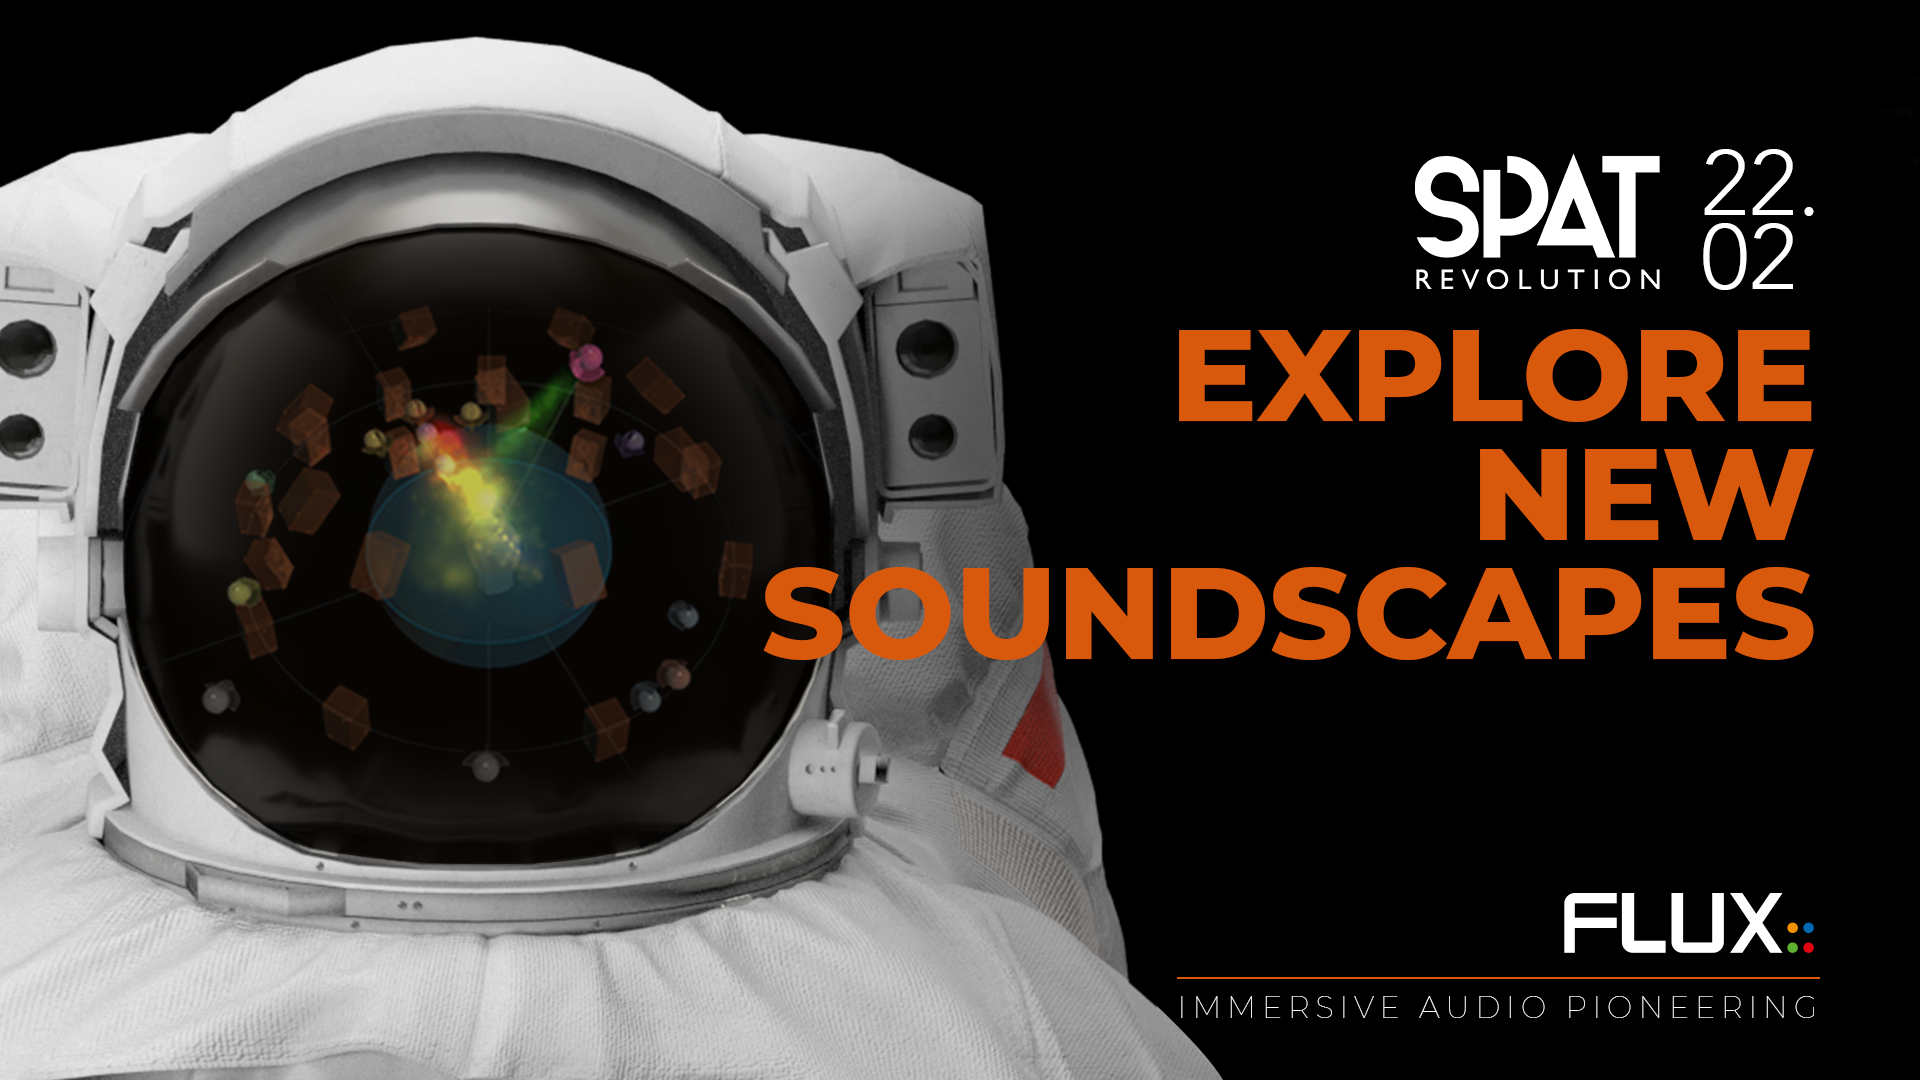
\includegraphics{index_files/mediabag/SPATionautsImage.png}

\hypertarget{a-user-guide}{%
\section{A User Guide}\label{a-user-guide}}

\textbf{Written by Cristian Vogel, Jean-Loup Pecquais, Hugo Larin and
Nicolas Erard}

with contributions from: Gäel Martinet, Vincent Carlier, Florie-Anne
Lafaye, Thibaut Carpentier, Anders Tveit and the IRCAM team.

\begin{center}\rule{0.5\linewidth}{0.5pt}\end{center}

\textbf{Legal Information}

Third edition of FLUX:: \emph{SPAT Revolution} User Guide published in
September 2022

All writing is protected under copyright © 2023 Cristian Vogel / FLUX
SOFTWARE ENGINEERING

\begin{center}\rule{0.5\linewidth}{0.5pt}\end{center}

FLUX:: is a trademark of FLUX SOFTWARE ENGINEERING All trademarks and
the logos are copyright protected.

\begin{verbatim}
FLUX:: SPAT Revolution is published by
FLUX SOFTWARE ENGINEERING
31, rue des Marais
45130 Meung-sur-Loire
R.C.S 431 616 770 ORLEANS
\end{verbatim}

IRCAMTOOLS SPAT Copyright 2023 FLUX SOFTWARE ENGINEERING and IRCAM. All
rights reserved.\\
SPAT Revolution Copyright 2023 FLUX SOFTWARE ENGINEERING and IRCAM. All
rights reserved.

\bookmarksetup{startatroot}

\hypertarget{spat-revolution---credits}{%
\chapter{SPAT Revolution - Credits}\label{spat-revolution---credits}}

\hypertarget{version-22.09}{%
\section{Version 22.09}\label{version-22.09}}

\hypertarget{user-guide-and-documentation}{%
\section{User Guide and
Documentation}\label{user-guide-and-documentation}}

\textbf{Cristian Vogel, Hugo Larin, Jean-Loup Pecquais and Nicolas
Erard}

\textbf{Additional contributions:} Gaël Martinet, Vincent Carlier,
Florie-Anne Lafaye, Thibaut Carpentier, Anders Tveit and the IRCAM team.

\hypertarget{project-manager-and-designer}{%
\subsection{Project Manager and
Designer:}\label{project-manager-and-designer}}

Gaël Martinet, Hugo Larin

\hypertarget{application-development}{%
\subsection{Application Development:}\label{application-development}}

Gaël Martinet, Florie-Anne Lafaye, Alexis Gentil, Nicolas Erard,
Siegfried Hand and Antoine Lorence.

\hypertarget{flux-dsp-design-and-development}{%
\subsection{FLUX:: DSP Design and
Development:}\label{flux-dsp-design-and-development}}

Gaël Martinet, Maxence Grandidier and Lorcan Mc Donagh

\hypertarget{spat-design-of-digital-signal-processing-algorithms-and-implementation-in-max}{%
\subsection{\texorpdfstring{``Spat\textasciitilde{}'' Design of digital
signal processing algorithms and implementation in
Max:}{``Spat\textasciitilde'' Design of digital signal processing algorithms and implementation in Max:}}\label{spat-design-of-digital-signal-processing-algorithms-and-implementation-in-max}}

Jean-Marc Jot (Espaces Nouveaux / Ircam).

\hypertarget{spat-objective-and-perceptual-characterization-of-room-acoustical-quality}{%
\subsection{\texorpdfstring{``Spat\textasciitilde{}'' Objective and
perceptual characterization of room acoustical
quality:}{``Spat\textasciitilde'' Objective and perceptual characterization of room acoustical quality:}}\label{spat-objective-and-perceptual-characterization-of-room-acoustical-quality}}

Jean-Pascal Jullien, Olivier Warusfel and Eckhard Kahle

\textbf{Additional contributions:}

Gerard Assayag, Georges Bloch, Martine Marin, Véronique Larcher,
Guillaume Vandernoot, Khoa-Van Nguyen and Markus Noisternig

\hypertarget{spat-c-dsp-code}{%
\subsection{\texorpdfstring{``Spat\textasciitilde{}'' C++ dsp
code:}{``Spat\textasciitilde'' C++ dsp code:}}\label{spat-c-dsp-code}}

Thibaut Carpentier and Remy Muller

\hypertarget{graphic-design}{%
\subsection{Graphic design:}\label{graphic-design}}

Nicolas Philippot

\hypertarget{flux-framework-development}{%
\subsection{FLUX:: Framework
development:}\label{flux-framework-development}}

Gaël Martinet, Florie-Anne Lafaye, Alexis Gentil, Bastien Prevosto,
Siegfried Hand and Antoine Lorence

\textbf{Additional contributions:} Hugo Larin, Vincent Carlier,
Jean-Loup Pecquais, Nicolas Erard, Jean Cruypenynck, Pablo Arias, Samuel
Tracol, HAL

\hypertarget{flux-framework-graphic-engine}{%
\subsection{FLUX:: Framework graphic
engine:}\label{flux-framework-graphic-engine}}

Emmanuel Julien (GS lib) and Gaël Martinet

\hypertarget{translation}{%
\subsection{Translation}\label{translation}}

\begin{itemize}
\tightlist
\item
  French: Jean-Loup Pecquais, Nicolas Erard
\item
  German: Nils Hahmann
\item
  Korean: Gong Eunju, Kim Joohna
\item
  Italian: Gianni Tamanini
\item
  Spanish: Ralph Killhertz
\end{itemize}

\hypertarget{additional-libs}{%
\subsection{Additional libs:}\label{additional-libs}}

\begin{itemize}
\tightlist
\item
  NuXPixels (Magnus Lidström)
\item
  spline lib (Joachim Klahr)
\item
  LibJpeg
\item
  Freetype 2
\item
  Zlib
\item
  Boost
\item
  RTTrPM (Blacktraxx)
\end{itemize}

\hypertarget{additional-python-modules}{%
\subsection{Additional Python
modules:}\label{additional-python-modules}}

\begin{itemize}
\tightlist
\item
  argh (Andrey Mikhaylenko)
\item
  Crypto (Dwayne C. Litzenberger)
\item
  Docopt (Vladimir Keleshev)
\item
  ecdsa (Peter Pearson)
\item
  enum (Ben Finney)
\item
  ipgetter (Fernando Giannasi)
\item
  paramiko (Jeff Forcier)
\item
  pathtools (Yesudeep Mangalapilly)
\item
  psutil (Giampaolo Rodola)
\item
  watchdog (Yesudeep Mangalapilly, Google, Inc)
\item
  yaml (Kirill Simonov)
\item
  winshell (Tim Golden)
\item
  six (Benjamin Peterson)
\item
  Request (Kenneth Reitz)
\item
  pylightxl (pydpiper)
\item
  sentry\_sdk (Copyright (c) 2018 Sentry)
\item
  urllib3 (Andrey Petrov)
\item
  certifi (Kenneth Reitz)
\item
  anytree (c0fec0de)
\item
  boltons (Copyright (c) 2013, Mahmoud Hashemi)
\item
  pendulum (Sébastien Eustace)
\item
  pytzdata (Sébastien Eustace)
\item
  msgpack (Inada Naoki)
\item
  dateutil (Gustavo Niemeyer, Paul Ganssle)
\item
  tgcrypto (Copyright (C) 2017-2020 Dan
  \url{https://github.com/delivrance})
\item
  sourcedefender (Copyright (c) 2018-2020 SOURCEdefender. All rights
  reserved.)
\end{itemize}

\hypertarget{and}{%
\subsection{And}\label{and}}

thanks to all fantastic testers\ldots{}

\hypertarget{flux-special-thanks-to}{%
\subsection{FLUX:: Special Thanks to:}\label{flux-special-thanks-to}}

Alain, Yves, Bruno and Claude for helping to shape our minds over the
years.

HAL for its support

\hypertarget{ircam-special-thanks-to}{%
\subsection{Ircam Special Thanks to}\label{ircam-special-thanks-to}}

Xavier Chabot, Eric Daubresse, Gerhard Eckel, Serge Lemouton, Gilbert
Nouno, Laurent Pottier, Manuel Poletti, Leslie Stuck, and Zack Settel
for instructive discussions and advice.

\hypertarget{ircam-rd-director}{%
\subsection{Ircam R\&D Director :}\label{ircam-rd-director}}

Hugues Vinet

\hypertarget{ircamtools-collection-manager-for-ircam}{%
\subsection{IRCAMTOOLS Collection Manager for
IRCAM:}\label{ircamtools-collection-manager-for-ircam}}

Frédérick Rousseau

\hypertarget{collection-manager-for-flux-se}{%
\subsection{Collection Manager for FLUX::
SE}\label{collection-manager-for-flux-se}}

Gaël Martinet

\hypertarget{published-by-flux-se}{%
\subsection{Published by FLUX:: SE}\label{published-by-flux-se}}

\begin{verbatim}
FLUX SOFTWARE ENGINEERING
Orléans, France,
http://www.flux.audio
Copyright 2020 FLUX SOFTWARE ENGINEERING,
All Rights Reserved.
\end{verbatim}

\texttt{IRCAMTOOLS\ SPAT\ and\ "SPAT\ Revolution"\ Copyright\ 2020\ FLUX\ SOFTWARE\ ENGINEERING\ and\ IRCAM.\ All\ rights\ reserved.}

\texttt{Spatialisateur\ and\ Spat\textasciitilde{}\ are\ trademarks\ of\ Ircam\ and\ Espaces\ Nouveaux:}

\begin{verbatim}
The Ambisonic Logo, a trademark formerly owned by Wyastone Estade Ltd, which expired
in 2010 is featured on page 30 of this guide
\end{verbatim}

\bookmarksetup{startatroot}

\hypertarget{users-and-applications}{%
\chapter{Users and Applications}\label{users-and-applications}}

\emph{SPAT Revolution} is aimed at all practitioners working in the
medium of spatial audio and 3D sound production - old and new. It is an
expert system intended for professional use but its intuitive graphical
interface invites a more diverse range of creators to engage in spatial
sound production - if it is your first experience working with spatial
sound technology, \emph{SPAT Revolution} is a great way to start out
directly at a professional quality level.

\emph{SPAT Revolution} spatialises and renders audio in real-time. It is
used in:

\begin{itemize}
\tightlist
\item
  post-production for film
\item
  studio composition
\item
  concert diffusion
\item
  virtual reality
\item
  audio for video games
\item
  360 video soundtracks
\item
  3D Audio for broadcast
\item
  interactive sound art
\item
  live production mixing
\item
  scientific research and development
\item
  sound design for film, music and theatre
\item
  environmental sound
\end{itemize}

In the contexts of live production or sound installation, the composer
or sound mixer can associate sound events with a room effect or a
specific position in space. Virtual objects can be controlled on screen,
or by a sequencer, a score-following system, or any other algorithmic
approach. Spat can easily be linked to any remote control device (show
controllers, trajectory applications, tracking systems, tablet,
smartphone, joystick, gestural sensors, etc.) through OSC and RTTrPM
interfacing protocols. \emph{RTTrPM is supported by the \emph{SPAT
Revolution} \textbf{Ultimate} license only.}

In the contexts of studio mixing and post-production, a virtual
source/object can receive its audio from individual channels on a mixing
desk or DAW with additional controllers easily set up to allow hands on
control of the positions and characteristics of virtual sources and
associated room effect. \emph{SPAT Revolution} can re-mix a multichannel
mix from one format in a virtual room that could be rendered in a
different output format, allowing a novel approach to up- and
down-mixing.

In the context of Augmented and Virtual Reality, a spatialized auditory
component is essential in creating the sensations of presence and
immersion in interactive virtual reality applications. In such
scenarios, the B-Format and binaural 3D capabilities of Spat are
particularly well suited.

An important thing to keep in mind is the long heritage and technical
expertise behind \emph{SPAT Revolution}. There are many critical factors
to consider when multichannel audio is actually applied in the real
world. But rest assured that the algorithms behind your spatial sound
project are being implemented correctly at the stage of the authoring
and rendering environment. It is good to know that \emph{SPAT
Revolution} is built with such a high level of technical expertise in
such an intuitive package.

\begin{quote}
Whatever the scale of your spatialized audio production, \emph{SPAT
Revolution} makes it simple to craft an impressive and reliable end
result.
\end{quote}

\part{Getting started}

In the following section, we will discuss how to install \emph{SPAT
Revolution}, using the FLUX:: Center, and how to redeem and activate
your licenses.

We will also explain all the differences between the \textbf{Ultimate}
and \textbf{Essential} licenses.

Furthermore, if you are searching for a quick start guide, check this
document :
\href{https://public.3.basecamp.com/p/BoK99VxRwAJ2fFM9VGSzS3Am}{quick
start guide}.

\hypertarget{installation-and-activation}{%
\chapter{Installation and
Activation}\label{installation-and-activation}}

\hypertarget{how-to-install-spat-revolution}{%
\section{How to Install SPAT
Revolution?}\label{how-to-install-spat-revolution}}

\textbf{\emph{FOUR (4) STEPS:}}

\begin{enumerate}
\def\labelenumi{\arabic{enumi}.}
\tightlist
\item
  \href{https://shop.flux.audio/en_US/login}{Create an account} on
  \href{flux.audio}{FLUX website}
\item
  License code redeem
\item
  Software license activation
\item
  Download and installation
\end{enumerate}

\hypertarget{create-and-account}{%
\section{Create and account}\label{create-and-account}}

\includegraphics{index_files/mediabag/Create.png}

\href{https://shop.flux.audio/en_US/login}{Create an account} on the
FLUX website, clicking on the previous link.

\hypertarget{redeem-a-license-code-from-activation-code}{%
\section{Redeem a License Code from activation
code}\label{redeem-a-license-code-from-activation-code}}

FLUX:: uses the iLok license management system to deliver software
licenses to users. If you have received an activation code (such as from
a dealer purchase or
\href{https://shop.flux.audio/en_US/page/trial-request-information}{30-day
trial}), you can use the Redeem License Code window to activate your
license.

\includegraphics{index_files/mediabag/RedeemLicense.png}

Visit our
\href{https://shop.flux.audio/en_US/account/licence_code_redeem}{License
Code Activation page} for more information.

\hypertarget{ilok-user-account}{%
\section{iLok User Account}\label{ilok-user-account}}

To activate licenses:


\includegraphics{index_files/mediabag/IlokLogo.png}

\begin{itemize}
\tightlist
\item
  An iLok user account is required.
\item
  An iLok USB key is optional.
\end{itemize}

FLUX:: uses the iLok license management system to deliver software
licenses to users. If you don't have an iLok account yet, please create
a free iLok account at http://www.ilok.com and download the iLok license
manager. \emph{SPAT Revolution} \textbf{Essential} license comes with
one (1) activation where the \emph{SPAT Revolution} \textbf{Ultimate}
Bundle includes two (2) activation linked to your user account. Having
two activations gives you the possibility of a fixed license on one
particular machine and a portable license on an iLok USB key if you own
one. Other examples are for main and backup SPAT Engine running on a
live production or In-studio and on-the-road scenarios.

\begin{quote}
Cloud license is currently not supported.
\end{quote}

\hypertarget{ilok-license-manager}{%
\section{iLok License Manager}\label{ilok-license-manager}}

\emph{If you have redeemed your software license or completed your
purchase process, your license will automatically be delivered into your
iLok account}

\includegraphics{index_files/mediabag/IlokManager.jpg}

For new iLok users, the first step is to download and install the iLok
license manager available on the home page of the iLok website. When
your user account is successfully activated and the iLok license manager
is correctly installed, you can start the license manager software and
log in to your iLok user account.

\hypertarget{transferring-license}{%
\section{Transferring license}\label{transferring-license}}

\includegraphics{index_files/mediabag/iLokManagerTransfer.jpg}

Pressing on the sign-in button will allow you to connect to your
account. After Logging in, you are now ready to transfer any licenses to
a computer or to any iLok USB key if you happen to have one. The process
of transferring a license is as simple as dragging the license from the
Available tab to your Local Computer \emph{(or iLok key)} on the left
side. \emph{SPAT Revolution} \textbf{Essential} license is a single
license where \emph{SPAT Revolution} \textbf{Ultimate} is a bundle
containing three (3) licenses, \textbf{Essential}, \textbf{Ultimate} and
\textbf{Legacy}.

\textbf{Simply drag your license to your Local Computer or on an iLok
USB key. You are now set!}

\begin{quote}
If you require further information about iLok and managing licenses
please refer to iLok.com website.
\end{quote}

\hypertarget{flux-center}{%
\section{FLUX:: Center}\label{flux-center}}

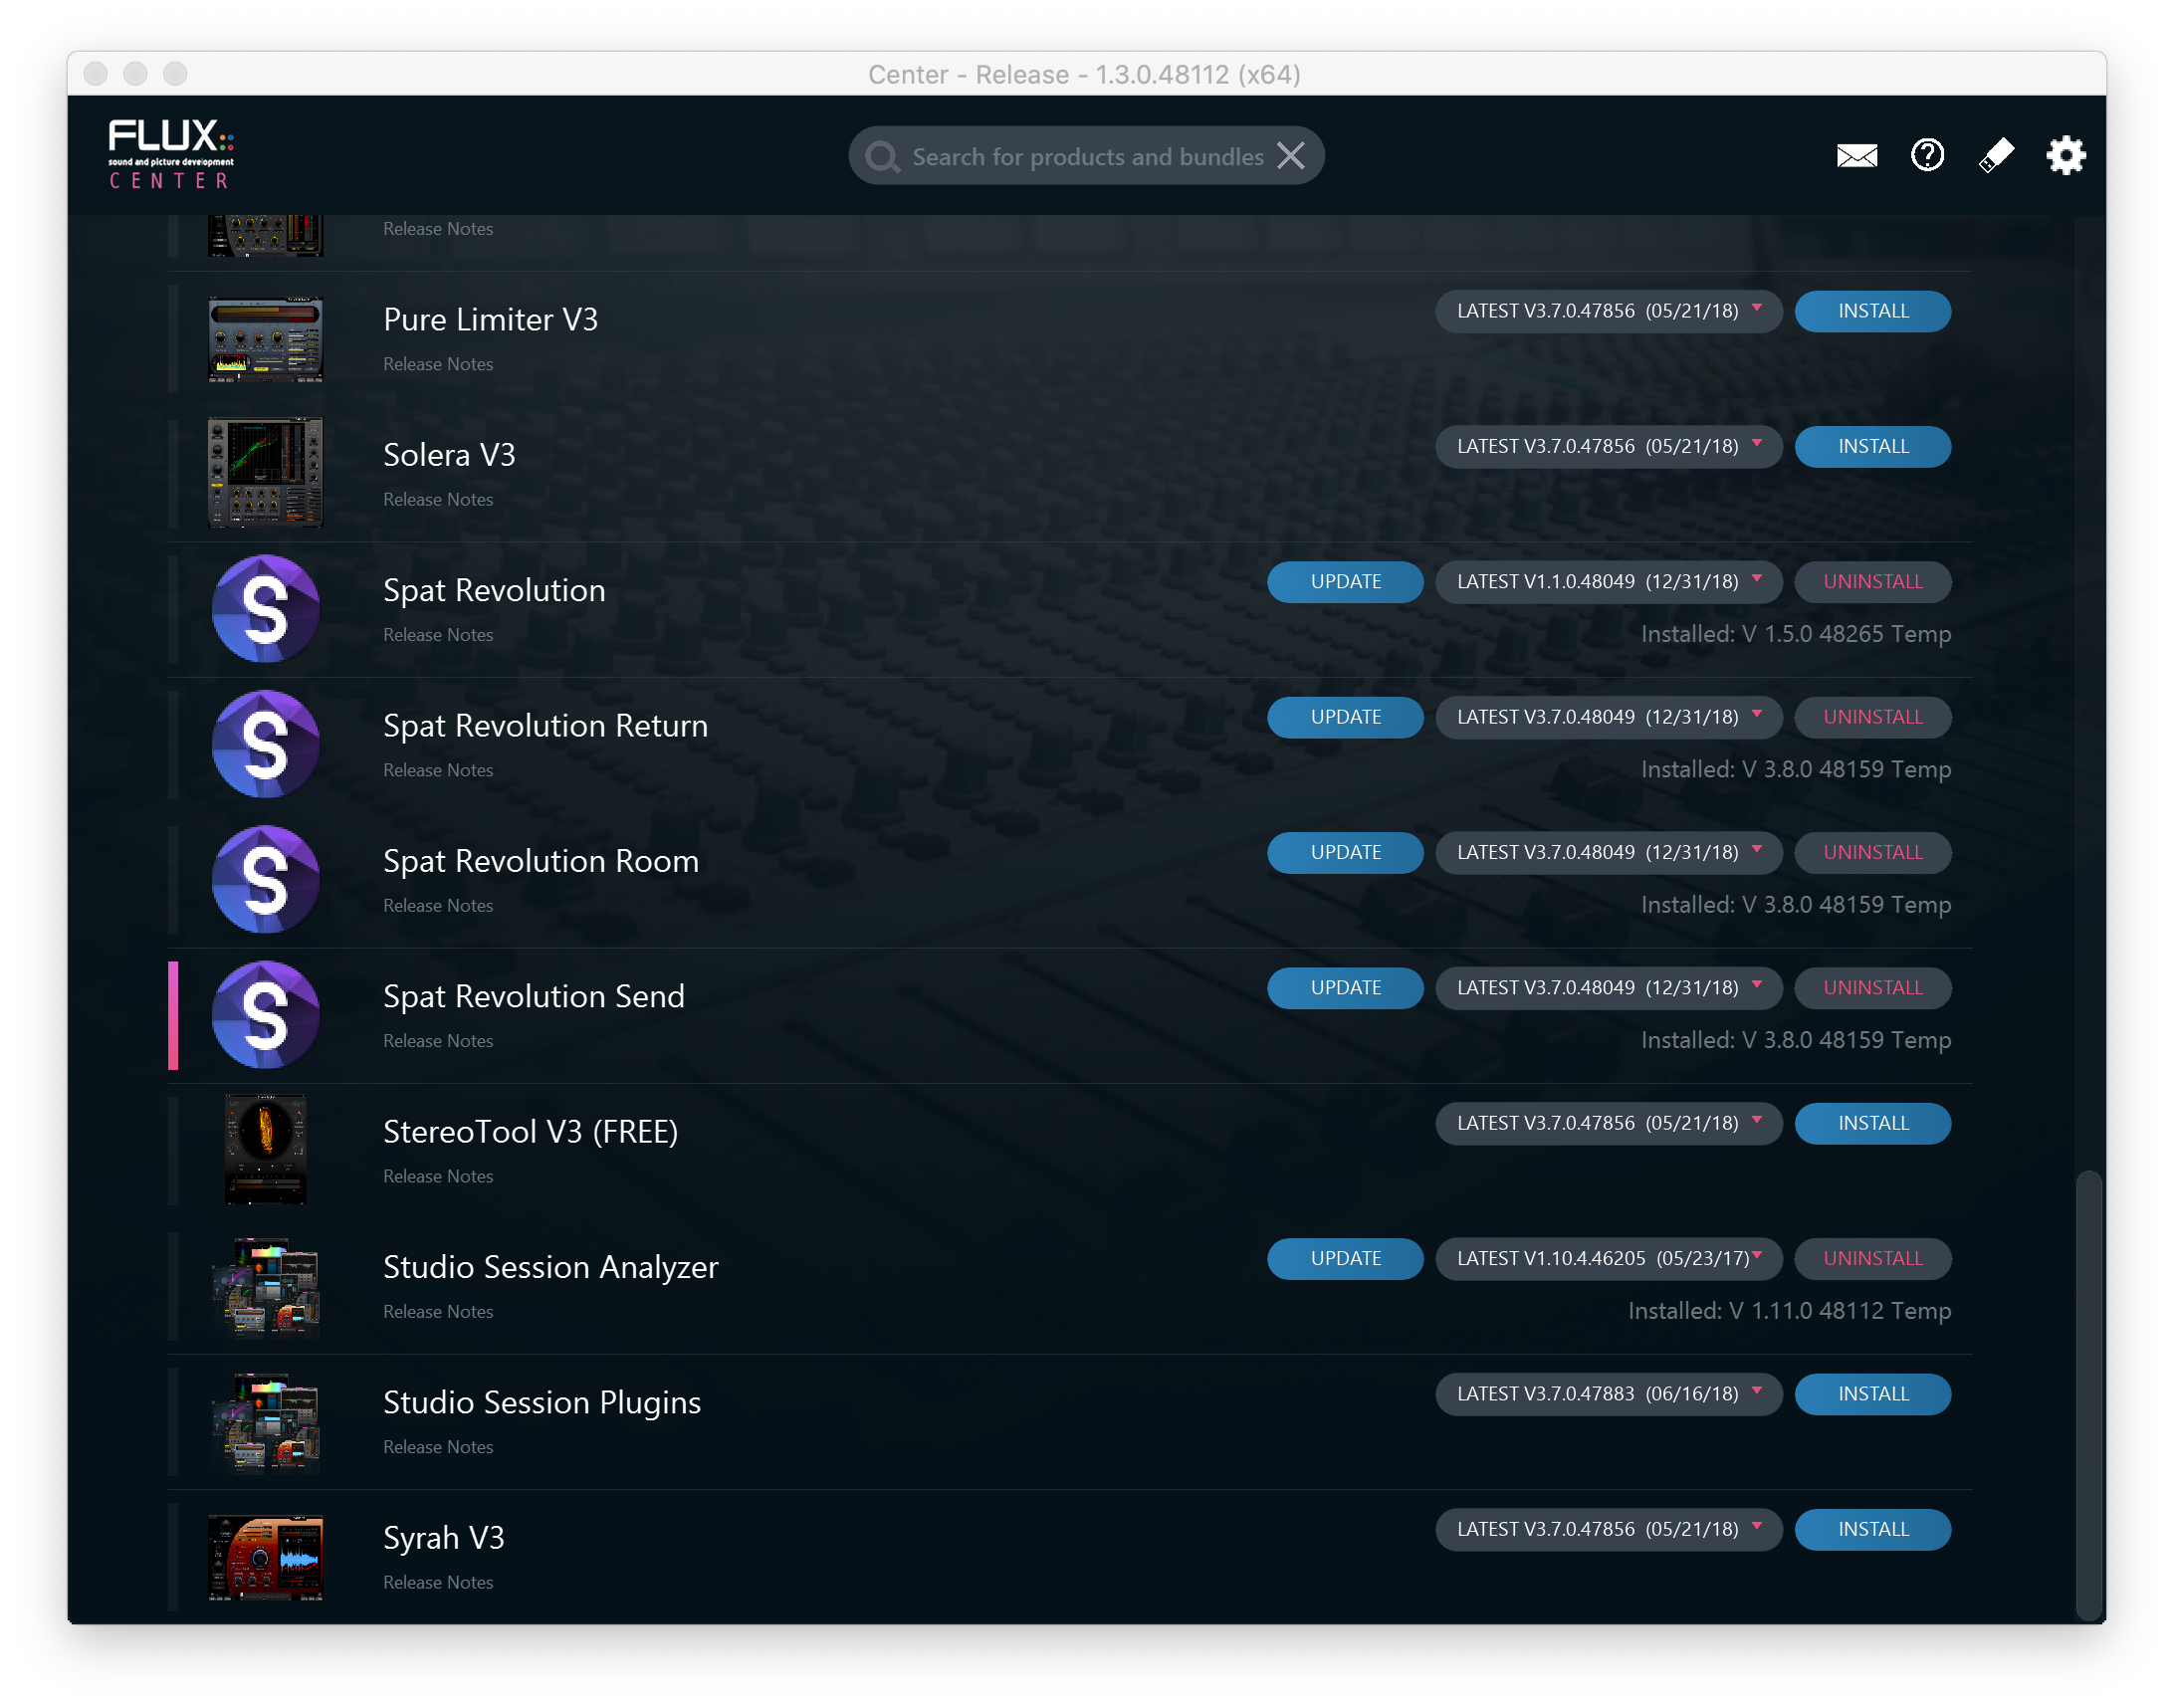
\includegraphics{index_files/mediabag/Page.png}

Next step is to get the installers for the FLUX:: products you are
licensed for. All the software and plugins from FLUX:: are available via
our FLUX:: Center software. This is a Mac or Windows application we have
created to help keep your FLUX:: products up to date and to give you a
clear overview of what you have installed. Firstly, please visit the
download section of the FLUX:: Website to get the installer for the
\href{https://flux.audio/download/}{FLUX:: Center application.}

On this page you will find a macOS, a Windows 64 bits. As well are
provided legacy version for older operating systems. After downloading
and installing, you can open the FLUX:: Center applications to begin the
process of installing the \emph{SPAT Revolution} software.

!\textgreater{} An authentication is required at the launch of FLUX::
Center. This is the login details of your FLUX shop account which allows
you to see only your products licensed for (temporary or permanent).

\hypertarget{center-preferences}{%
\section{Center Preferences}\label{center-preferences}}


\includegraphics{index_files/mediabag/TopBar.jpg}

When you open FLUX:: Center you will see a page that lists all FLUX::
products available for you to install. You will also find information
about which version you have currently installed on your system and
which new versions might be available for you to update to. You can
select versions to install - or uninstall if necessary - using the pull
down menus. If you would like to access more installer options such as
your preferred plug-in format, please click on the gear icon to the top
right of the header area.

\hypertarget{center-preferences-and-options}{%
\section{Center Preferences and
Options}\label{center-preferences-and-options}}

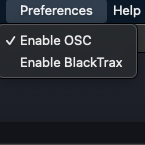
\includegraphics{index_files/mediabag/Preferences.png} \textgreater{}
\emph{\emph{SPAT Revolution} Send/Room/Return plugins are available in
VST-64bit, AU-64bit and AAX-64bit only.}

This preference page will allow you to choose various installation
options such as preferred plug-in formats for your system. Choosing your
format and returning to the main page by pressing the OK button will
show all your install options for software and plugins based on the
desired formats chosen.

If you would like to be closer to the most current development cycles of
the software, you can enable the Beta Versions option. This will give
you access to a special set of software installers from the pull down
menus on the main FLUX:: Center page. Beta versions are the new builds
that are still under development but may contain useful bug fixes and
new features. If you find that a beta version is not stable enough for
you, then you can always roll back to a stable release version at any
time through the FLUX:: Center installers. Note that these versions
starts with a B where official releases start with a V.

\hypertarget{ultimate-and-essential-licenses}{%
\chapter{Ultimate and Essential
licenses}\label{ultimate-and-essential-licenses}}

\emph{SPAT Revolution} comes in different flavors: an \textbf{Essential}
and an \textbf{Ultimate} licenses. Both share the same audio engine and
powerful 3D audio capabilities.

The \textbf{Essential} license aims to be a limited version of
\textbf{Ultimate}: same workflow but limited capacities at reduced
price.

\hypertarget{ultimate-and-essential-whats-common}{%
\section{Ultimate and Essential : what's
common?}\label{ultimate-and-essential-whats-common}}

The \emph{SPAT Revolution} software supports with the same installer
(binary) both license options and has the common features listed below:

\begin{itemize}
\tightlist
\item
  An easy-to-understand setup page, showing a clear representation of
  the signal path.
\item
  A powerful mixing environment, using a 3D view and perceptive factor
  parameters.
\item
  An oriented-object audio engine allowing the user to render either
  channel-based, Higher Order Ambisonic (HOA) or binaural audio streams.
\item
  Support for mono, stereo and multichannel inputs streams.
\item
  A flexible speaker array editor allowing going beyond the usual
  standards.
\item
  A snapshot system to easily recall scenes on the fly.
\item
  An audio pipe technologies allowing receiving and sending audio from
  all the major DAW to and from \emph{SPAT Revolution}.
\item
  An exhaustive list of OSC commands to allow a deep remote control of
  \emph{SPAT Revolution}.
\end{itemize}

\hypertarget{ultimate-and-essential-differences}{%
\section{Ultimate and Essential:
differences}\label{ultimate-and-essential-differences}}

The main limitations of the \textbf{Essential} license are:

\begin{itemize}
\tightlist
\item
  The number of cumulated input channels is limited to 32.
\item
  The number of cumulated output channels is limited to 18.
\item
  The number of rooms is limited to 1: no simultaneous rendering.
\item
  HOA order is limited to 3rd order.
\item
  Tracking data cannot be modified
\item
  RTTrp is not allowed.
\end{itemize}

\textbf{Complete specification is available
\href{https://www.flux.audio/project/spat-revolution/\#specifications}{here}.}

\hypertarget{ultimate-and-essential-sessions-compatibility}{%
\section{Ultimate and Essential sessions
compatibility}\label{ultimate-and-essential-sessions-compatibility}}

When creating or opening a session that contains elements non-compatible
with the \textbf{Essential} license, those elements are simply
deactivated (not processed). Thus, an \textbf{Ultimate} session can be
opened with an \textbf{Essential} license and vice-versa. See
\href{Spat_Environment_Modules_de_activation.md}{Modules (de)activation
and sessions compatibility}.

\hypertarget{check-essential-compatibility}{%
\subsection{Check Essential
compatibility}\label{check-essential-compatibility}}

In the top bar menu, click on File \textgreater{} Check Essential
Compatibility to check if the current session is compatible with the
SPAT Essential restrictions.

\includegraphics{index_files/mediabag/EssentialAlreadyCompatible.png}

If the session is not compatible, it can be opened with an
\textbf{Essential} license, the restrictions due to license limitations
will automatically deactivate the non-authorized objects.

\begin{quote}
If a session contains elements non-compatible with an \textbf{Essential}
license, they can be manually deactivated for the session to fit the
\textbf{Essential} license restrictions. If all the non-authorized
elements are inactive, the session is considered as compatible with
\textbf{Essential} license.
\end{quote}

See \href{Spat_Environment_Modules_de_activation.md}{Modules
(de)activation} for more information about automatic and manual
(de)activation.

\hypertarget{essential-compatibility-mode-in-ultimate}{%
\subsection{Essential compatibility mode in
Ultimate}\label{essential-compatibility-mode-in-ultimate}}

The \textbf{Ultimate} license offers an \emph{Essential Compatibility
Mode}, for switching between \textbf{Essential} and \textbf{Ultimate}
behaviors without any change in your license authorization.

\includegraphics{index_files/mediabag/EssentialCompatibilityModeOn.png}

\part{Spatialization Technology}

In this section, we will discuss on the various spatialization tool used
by \emph{SPAT Revolution}.

Here are some straight to the point key points:

\begin{itemize}
\tightlist
\item
  \emph{SPAT Revolution} is an object-based audio engine. The mixes you
  will create will consist in sets of data for each sound object. These
  data sets will then be decoded for a certain type of spatialization
  technique.
\end{itemize}

\begin{quote}
With \emph{SPAT Revolution} \textbf{Ultimate} license, several render
can be done at the same time (multi-room).
\end{quote}

\begin{itemize}
\tightlist
\item
  Thanks to the object-based engine, you can create sound stages in all
  spatialized audio format possible: channel-based, ambisonics (up to
  seventh order), binaural and transaural. If these names does not ring
  a bell to you, do not fear, we will cover these different techniques
  later in this section.
\item
  On top of the object-based engine, \emph{SPAT Revolution} also covers
  the acoustic simulation side of things. The build-in reverberation
  will adapt to your mixes, and, more importantly, to your desired
  output format.
\item
  \emph{SPAT Revolution} aims at many use cases, many of them being for
  live performances. It was designed to not add any more latency than
  necessary on the signal path.
\end{itemize}

Let's start with an important notion of spatial audio: the listener
position.

\hypertarget{listener-position}{%
\chapter{Listener Position}\label{listener-position}}

The impression of positioned audio which is rendered on a speaker array
is generally successful when a listener is situated in the optimum
position to perceive it, the so-called \emph{Sweet Spot}. Thanks to the
popularity of stereo sound, people tend to know that if you want to hear
a good stereo image, you should place yourself in front of the two
speakers and stand somewhere in the middle. That's a good way to
describe the \emph{Sweet Spot} to an audience or client.

In more complex speaker arrangements, the \emph{Sweet Spot} is usually
considered to be the area that all the speakers, or sound emitters in a
virtual space, are pointing to. It has the Cartesian coordinates of
(0,0,0) in relation to the speaker positions. In \emph{SPAT Revolution},
the optimum listening area is represented by the dummy head and the
inner circle that surrounds it.

\includegraphics{index_files/mediabag/3DViewFrontHead.png}

The dummy head indicates the \emph{Listener Position}. In \emph{SPAT
Revolution}, the \emph{Listener Position} is actually a bit more useful
than just an indication of the \emph{Sweet Spot}. In general, it is
useful for getting some bearings in the spatial composition. Knowing
which direction the \emph{Listener Position} is facing, helps you
understand the spatial image and place sources correctly. For example, a
train audibly approaches from the left in an ambisonic field recording
you are working with as a source, but it visually approaches from the
right on the video footage you are editing to. You can use the listener
position as a reference point to transform the field recording correctly
so that it correlates to what's happening on screen. Also, when working
in ``stage'' oriented spaces, the listener position in a SPAT Room will
help you compose a scene with the correct relationship to the front,
back and sides of the space. It also provides a method for giving a
sense of distance to a sound source by placing virtual sound objects
closer or farther away from the \emph{Listener Position}. The internal
distance perceptual cues, such as air absorption, doppler and gain drops
are all calculated in relation to the \emph{Listener Position}.

\begin{quote}
Some Panning and Stream Types have wider \emph{Sweet Spots} than others
and some do not have a \emph{Sweet Spot} at all.
\end{quote}

It is worth noting that there are some panning algorithms in \emph{SPAT
Revolution} that are \textbf{not} \emph{Sweet Spot} dependent. These are
more suitable for use on arbitrarily positioned speaker distributions.
We will get to them shortly.

!\textgreater{} The dummy head is only visible for \emph{Sweet Spot}
dependent panning types.

\begin{quote}
The Listener Position can be moved in a \emph{SPAT Revolution} room.
\end{quote}

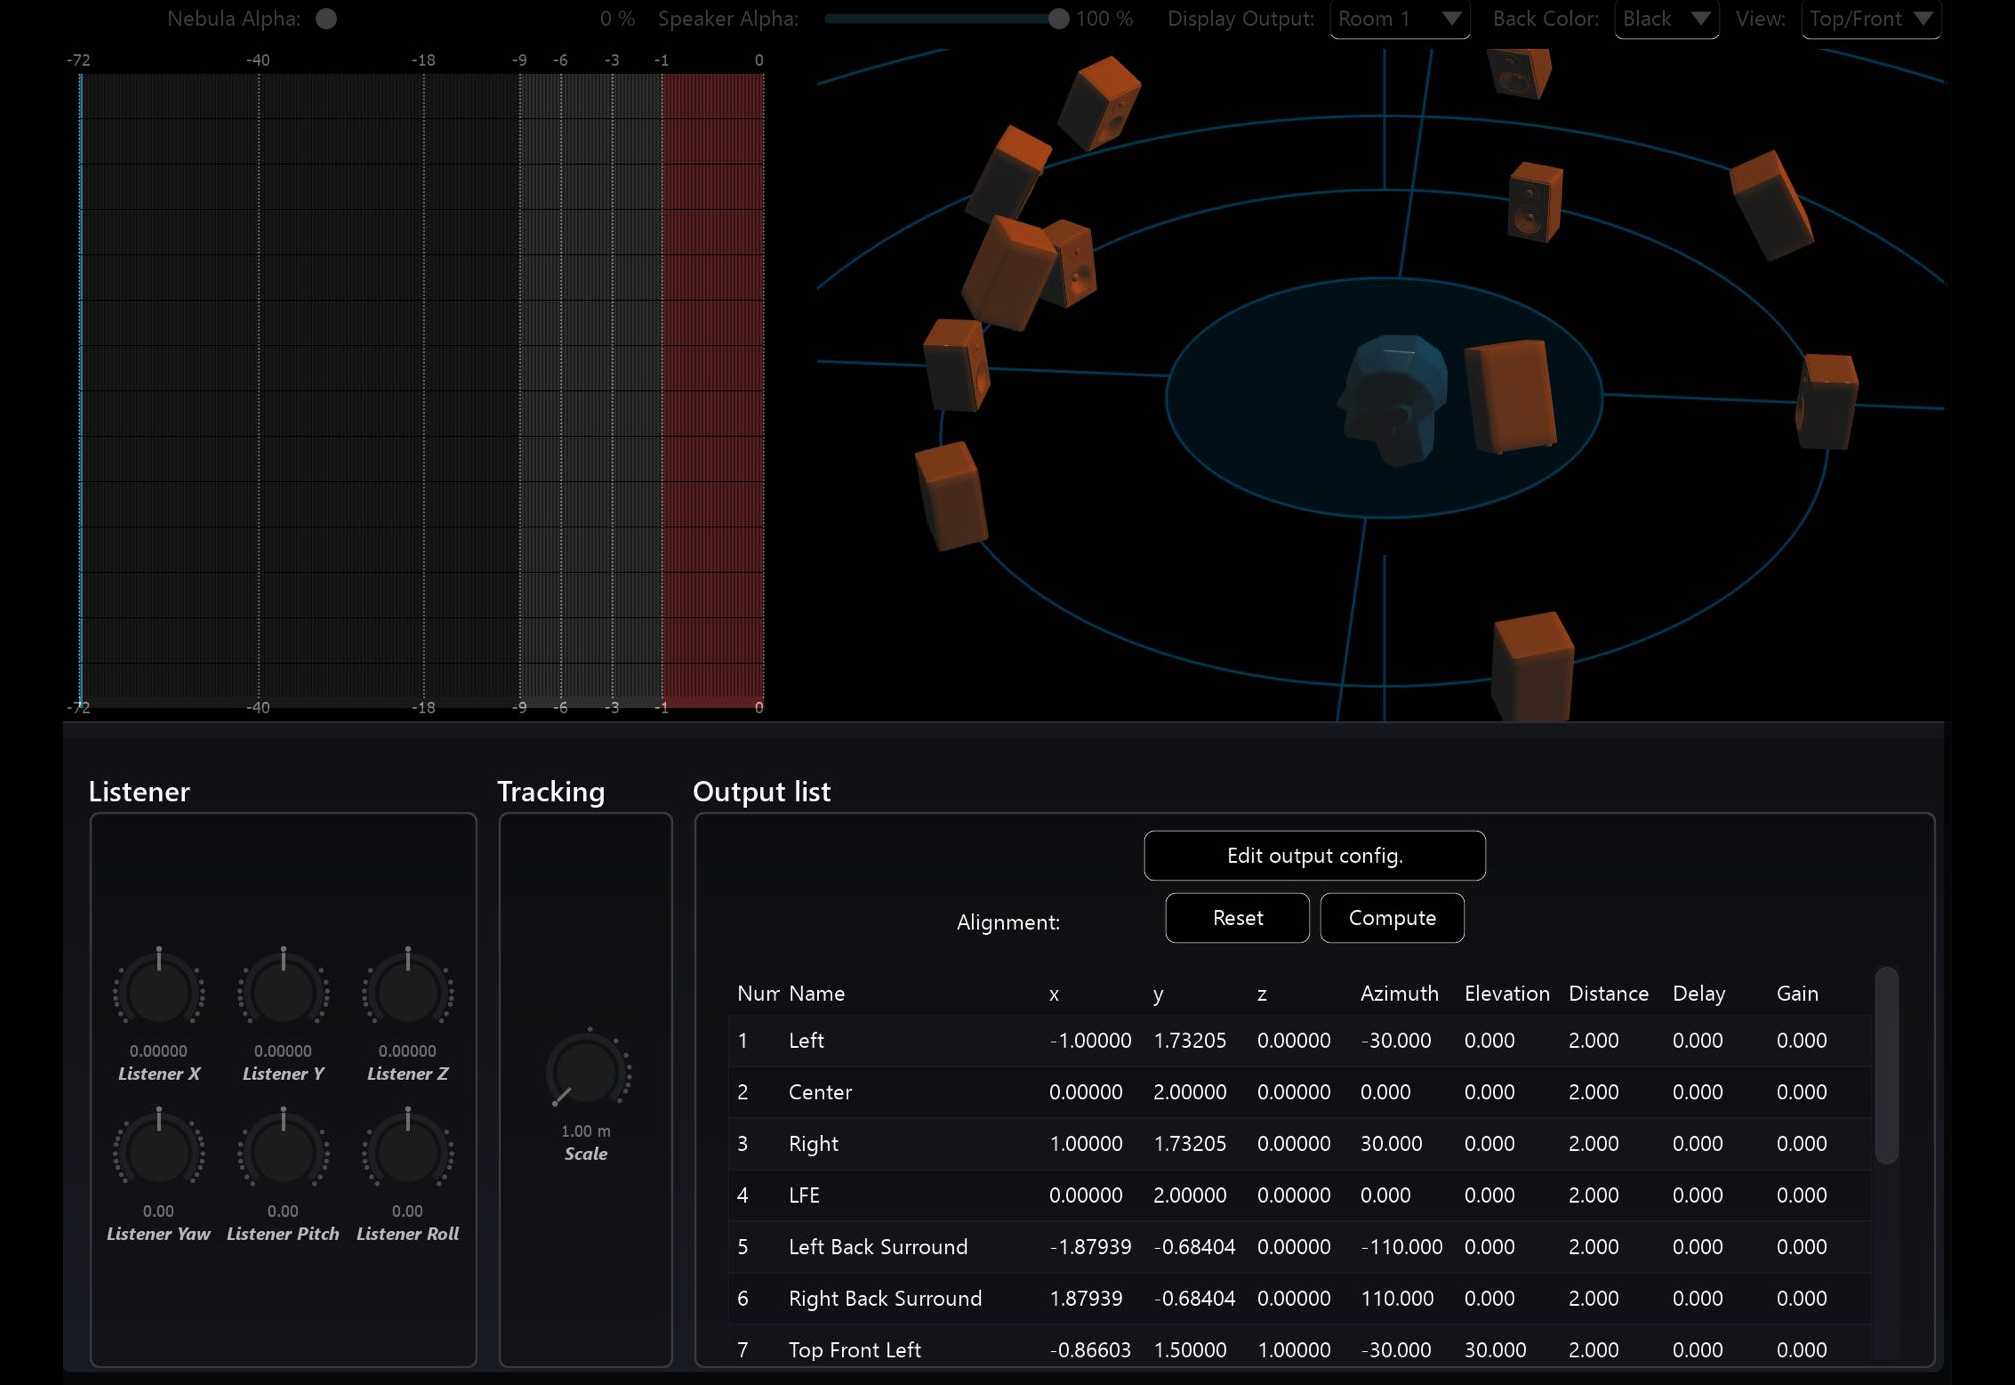
\includegraphics{index_files/mediabag/OutputChannelBased.png}

\hypertarget{listener-position-and-head-tracking}{%
\section{Listener position and head
tracking}\label{listener-position-and-head-tracking}}

In certain advanced situations which might combine position tracking
systems with real time binaural audio, it is even possible to transform
the \emph{Listener Position} in \emph{SPAT Revolution}. One application
of this might be to give the sensation of getting closer to a sound
emitter inside a virtual scene for a headset wearing participant at an
interactive VR installation. Given the camera position perspective to
the listener is as well possible by mapping camera position to the
\emph{Listener Position} of SPAT Revolution.

\hypertarget{binaural}{%
\chapter{Binaural}\label{binaural}}

\hypertarget{introduction}{%
\section{Introduction}\label{introduction}}

The word ``binaural'' covers various methods of sound recordings,
synthesis and reproduction which can render 3D spatial audio content
over headphones. For instance, binaural field recordings can be made by
placing miniature microphones in the ear canals of a listener or of a
dummy head (like ' \textbf{Kemar} ' or ' \textbf{KU100} ') and when
played back over headphones such recordings can produce an authentic
immersive auditory experience with enhanced spatial aspects. Relatively
recent progress in signal processing technology has made it possible to
synthesize binaural signals without the need of microphones.

Using binaural synthesis, a sound can be arbitrarily positioned around a
listener synthesizing the sensory experience of an extended
spatialization. Like some other two-channel formats such as Mid-Side
Stereo, binaural-encoded audio recordings are not compatible with stereo
speakers. If a binaural encoded audio file is played on a normal stereo
setup, audio will be heard, but it won't sound good.

!\textgreater{} It is important to point out to a client who might be
new to binaural monitoring, \emph{that binaural files should only be
listened to on a good pair of headphones.}

\hypertarget{hrtf}{%
\section{HRTF}\label{hrtf}}

HRTF is an abbreviation for \emph{Head Related Transfer Function}. This
function is a mathematical model of the filtering effect caused by a
listener's own head, external ear and torso. This filtering plays a
significant role in the way we localize sounds around us and is unique
to every individual. HRTF is different between the two ears, so we
always talk about pairs of HRTFs.

When synthesizing binaural monitoring, a perfect result could be
attained by rendering through the exact HRTFs that matches the body
filtering effect of an individual. In practice this is not easily done,
so \emph{SPAT Revolution} offers many choices of pre-analyzed HRTFs
profiles which you can apply for monitoring and encoding binaural audio.
You can manage the selection of HRTFs profiles in the \emph{SPAT
Revolution} Preferences where you will find a number of different
profiles including the option to load your own HRTFs. The default HRTFs
is the Kemar dummy head model, which is often used as an all-round
generic head and shoulder filter.

\hypertarget{hrtf-profiles}{%
\section{HRTF Profiles}\label{hrtf-profiles}}

The included HRTFs profiles in \emph{SPAT Revolution} are taken from a
number of large-scale laboratory research projects where measurements
were taken on many individuals*. The chances are that one person's ears
may sound more natural to you than others. For a quick way to monitor
binaural, you should try to find a profile that you feel most
comfortable with when monitoring your virtual scene on headphones. If
you are providing a 3D in-ear monitor mix for a performer or a visitor
to an installation, try to find an HRTFs profile that suits them best.
This can be fun! If you are not comfortable listening through someone
else ears ---which is understandable--- you could look into creating a
personalized HRTFs profile from your own head and upper torso
measurements. There already exist a number of services that can create
HRTFs profiles taken from laboratory measurements. If you decide to do
this, for yourself or someone else, then you can add the personalized
profile to the list in the HRTFs Manager. In fact, you can import any
HRTFs in SOFA format to the \emph{SPAT Revolution} binaural encoding
list, making \emph{SPAT Revolution} a very flexible solution for
binaural monitoring and rendering.

!\textgreater{} \emph{An imported HRTFs profile should be in SOFA format
and should match the sample rate of your project. It is preferable to
use a ``SimpleFreeFieldSOS'' IIR type of HRTFs.}

* The profiles come from the ``LISTEN'', ``CROSSMOD'' and ``BiLi''
databases.

\hypertarget{binaural-algorithms}{%
\section{Binaural algorithms}\label{binaural-algorithms}}

\hypertarget{standard-binaural-mode}{%
\subsection{Standard binaural mode}\label{standard-binaural-mode}}

This mode uses the selected HRTFs profile in order to recreate the sound
field.

\hypertarget{advanced-algorithms}{%
\subsection{Advanced algorithms}\label{advanced-algorithms}}

\hypertarget{near-field-binaural}{%
\subsubsection{Near-field binaural}\label{near-field-binaural}}

HRTFs are generally measured at one or two meters of the listener. In
reality, the HRTFs are changing with the distance between the source and
the listener, especially when sources are close.

The Near Field Binaural tends to recreate close HRTFs, with an
additional filter set applied.

\hypertarget{spherical-head-model}{%
\subsubsection{Spherical head model}\label{spherical-head-model}}

This binaural synthesis simulates the head like a rigid sphere, instead
of using HRTFs.

As this model does not use HRTFs, this synthesis consumes less CPU.
However, the localization is clearly less precise.

\hypertarget{snowman-model}{%
\subsubsection{Snowman model}\label{snowman-model}}

This synthesis is the improvement of the Spherical Head Model. Besides
the head reflections, torso ones are simulated, like two spheres one on
the top of the other. Hence, its name, ``snowman model.''

\hypertarget{head-scale-parameter}{%
\subsection{Head scale parameter}\label{head-scale-parameter}}

The parameter ``head scale'', available for the four binaural
algorithms, allows adapting the head size to the listener. This will
adjust the interaural time and level differences. It is available on the
room parameter on the \textbf{Setup} page, but also on the output panel
of the room.

\begin{figure}

{\centering \includegraphics{index_files/mediabag/HeadScaleParameter.png}

}

\caption{Headscale parameter}

\end{figure}

\hypertarget{binaural-monitoring-module}{%
\section{Binaural Monitoring Module}\label{binaural-monitoring-module}}

\begin{figure}

{\centering 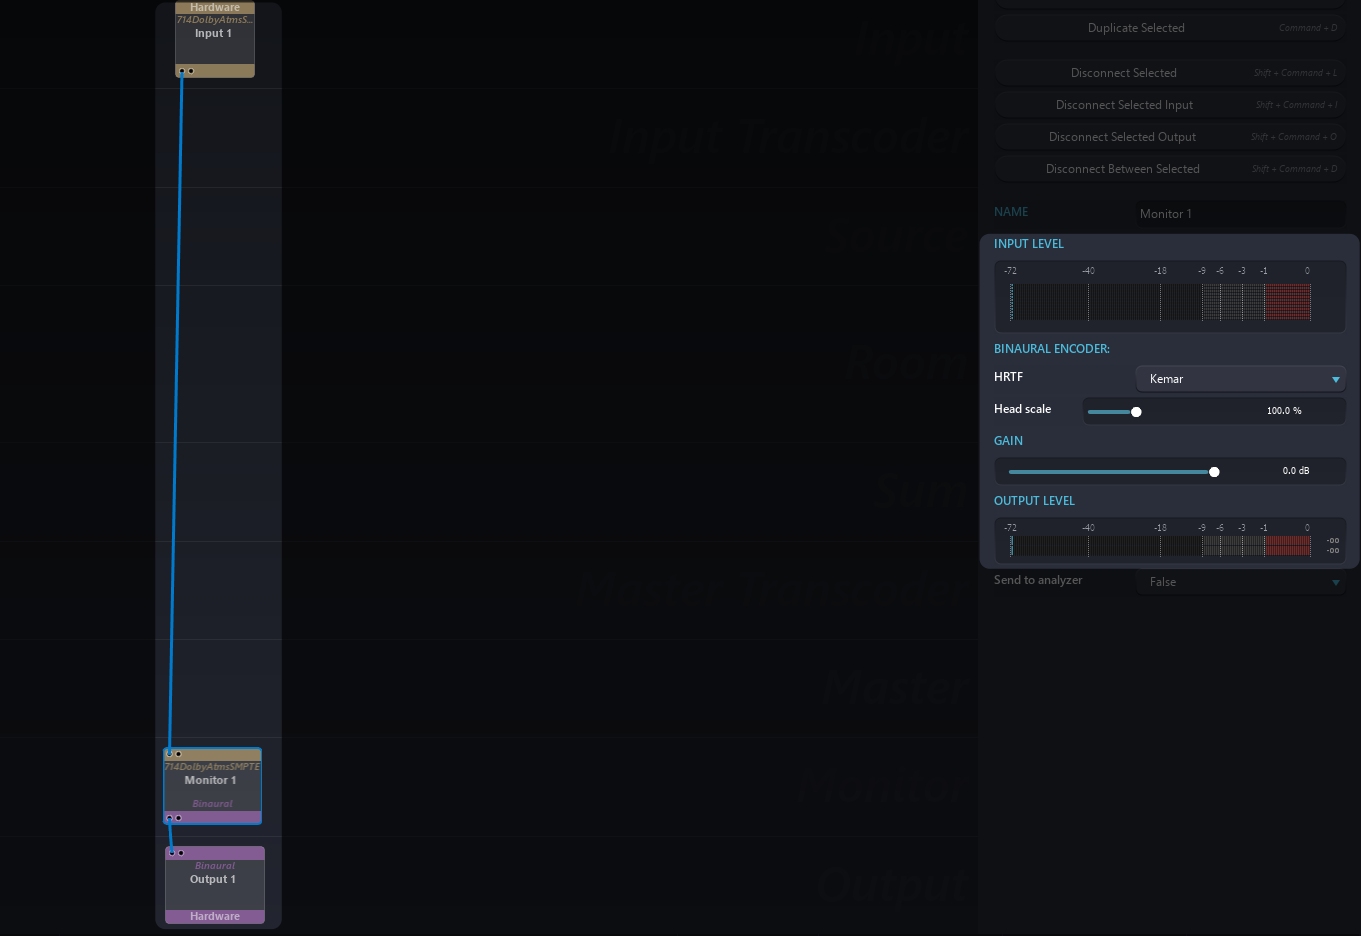
\includegraphics{index_files/mediabag/BinauralMonitor.png}

}

\caption{Binaural Monitor}

\end{figure}

In the \emph{Setup} page of \emph{SPAT Revolution}, you will find a
module dedicated to binaural monitoring. Its purpose is to monitor any
kind of speaker setup using headphones and binaural encoding. This can
give you an impression of how your spatialization might sound on a
particular channel based system when you are off location.

You can add a \textbf{binaural monitoring module} by clicking on the +
icon of the Monitor row towards the bottom of the \emph{Setup} page
graph. The module is very simple to use. It will automatically detect
the type of channel based audio stream you connect into it.

The binaural monitoring module works by virtualizing each speaker, not
each source, so any real world speaker phenomena will be reflected in
the binaural rendering. For example, a virtual source positioned in the
center between two virtual speakers will be rendered with the same
``phantom speaker'' in the binaural monitoring as in the physical world,
because there is no virtual speaker at the center point either.

To listen to the binaural stream on headphones, you should select the
HRTFs profile you would like to use for the encoding, and connect the
output from the module to a dedicated Output module at the bottom of the
graph. The output should be routed to the headphone monitor outputs of
your audio hardware.

\hypertarget{transaural}{%
\chapter{Transaural}\label{transaural}}

Although we said earlier that binaurally encoded files are not
compatible with stereo loudspeaker systems, it turns out that in
\emph{SPAT Revolution} there is a way to play binaurally encoded signals
on loudspeakers if necessary. You can do this by transcoding a binaural
stream into a Transaural stream either at the \emph{Input Transcoder}
stage or at the \emph{Master Transcoder} stage of the \textbf{Setup}
page graph.

The term \emph{Transaural} refers only to the transcoding of binaural
signals into loudspeaker-compatible signals. The reproduction mode is
also known as ``cross-talk cancellation'' as it uses this very process
to establish the loudspeaker-compatible signals.

!\textgreater{} To successfully achieve cross-talk cancellation, it is
assumed that the listener \emph{will be placed at a particular position
with respect to the loudspeaker pair}, or the spatial information will
not be properly perceived. The loudspeaker pair need to be positioned as
a regular stereo setup, Left at -30 degrees and Right at +30 degrees.

An optimum listening position such as that needed for Transaural
decoding, is also known as the \emph{Sweet Spot} (see
\href{Spatialisation_Technology_Listener_Position.md}{\emph{Listener
Position}}). It is a fundamental concept to be aware of as we move into
the next section: \emph{Channel Based} streams and panning algorithms.

\hypertarget{channel-based-streams}{%
\chapter{Channel Based Streams}\label{channel-based-streams}}

We have already covered the two-channels binaural stream type for
monitoring and final encoding into a binaural format. One of the other
important Stream Types is referred to as \emph{Channel Based}. This
stream can range from a single-channel mono to a multichannel audio
stream (*). These streams will flow as a perfectly synchronized group
through the signal graph defined in the \emph{Setup} page. The channel
count of the stream is set by the choice in the \emph{Speaker
Arrangement} pull down menu of a module. A change to the speaker
configuration here alters the channel count in and out of a module,
depending on its context in the signal graph. When you connect
channel-based modules together in \emph{SPAT Revolution}, they
automatically inherit the speaker arrangement and channel count from the
stream type at their connected input.

!\textgreater{} * The \textbf{Essential} license limits the total number
channels to 32 input channels and to 18 outputs channels.

Channel based audio streams - when connected to a hardware output module
- will render the spatial composition on speakers connected to the
physical outputs of your audio hardware. \emph{SPAT Revolution} is
expecting the loudspeaker system specified in the speaker arrangement of
the \emph{Output} module. If the real loudspeaker arrangement does not
correctly match the speaker arrangement model or there is a mistake in
your routing somewhere, the spatial sound image will then be
compromised.

!\textgreater{} Each output channel must be routed to the correct
speaker.

The golden rule for spatialization using channel-based audio is that
each rendered channel must be connected only to its corresponding sound
emitter in the destination system. An exact correlation from the model
to the physical system is assumed by the calculations inside each of the
panning algorithms. If the installation is not right for some reason, a
listener may experience something with spatial aspects, but not with the
intended quality. To correctly install and tune a multichannel sound
system is one of the more challenging aspects of working with spatial
composition and performance systems. So many things can compromise the
spatial image, and sometimes it is hard to tell by ears.

In order to try and simplify this process in practice, certain labeling
conventions are used by engineers and designers to identify which
speaker belongs to which channel. When channel counts are high, angular
positioning and distance measurements are used to identify the correct
speaker routing. In \emph{SPAT Revolution's} \textbf{Speaker Arrangement
editor}, you additionally get a 3D graphical rendering of the sound
system, where you can select speakers which will be visually identified,
so you can label them clearly. These labels will be saved into a speaker
arrangement profile, so you can get some more consistent reference
points when routing.

\begin{longtable}[]{@{}lll@{}}
\toprule()
Left & Centre & Right \\
\midrule()
\endhead
Left Surround & LFE & Right Surround \\
Left Back Surround & Center Back Surround & Right Back Surround \\
Top Back Left & Top Front Center & Top Back Right \\
Left Surround Rear & VOG & Right Surround Rear \\
Top Front Left & Back Center & Top Front Left \\
\bottomrule()
\end{longtable}

\begin{quote}
Some common speaker channel naming conventions.
\end{quote}

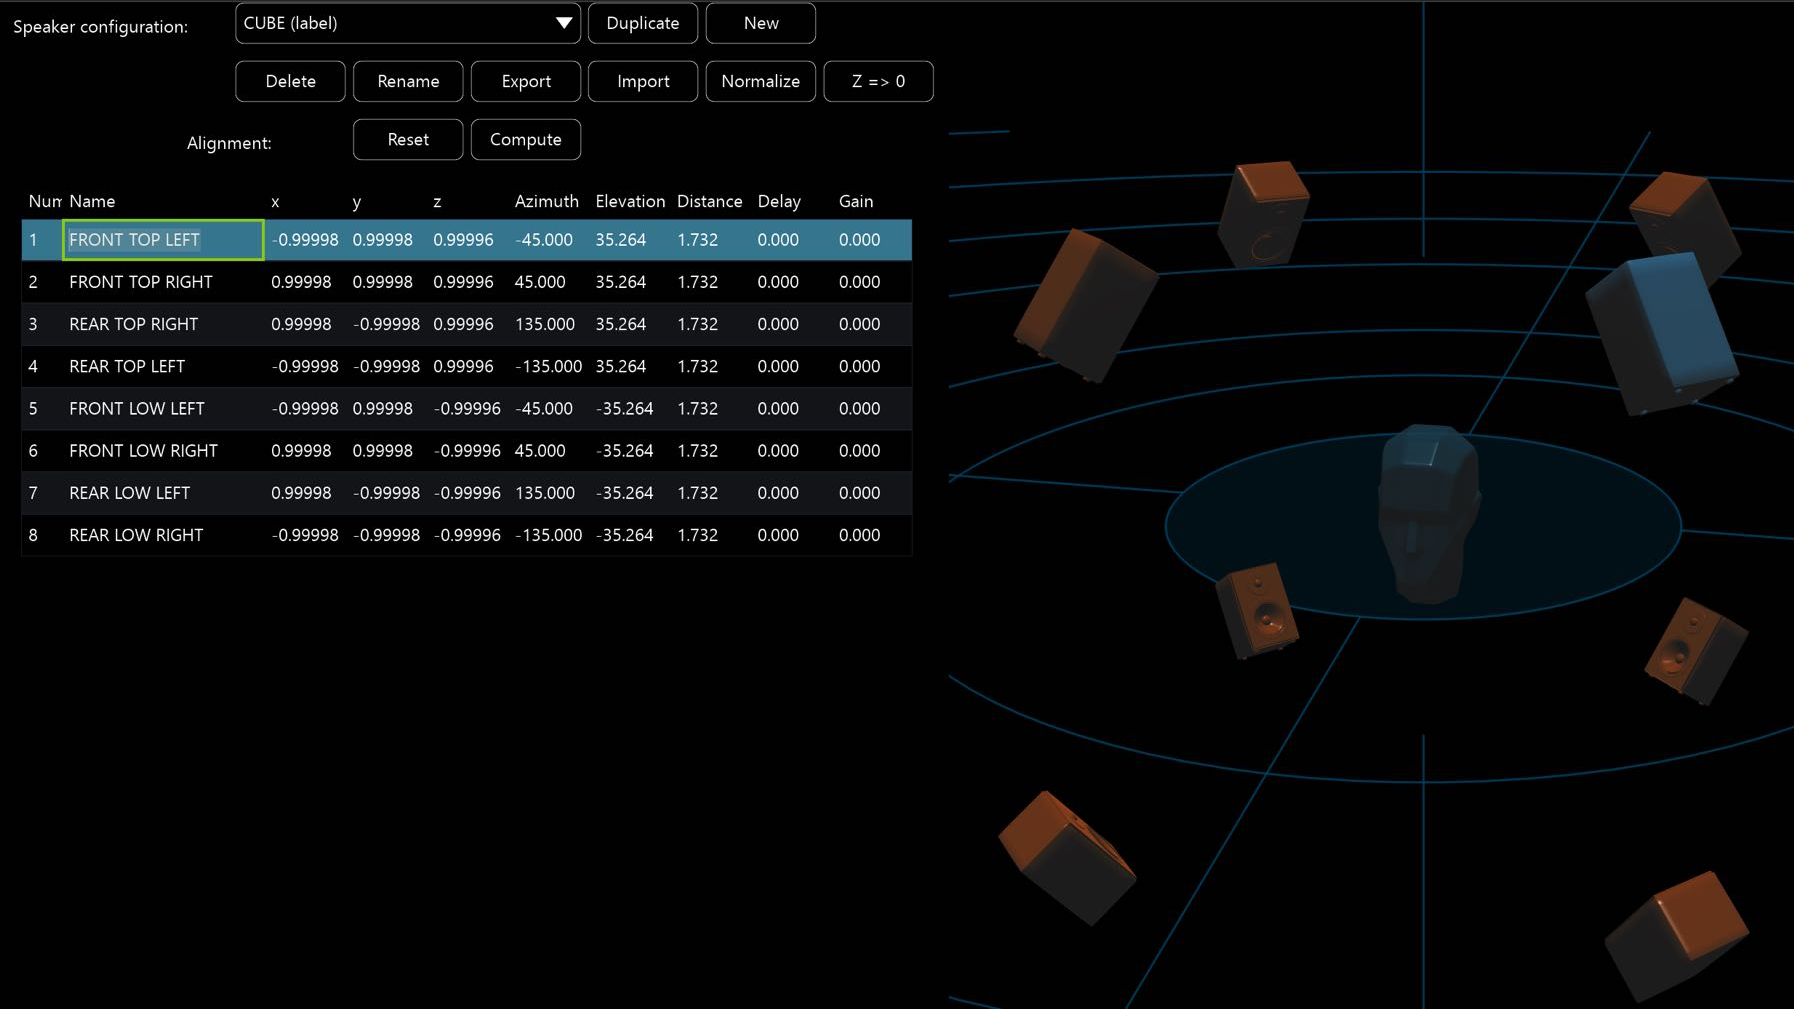
\includegraphics{index_files/mediabag/SpeakerEditor2.png}

The process of matching the correct channel to the correct speaker is
absolutely vital to the successful rendering of the spatial composition
from a \emph{SPAT Revolution} \emph{Virtual Room} into a physical space.
Further critical points to a successful project are the choice of
panning type in a \emph{Virtual Room} and consideration of the
\emph{Sweet Spot} for listener positioning. As it is such an important
and often misunderstood idea, let us take a look at that topic before
going further.

\hypertarget{wave-field-synthesis}{%
\chapter{Wave Field Synthesis}\label{wave-field-synthesis}}

\hypertarget{introduction-1}{%
\section{Introduction}\label{introduction-1}}

Wave Field Synthesis, also known as WFS, is a technique for spatial
audio reproduction. Unlike most of the traditional spatialization
techniques, this technique \textbf{does not} depend on a phantom sound
source (ie: the stereophonic principles allowing the creation of an
acoustical illusion) to recreate an acoustic space.

WFS aims to reproduce the true physical attributes of a given sound
field (the waves front) over an extended area of the listening room.
\textbf{This approach relies on delay and amplitude differences.}

The goal of WFS is to recreate the wavefront of a primary (or virtual)
source synthesized by a large number of individually driven
loudspeakers. Thus, this strategy implies a sampling of the original
wavefront. This is a direct application of the Huygens' principle, which
states that every point on a wavefront is itself the source of spherical
wavelets, and the secondary wavelets emanating from different points
mutually interfere. The sum of these spherical wavelets forms the
wavefront.

Under certain strict conditions, WFS can create the impression of a
source positioned in front of the speaker system. This zone in front of
a speaker line is referred to as the Focus Zone. That being said, the
criteria are quite drastic to get this effect. Ircam states at least 32
speakers should be used with 15 to 20 cm spacing.

\hypertarget{availability---wfs-add-on-license}{%
\subsection{Availability - WFS Add-on
license}\label{availability---wfs-add-on-license}}

\begin{quote}
Referred to as a panning type in \emph{SPAT Revolution}, the WFS spatial
audio reproduction technique is available with \textbf{the WFS Add-on
license option}, available with Ultimate and Essential version.
\end{quote}

\hypertarget{spat-revolution-implementation-of-wfs}{%
\section{SPAT Revolution implementation of
WFS}\label{spat-revolution-implementation-of-wfs}}

\begin{figure}

{\centering 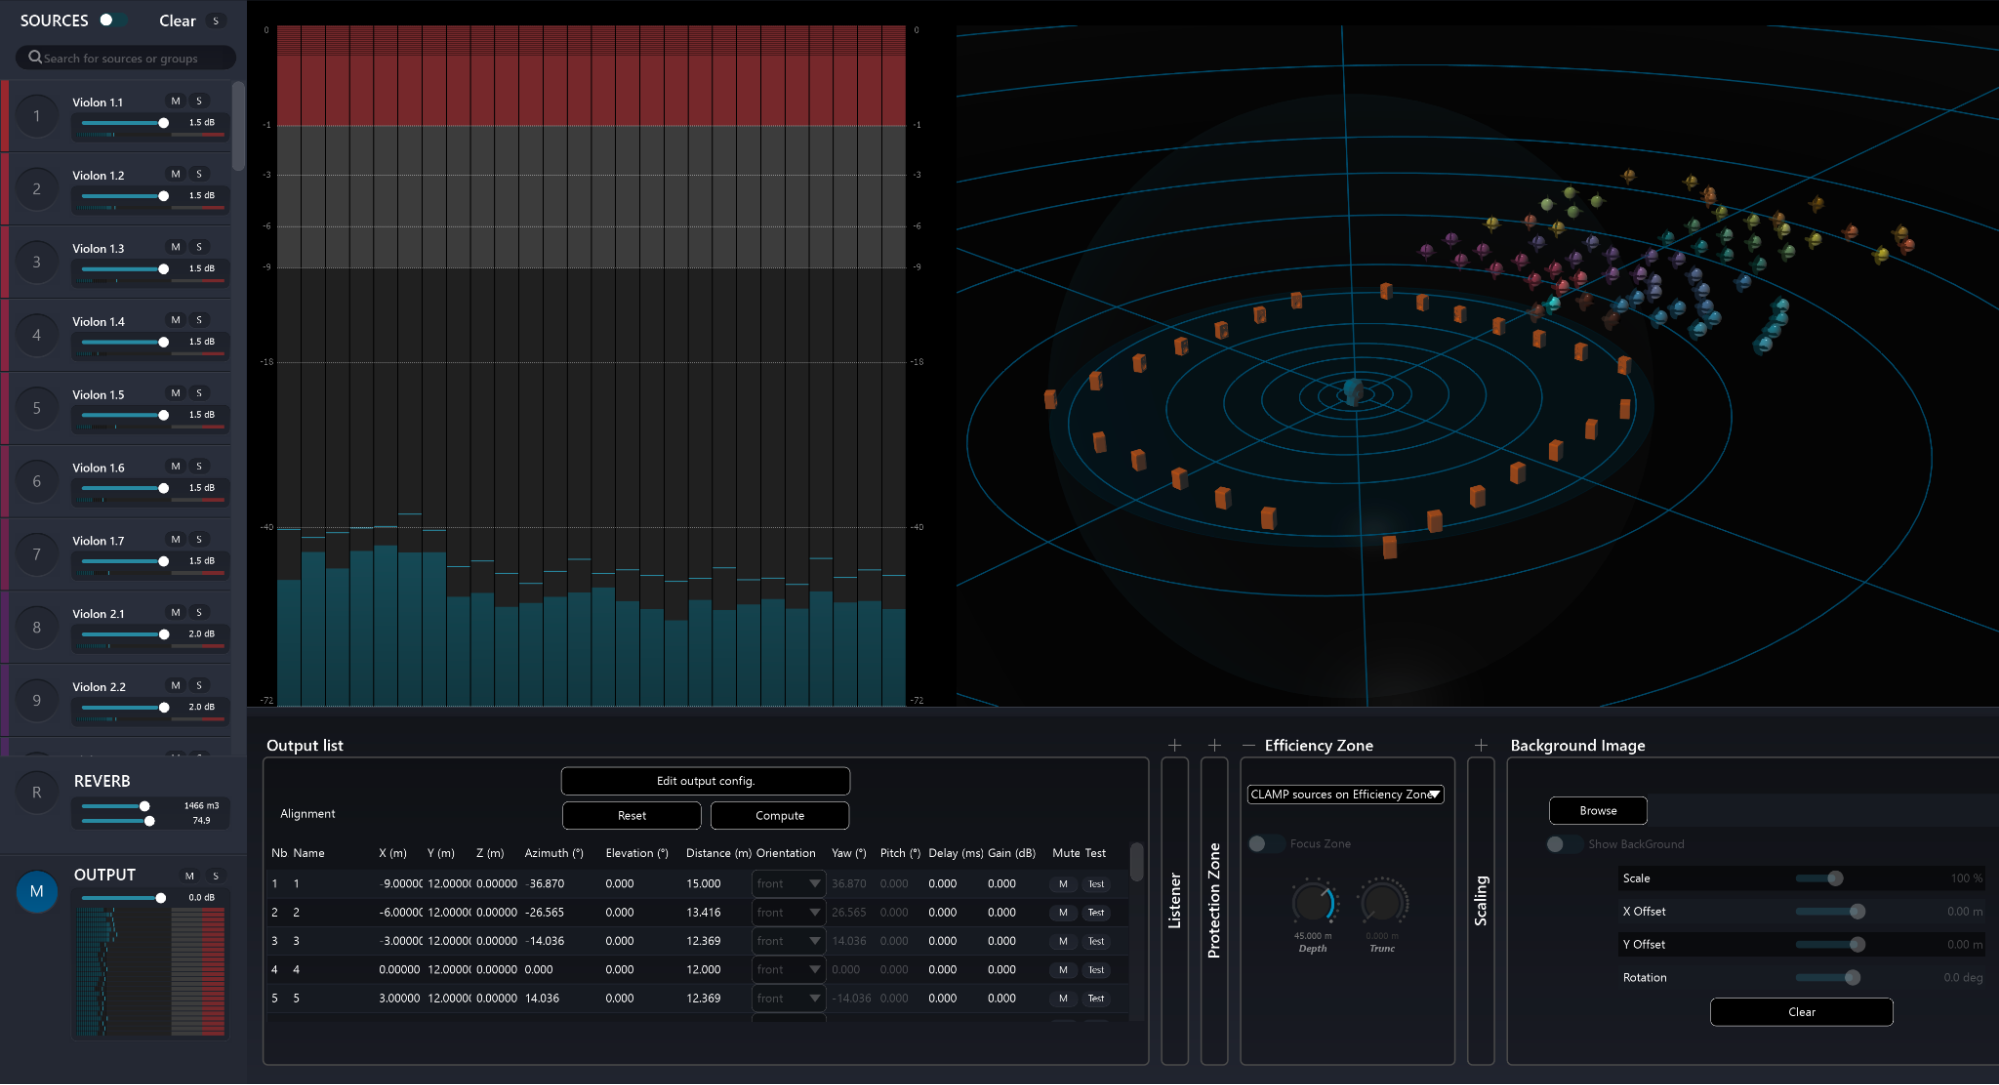
\includegraphics{index_files/mediabag/WFSNiceOutput.png}

}

\caption{WFS}

\end{figure}

Where traditionally WFS is used on a collinear array of very tightly
spaced loudspeakers, SPAT Revolution allows for the use of the spatial
audio reproduction technique on systems with greater spacing, in smaller
loudspeaker quantity and potentially handling any type of 2D or 3D
speaker arrangements.

\begin{figure}

{\centering 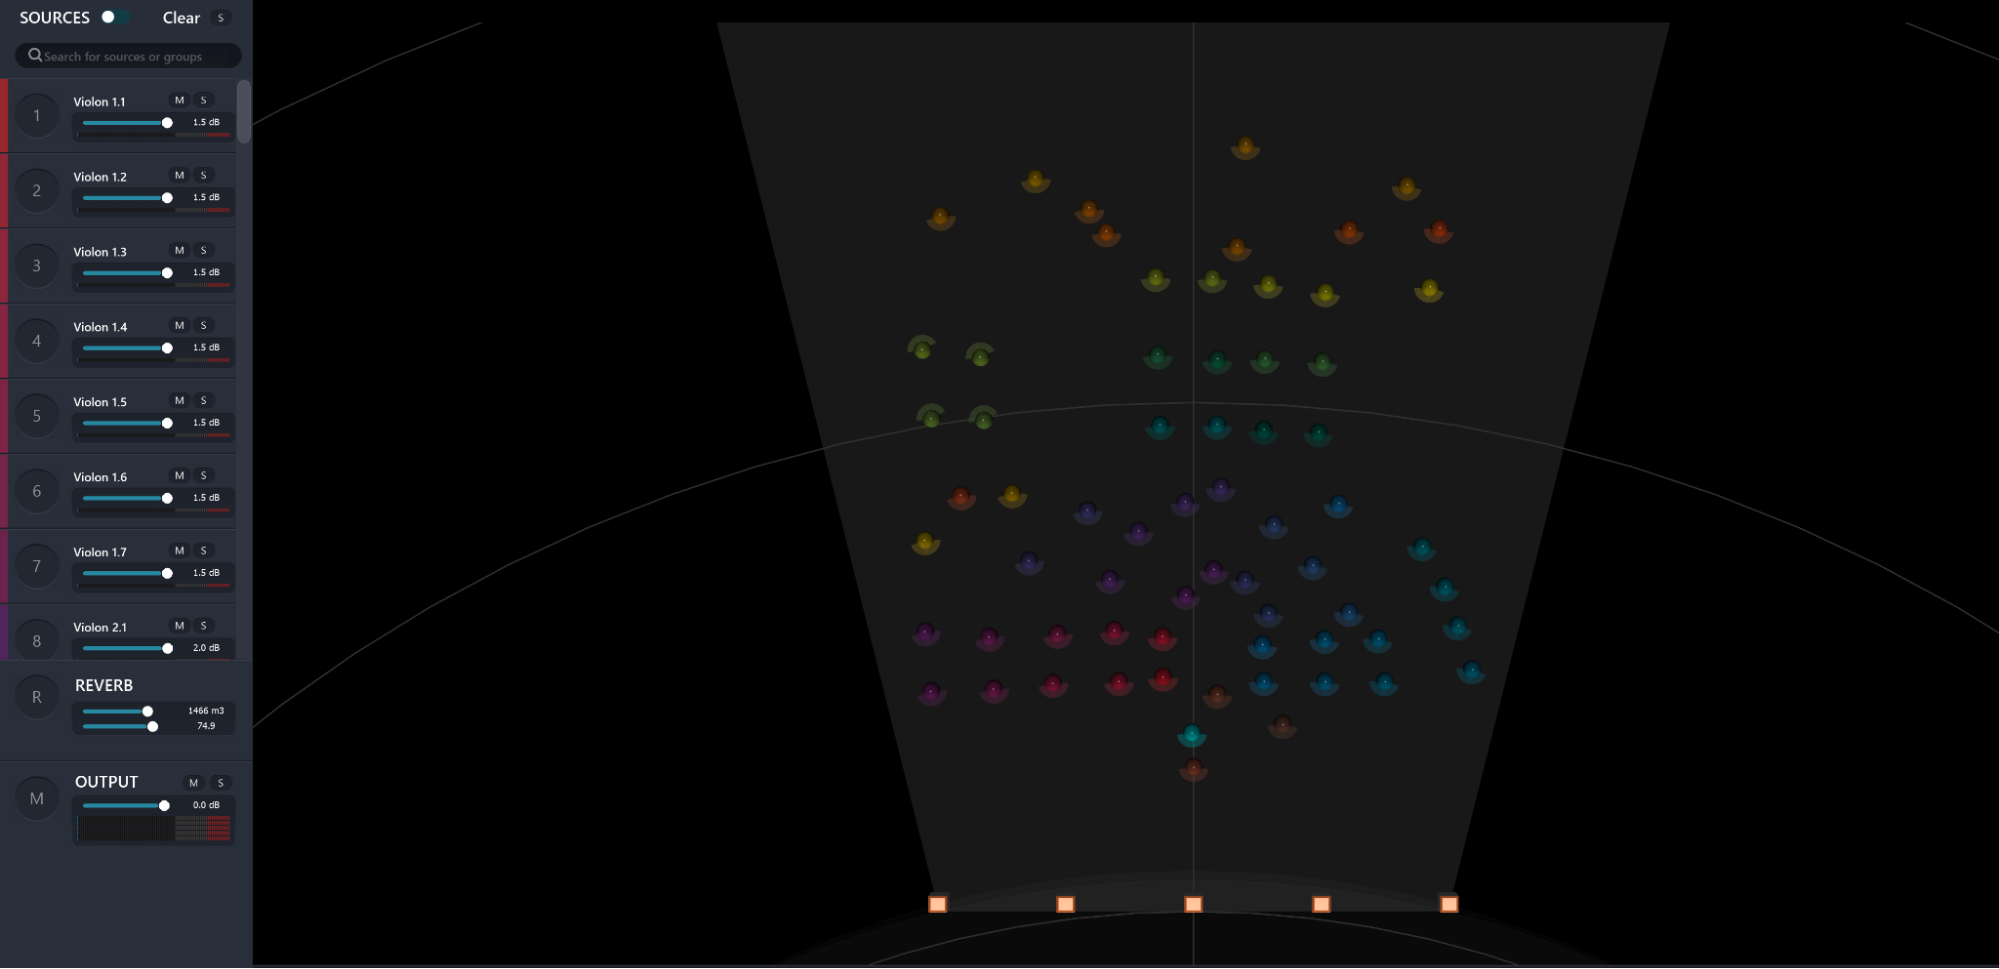
\includegraphics{index_files/mediabag/WFSNice4.png}

}

\caption{WFS}

\end{figure}

The panning method will become available to the room inspector as soon
as a minimum of 5 loudspeakers are available.

!\textgreater{} Even if a large spacing between speakers is allowed,
keep in mind that the greater the spacing you have, the less coherent
the results will be.

\begin{figure}

{\centering 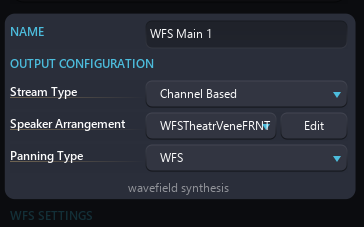
\includegraphics{index_files/mediabag/WFSPanning.png}

}

\caption{WFS Panning type}

\end{figure}

The chosen WFS implementation is a minimum latency approach. This simply
means that the closest speaker to the source has no delay. In the focus
zone, the same principle is used to keep the latency at its minimum.

\hypertarget{focus-zone}{%
\subsection{Focus Zone}\label{focus-zone}}

When using the WFS panning technique on a collinear frontal line
arrangement, the Efficiency zone section in the room output section
provides an option to activate the focus zone, i.e.~the zone in front of
a line of speakers. It is deactivated by default as it is recommended
that a certain density and spacing exist for the speaker arrangement.

!\textgreater{} Enabling this option may trigger an Efficiency zone
warning if the system does not respect the 0.4 meter spacing between
speaker source elements recommendation.

\begin{figure}

{\centering 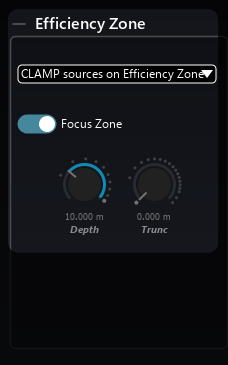
\includegraphics{index_files/mediabag/FocusZoneEnable.png}

}

\caption{Focus zone Enable}

\end{figure}

\begin{figure}

{\centering 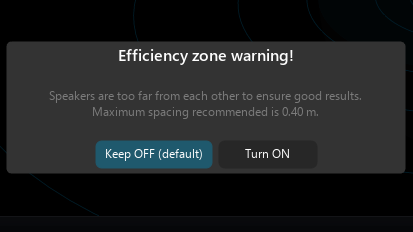
\includegraphics{index_files/mediabag/FocusZoneWarning.png}

}

\caption{Focus zone warning}

\end{figure}

After activating, it will extend the efficiency zone with a focus area
starting at the listening reference thus allowing sources to freely move
inside the listening area.

\begin{figure}

{\centering 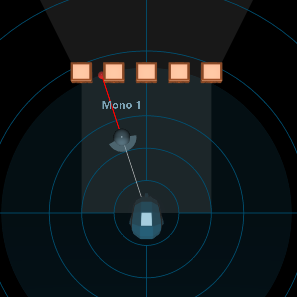
\includegraphics{index_files/mediabag/FocusZone.png}

}

\caption{Focus zone}

\end{figure}

\hypertarget{further-readings}{%
\subsection{Further readings}\label{further-readings}}

\begin{itemize}
\item
  \href{http://www.syntheticwave.de/Wavefieldsynthesis.htm}{Good
  introduction to WFS}
\item
  \href{http://recherche.ircam.fr/equipes/salles/WFS_WEBSITE/Index_wfs_site.htm}{IRCAM
  website on WFS}
\item
  \href{http://recherche.ircam.fr/equipes/salles/WFS_WEBSITE/Documents/WFS_overview.pdf}{Sound
  Scene Creation and Manipulation using Wave Field Synthesis}
\end{itemize}

\hypertarget{wfs-settings}{%
\section{WFS Settings}\label{wfs-settings}}

\begin{figure}

{\centering 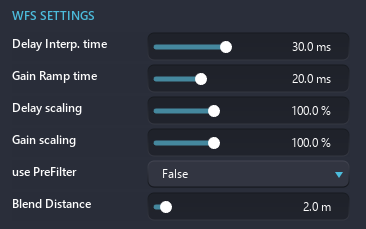
\includegraphics{index_files/mediabag/WFSSettings.png}

}

\caption{WFS Settings}

\end{figure}

FLUX:: WFS implementation uses an interpolation strategy using a very
precise calculation mode for delays values. This is to allow for a
smooth transition with source movement rather than delay steps (inherent
from digital audio). \textbf{6 parameters} are available in the room
inspector of the setup page, and can allow to fine-tune the WFS render

\textbf{Delay interp. time:} The delay interpolation time is the time it
will take to go from one delay value to another delay value. In WFS,
interpolation time allows a smooth transition when a source is moved.
Depending on your source content, and your scene movements, you may find
this setting useful to modify.

\textbf{Gain ramp time:} Similar to the concept of delay interpolation
time, the gain ramp time is the time it will take to transition from one
set of gain values to another.

\textbf{Delay scaling:} This parameter allows scaling the computed
delays for all sources. It allows shaping the wavefront. Setting the
delay scaling at 0\% will set all delays to 0 ms, only the amplitude
differences will remain.

\textbf{Gain scaling:} This parameter allows scaling of the computed
gains for all sources. It is really useful on close WFS line, in order
to spread the audio content all along the line or speaker setup, for
front-fills for example. For example, you can decrease the percentage in
order to activate more loudspeakers serving well audience sitting close
to the loudspeaker line.

\textbf{use PreFilter:} A spectral correction in WFS systems called
Pre-equalization. This parameter enables/disables a low-shelf filter in
order to compensate for the low frequencies boost created by the speaker
antenna.

\textbf{Blend distance:} A 2.0-meter distance behind the speaker line is
defined by default providing a transition zone as sources get closed to
speakers and can help prevent some artifacts.

\hypertarget{scene-based-streams}{%
\chapter{Scene based streams}\label{scene-based-streams}}

\hypertarget{introduction-to-ambisonics}{%
\section{Introduction to Ambisonics}\label{introduction-to-ambisonics}}

Simply put: Ambisonics is a specific method for creating, capturing and
playing back spatial audio. It is radically different from other
surround techniques as the technology is capable of reproducing a
spherical representation of sound where the directional information of a
source is located in a 3D soundfield.

Ambisonic is also both a recording and a spatial synthesis technique,
where one can capture the full environment in 3D sound through the use
of so called A-Format microphones such as the: Soundfield SPS200, Røde
NT-SF1, Sennheiser Ambeo, Coresound TetraMic and more. Alternatively, a
sound field can be synthesized from any mono, stereo and multichannel
sources to Ambisonics, constructing a virtual 3D sound environment by
placing the sources at locations in a virtual 3 dimensional field.

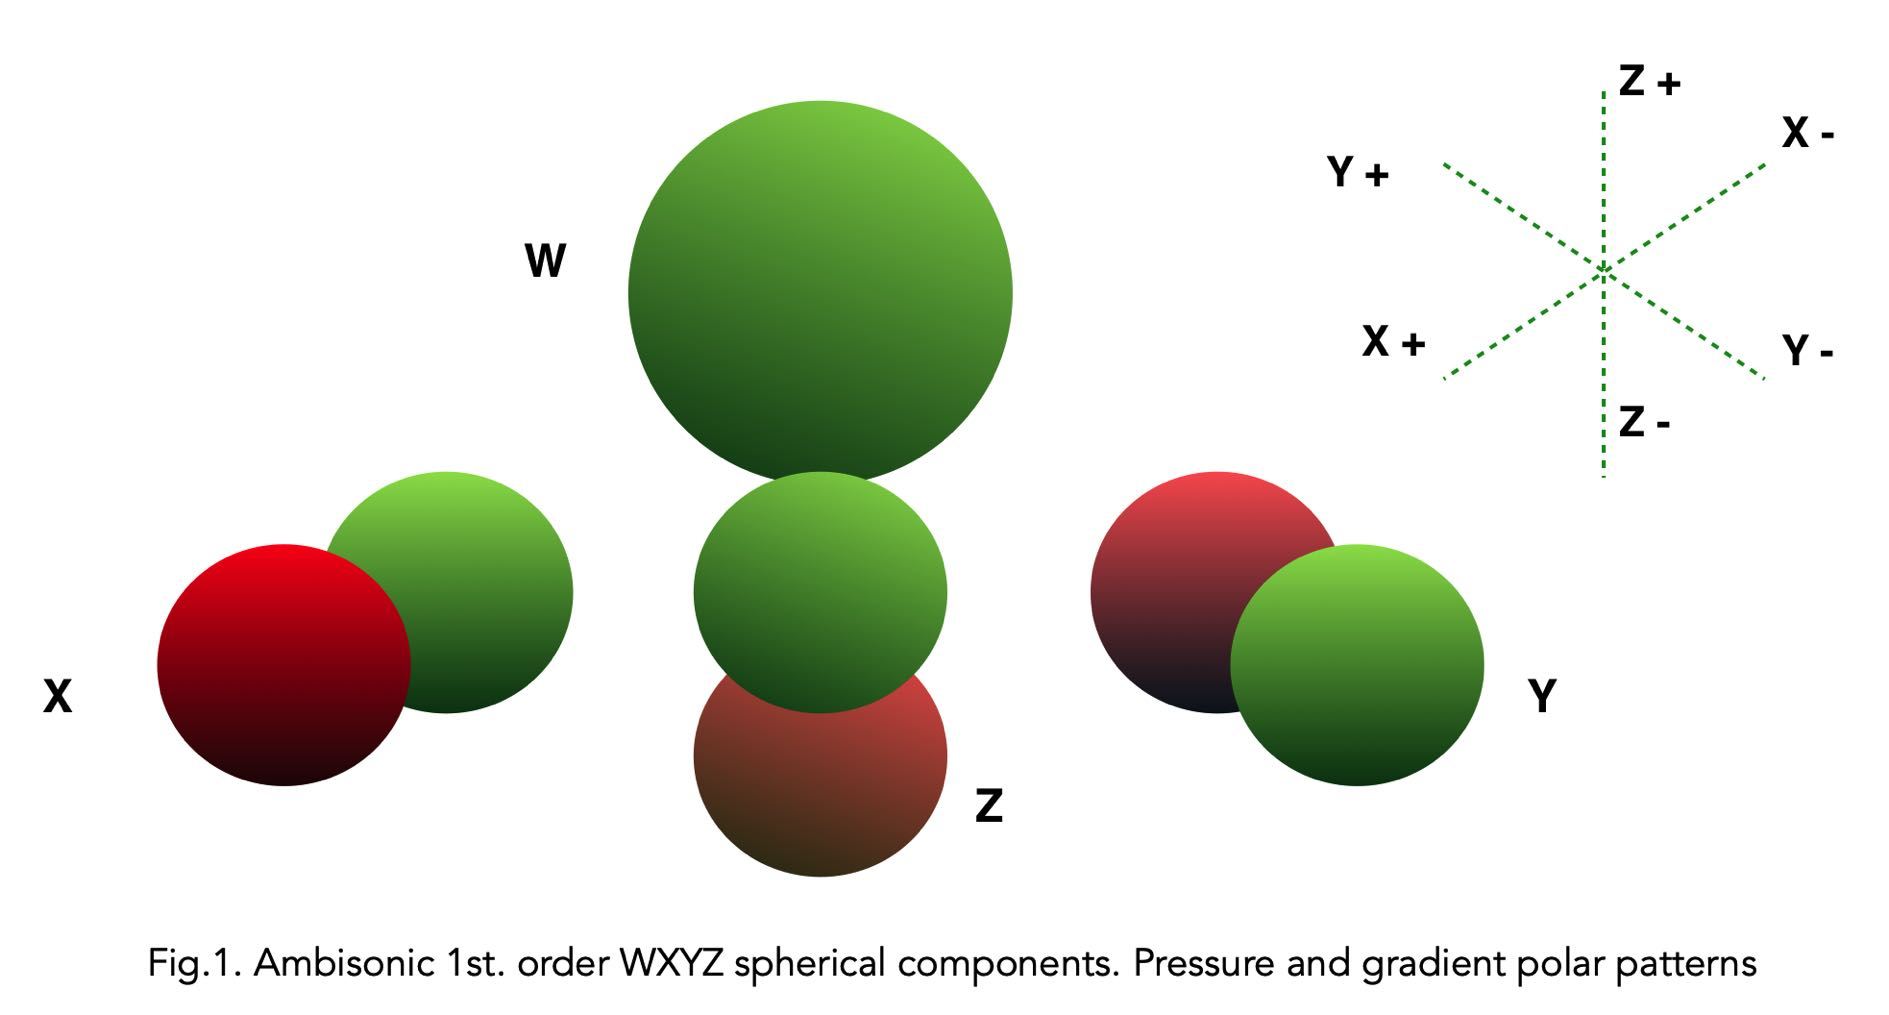
\includegraphics{index_files/mediabag/Ambisonic.png}

\hypertarget{encoded-audio}{%
\section{Encoded audio}\label{encoded-audio}}

Ambisonic, as opposed to other surround and spatial techniques and
methods does not carry a speaker signal. It is an \textbf{encoded} audio
signal that has to be \textbf{decoded} to listen on speakers. This
encoding / decoding scheme has the advantage of being very portable and
flexible since one is not tied to a specific speaker setup. i.e., you
can have your ambisonic mix played on a number of speaker setups, for
instance quad, headphones (binaural), 5.1, 6, 8, 7 speakers, etc. based
on the chosen decoder.

When Ambisonics is played back on speakers, all the speakers contribute
to the directional content, what one is hearing is not the sound coming
from a specific speaker but from a specific direction.

\includegraphics{index_files/mediabag/ReaperHOA3DTrack.jpg}

\begin{quote}
Overview of a fifth-order HOA 3D Ambisonic File created by Tine Surell
Lange.
\end{quote}

\hypertarget{order}{%
\section{Order}\label{order}}

Ambisonics is a technology that encodes sound sources along with
full-sphere positional information, as complex interleaved audio files
that need decoding before they can be listened to on speakers. The
lowest order, order 1, and the simplest form of 3D Ambisonics require 4
channels, conventionally named as:

\begin{itemize}
\tightlist
\item
  \textbf{W} (mono sum)
\item
  \textbf{X} (X-axis information)
\item
  \textbf{Y} (Y-axis information)
\item
  \textbf{Z} (elevation information)
\end{itemize}

The 4 channels or spherical components W, X, Y and Z can also be
described as the pressure patterns found in an omni-microphone (W) and
three figure-of-8 microphones for left/right (Y), front/back (X) and
up/down (Z) as depicted in the above figure.

High Order Ambisonics (HOA) needs more channels to contain the complex
interleaved Ambisonics domain information. The components' count
increases with the order: WXYZUVSTRPQNOLMK\ldots{} High Orders encode
and decode into sharper and more accurate spatial information as the
Order gets higher - but the number of channels needed to hold all the
`spherical harmonics' along with the serious computation involved
increases quickly.

3D full sphere HOA channel counts are defined by the function (n+1)\^{}2
(where n is the Ambisonic Order).

\begin{itemize}
\tightlist
\item
  1st Order 3D -\textgreater{} 4 Channels
\item
  2nd Order 3D -\textgreater{} 9 Channels
\item
  3rd Order 3D -\textgreater{} 16 Channels
\item
  4th Order 3D -\textgreater{} 25 Channels
\item
  5th Order 3D -\textgreater{} 36 Channels
\item
  6th Order 3D -\textgreater{} 49 Channels
\item
  7th Order 3D -\textgreater{} 64 Channels
\end{itemize}

\emph{Ambisonics} can also be encoded without elevation - this is called
2D horizontal and is quite suitable for decoding to configurations that
do not have speakers on elevated planes. The 2 dimensional Ambisonic
data is encoded in multichannel files with a channel count defined by
the function 2n+1 (where n still is the Ambisonic order.

\begin{itemize}
\tightlist
\item
  1st Order 2D -\textgreater{} 4 Channels
\item
  2nd Order 2D -\textgreater{} 5 Channels
\item
  3rd Order 2D -\textgreater{} 7 Channels
\item
  4th Order 2D -\textgreater{} 9 Channels
\item
  5th Order 2D -\textgreater{} 11 Channels
\item
  6th Order 2D -\textgreater{} 13 Channels
\item
  7th Order 2D -\textgreater{} 15 Channels
\end{itemize}

!\textgreater{} With \textbf{Essential} license, 1st, 2nd and 3rd orders
are only available.

\hypertarget{normalization-sorting-and-presets}{%
\section{Normalization, sorting and
presets}\label{normalization-sorting-and-presets}}

These different components are organised according to different
standards, known as sorting. The three most used are available in
\emph{SPAT Revolution}: - ACN: Ambisonic Channel Number,
WYZXVTRSUQOMKLNP\ldots{} - SID: Single Index Designation,
WXYZUVSTRPQNOLMK\ldots{} - FMH: Furse-Malham Harmonics,
WXYZRSTUVKLMNOPQ\ldots{}

Different normalizations exist also with ambisonics. This normalization
defines the relative level of the omni component compared to the other
channels. It differs according to the dimension of the Ambisonics: -
SN2D/SN3D: Schmidt-Seminormalized. - N2D/N3D: Fully-Normalized. - FuMa:
Furse-Malham normalization.

To help with these different standards, we have created Ambisonics
presets to simplify the use of it. These setups the normalization and
sorting with common standards: - AmbiX: used for example by Youtube and
Facebook 360. The normalization is SN2D / SN3D and the sorting ACN. -
B-Format: the normalization is Fuma, and the sorting FMH. - SPAT Room:
the normalization is N2D / N3D and the sorting ACN.

!\textgreater{} Do not forget to transcode the ambisonic input if the
format is different from N2D/N3D and ACN.

\hypertarget{a-format}{%
\section{A-Format}\label{a-format}}

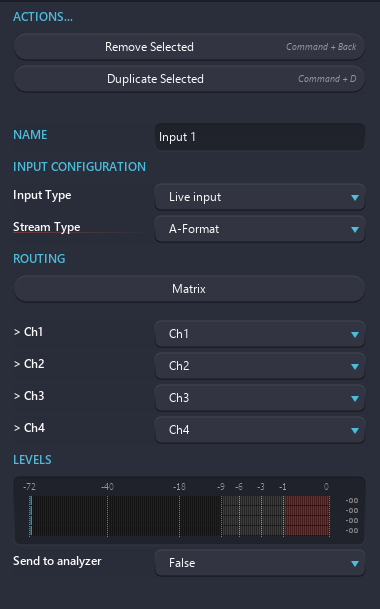
\includegraphics{index_files/mediabag/InputInspectorAFormat.png}

A-format is a 4-channel audio stream. It is the RAW output of a
first-order ambisonic microphone, so it has not been encoded to
ambisonic yet. So we need to transcode a A-Format input to an HOA or a
channel-based stream. Because each manufacturer has their own strategy
to create such microphone, we have almost as many transcoder as A-format
microphone builder. \emph{SPAT Revolution} comes with a comprehensive
list of A-Format transcoder, including Sennheiser Ambeo, Soundfield,
DPA, Oktava etc.

\hypertarget{history-and-references}{%
\section{History and references}\label{history-and-references}}

Ambisonics was originally developed by the late British mathematician
and sound engineer Michael Gerzon and others in the 1970s. Although it
was a commercial failure at the time, this very powerful spatial
technique has since been advanced greatly by a number of composers,
sound designers and researchers. With the introduction of Virtual
Reality, fast decoders and related technology, Ambisonics is getting a
new renaissance being a perfect format for such applications.

If you want to learn more about Ambisonics and its mathematical
foundation here are some good starting points:

\begin{itemize}
\tightlist
\item
  \url{https://www.researchgate.net/publication/280010078_Introduction_to_Ambisonics}
\item
  \href{https://en.wikipedia.org/wiki/Ambisonic_data_exchange_formats}{Wikipedia
  article about normalization and sorting}
\item
  \href{https://link.springer.com/book/10.1007/978-3-030-17207-7}{Frank
  Zotter' book about Ambisonics}
\end{itemize}

\hypertarget{ambisonic-transcoding}{%
\chapter{Ambisonic Transcoding}\label{ambisonic-transcoding}}

\hypertarget{default-transcoding}{%
\section{Default transcoding}\label{default-transcoding}}

When patching an HOA or B-Format input to a source, or a HOA room to a
channel-based output, a transcoder will be automatically inserted. This
transcoder will, by default, be set to the Ring or Sloane speaker
arrangement corresponding to the HOA order, and, will select an AllRad
decoder.

\begin{quote}
Ring and Sloane are uniform setups which are recommended for optimized
transcoding. I will guarantee a precise localization, in particular when
transcoding an ambisonic input in order to use it in a room.
\end{quote}

\hypertarget{transcoding-method}{%
\section{Transcoding method}\label{transcoding-method}}

\hypertarget{projection}{%
\subsection{Projection}\label{projection}}

Projection decoding is also sometimes called ``sampling ambisonic
decoding'' (SAD). It is the simplest form of ambisonic decoding. It
samples the virtual panning function at the loudspeaker directions. SAD
is optimal for loudspeakers arranged as t-design layouts, with t ≥
(2N+1) ( N being the Ambisonics order). Typically, the SAD should only
be used for 2D loudspeaker layouts, i.e., regularly arranged in a
circle. Avoids this decoder for 3D setups.

\emph{What is a T-Design Layout?}

To keep it really simple, t-design is a mathematical way of constructing
sphere perimeters or circle surfaces with an array of point that is
homogenous. In 2D the point simply put on a circle and are evenly
spaced. In 3D, things get much more complicated many t-design point
layouts exist. In \emph{SPAT Revolution}, we chose to use the method
used by the mathematician Sloane for our speaker layouts.

\hypertarget{regularized-pseudo-inverse}{%
\subsection{Regularized
pseudo-inverse}\label{regularized-pseudo-inverse}}

The pseudo-inverse decoder, or ``mode-matching decoder'' (MMAD), is
suitable for both 2D and 3D. It is based on a pseudo-inverse of the
re-encoding matrix. MMAD is well-behaved for regular loudspeaker
arrangements. It can also give good results with slightly irregular
setups. However, it can become unstable with strongly irregular setups,
i.e., it can completely blow up the speaker feeds. So, be careful.

The regularized pseudo-inverse decoder or ``regularized-mode-matching
decoder'' (RMMAD) is somehow similar to MMAD. However, it uses a
regularization factor for stabilization of the pseudo-inverse. This
regularization factor (alpha) varies from 0\% to 100\%. A value of 0\%
provides results similar to MMAD. A value of 100\% generates even energy
distribution, i.e., results similar to EPAD. Intermediate values of
alpha allow to ``blend'' MMAD and EPAD.

\hypertarget{energy-preserving}{%
\subsection{Energy preserving}\label{energy-preserving}}

EPAD (energy preserving ambisonic decoding) and AllRAD (All-round
Ambisonic decoding) are other HOA decoding methods suitable for 2D and
3D HOA, and they can cope with any kind of loudspeaker arrangement.
These decoding methods always work, as soon as there are enough
loudspeakers; they are always feasible and by nature numerically stable.
EPAD uses a regularized matrix inversion such that the decoded energy is
preserved even with non-uniformly arranged arrays (and even for
directions with only sparse loudspeaker coverage). EPAD is the default
method in spat5 (and the one we usually recommend).

\hypertarget{allrad}{%
\subsection{AllRAD}\label{allrad}}

``All-round Ambisonic decoding'' (AllRAD) is designed in two steps.
First, an optimal virtual loudspeaker layout using t-design arrangement
is considered (for which the SAD is optimal). Secondly, the signals of
these virtual loudspeakers are mapped to the real loudspeakers via VBAP.

\hypertarget{improved-allrad}{%
\subsection{Improved AllRAD}\label{improved-allrad}}

``Improved All-Round Ambisonic Decoding'' (AllRAD+) combines AllRAD and
SAD. Constant energy that is achieved for the idealized virtual
loudspeaker setup in AllRAD is corrupted by the VBAP stage as, per
loudspeaker pair, all virtual sources are superimposed linearly instead
of energetically. The prevailing linear superposition increases the
energy wherever the loudspeaker spacing is large. Roughly, at such
directions AllRAD doubles the energy, whereas it is halved at directions
with dense loudspeaker spacing. Conversely, SAD might lose all energy
where the loudspeaker spacing is large and roughly doubles it where the
loudspeaker spacing is dense. AllRAD+ tries to solve this issue by
combining (i.e., mixing) SAD and AllRAD. The loudness variation of
AllRAD+ is competitive with EPAD and its angular mapping resembles
AllRAD.

\hypertarget{transcoding-types}{%
\section{Transcoding types}\label{transcoding-types}}

To improve the ambisonic render, there are some strategies that can be
applied at the decoding stage. The idea is to optimize the phase or the
energy to improve the sound localization.

\hypertarget{basic}{%
\subsection{Basic}\label{basic}}

This is the standard way to decode ambisonic, and no optimization is
applied.

\hypertarget{inphase}{%
\subsection{InPhase}\label{inphase}}

The audio content will be optimized in phase for the all spectrum.

\hypertarget{maxre}{%
\subsection{MaxRe}\label{maxre}}

The energy of the audio content will be optimized, for the all spectrum.

\hypertarget{basicmaxre}{%
\subsection{BasicMaxRe}\label{basicmaxre}}

The low end of the audio content is not optimized, but a MaxRe method is
applied to the high end. The crossover frequency is by default set to
700~Hz.

\hypertarget{maxreinphase}{%
\subsection{MaxReInPhase}\label{maxreinphase}}

The low end of the audio content is optimized in energy (MaxRe), but a
in phase method is applied to the high end. The crossover frequency is
by default set to 700~Hz.

\hypertarget{inphasemaxre}{%
\subsection{InPhaseMaxRe}\label{inphasemaxre}}

As phase optimization is more efficient in the low frequencies, and
energy optimization is prominent in the high frequencies, this method
takes this phenomenon to its advantage by splitting the signal in two
frequency bands. The crossover frequency is by default set to 700~Hz and
can be adjusted.

\part{SPAT Environment}

This section will go through the \emph{SPAT Revolution} software
environment in more detail. We will step through each of the main
Graphic Editor views.

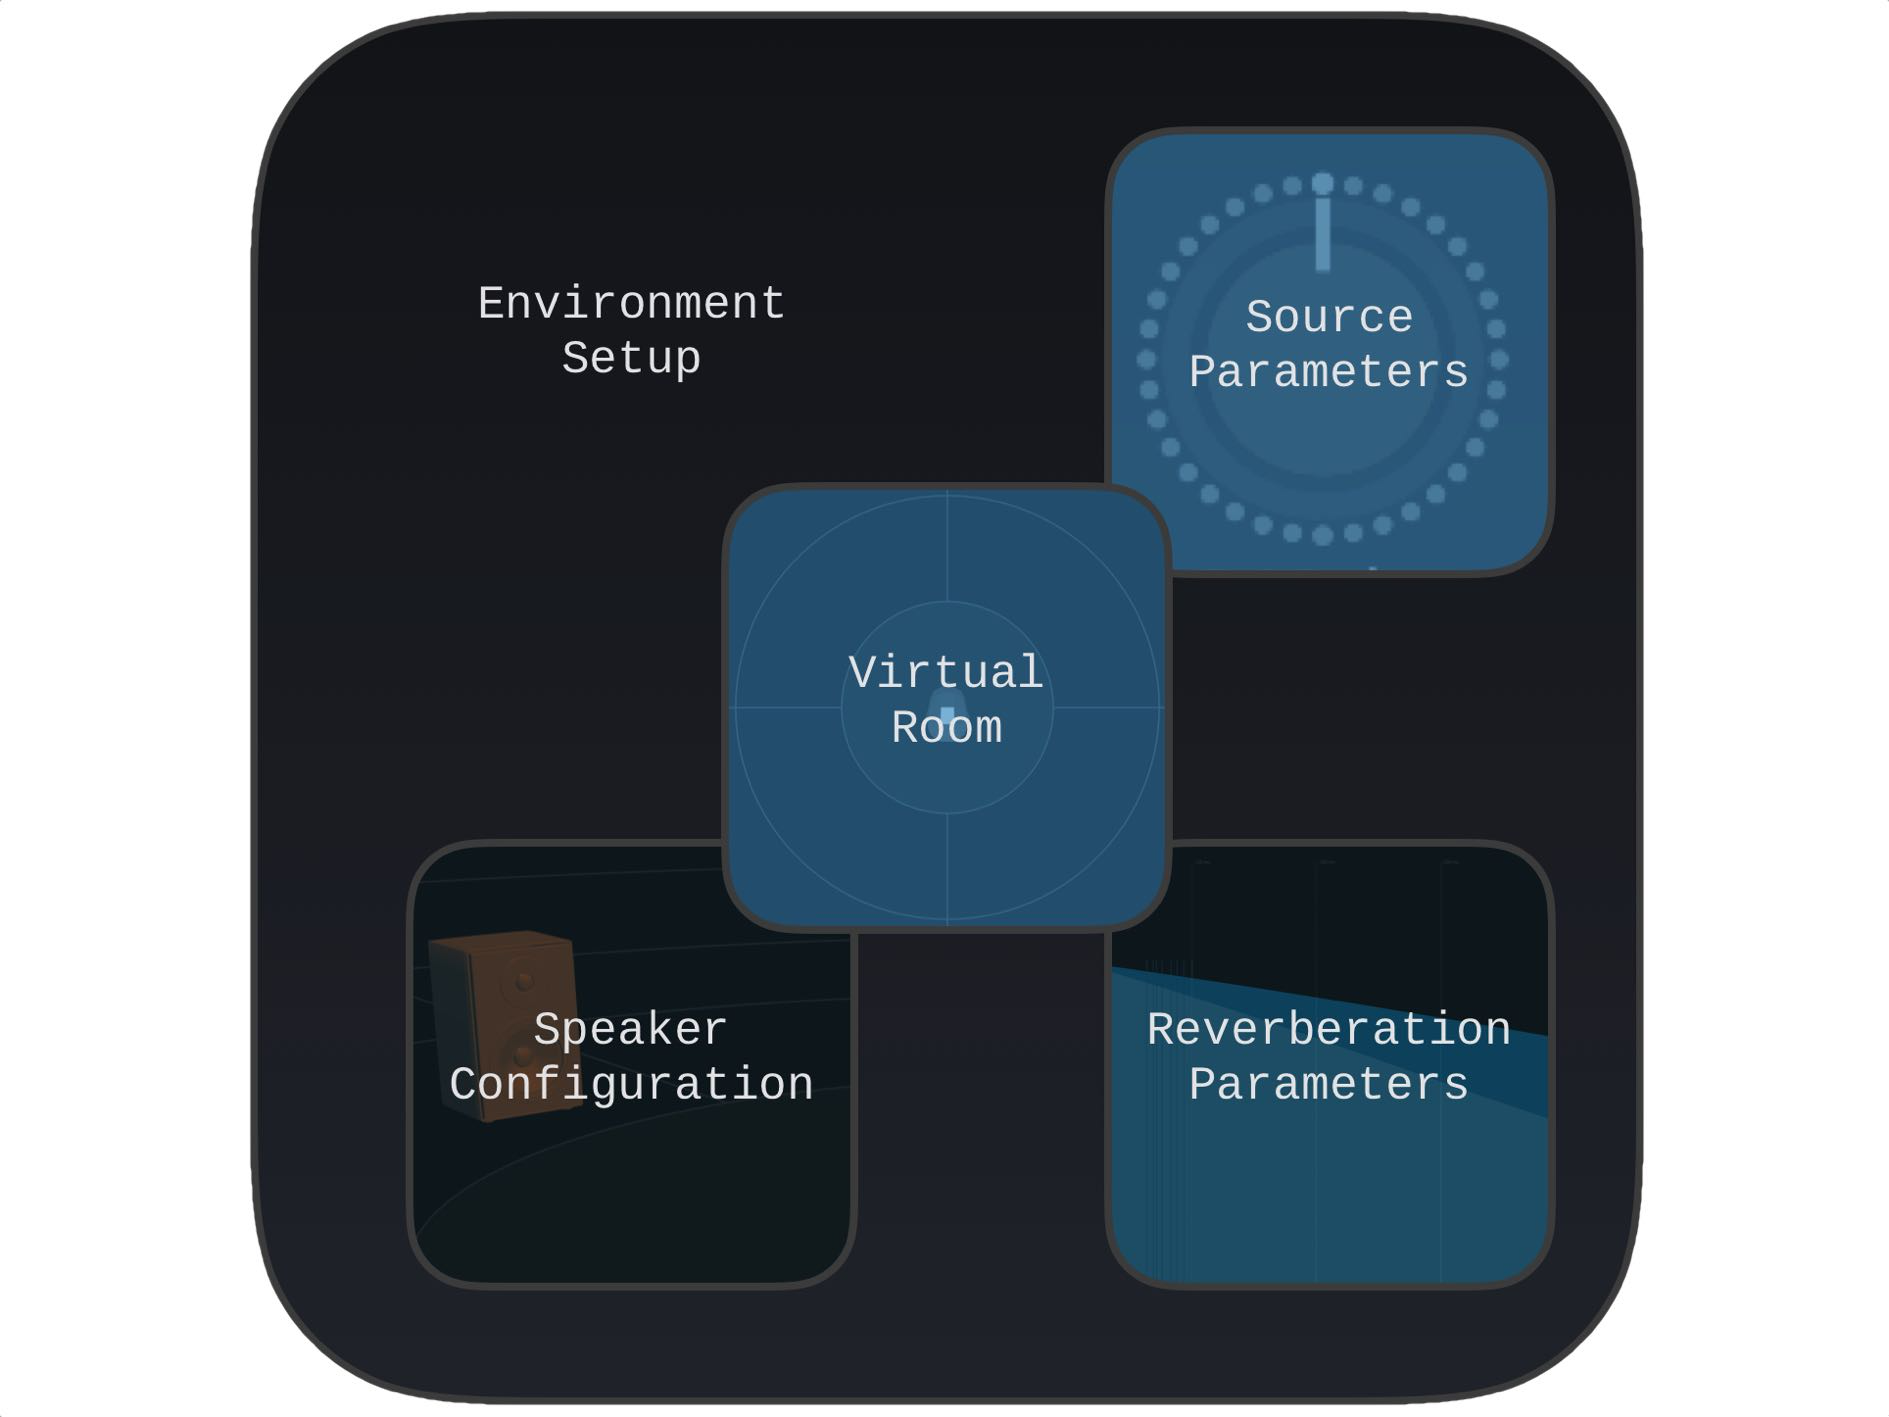
\includegraphics{index_files/mediabag/Environment.png}

\textbf{Rendering to Speakers}

In order for the virtual scene to translate correctly as an immersive
sound experience in a speaker format, SPAT needs to have an accurate
model of a \emph{multichannel speaker arrangement} which will be used to
map the multichannel information to the destination speakers and render
the sound field correctly in a real space. To this end, you will find a
large library of standard and specialized speaker arrangements already
built into SPAT which can be used in various places throughout the
\textbf{Environment Setup}.

Speaker configurations can be used to fit the format of a virtual room
to match the actual speaker system being used to diffuse the mix in a
real room. Channel based speaker configurations can also be used to
transcode the format of a virtual source into a virtual room. More about
this later.

The golden rule when working with multichannel based audio is that you
must be sure to choose \emph{exactly} the right formats, speaker
arrangements and channel routing throughout; otherwise the virtual space
will not map correctly into a physical space.

\textbf{Virtual and Real Diffusion}

Successful diffusion of a sound field in space relies on every
loudspeaker being assigned correctly to each software rendered output
channels.

A diffusion system could range from a simple pair of headphones to a 18
(\textbf{Essential}) or unlimited (\textbf{Ultimate}) speakers array and
anything in between. In some of the more virtualized workflows of
\emph{SPAT Revolution}, you may even be thinking about diffusion in a
virtual space on configurations of virtual speaker arrangements and
channel based formats. The same rule for successful diffusion applies
here---the diffusion in the virtual room will be compromised and sound
off if the channel assignments to the virtual systems are incorrect.

In the above illustration, a virtual 5.1 and a virtual Cube arrangement
exist together in a High Order Ambisonic Room, which may eventually be
rendered to some other channel based end format.

\hypertarget{home-page}{%
\chapter{Home Page}\label{home-page}}

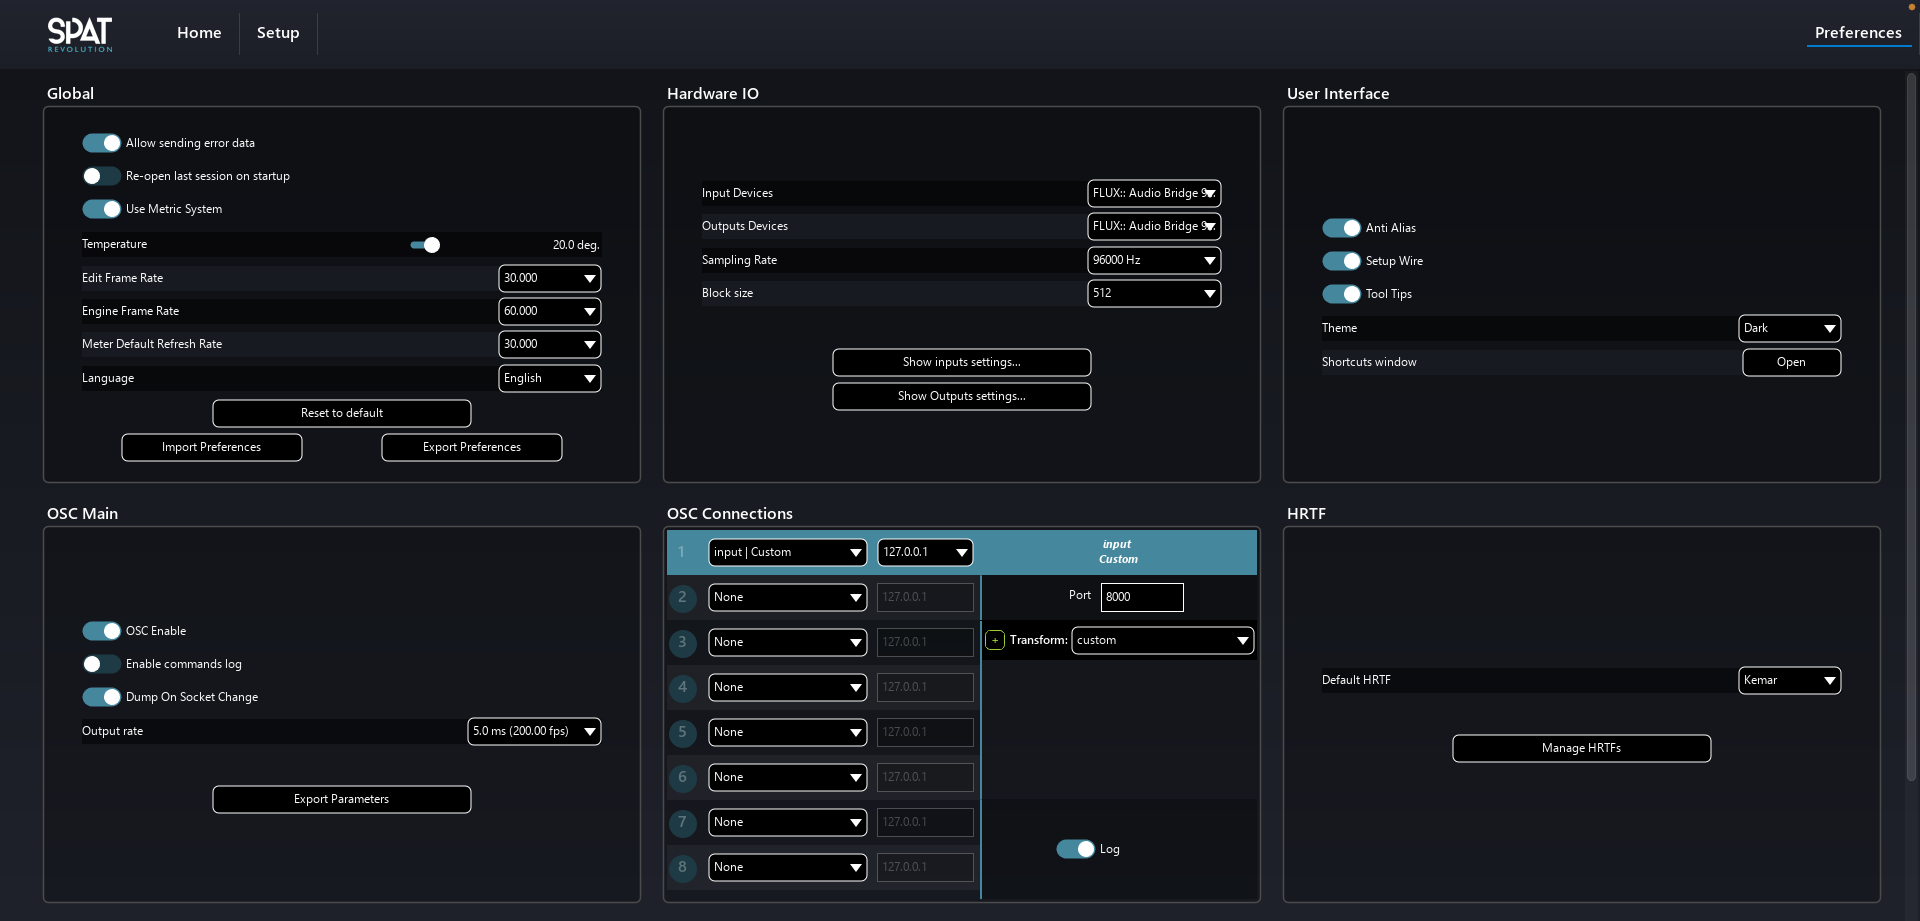
\includegraphics{index_files/mediabag/Page1.png}

This page is the welcome page of \emph{SPAT Revolution}. Here you can
create sessions, open ones from disk or from a list of recent ones or
access to the resources of \emph{SPAT Revolution}.

\hypertarget{welcome-box}{%
\section{Welcome box}\label{welcome-box}}

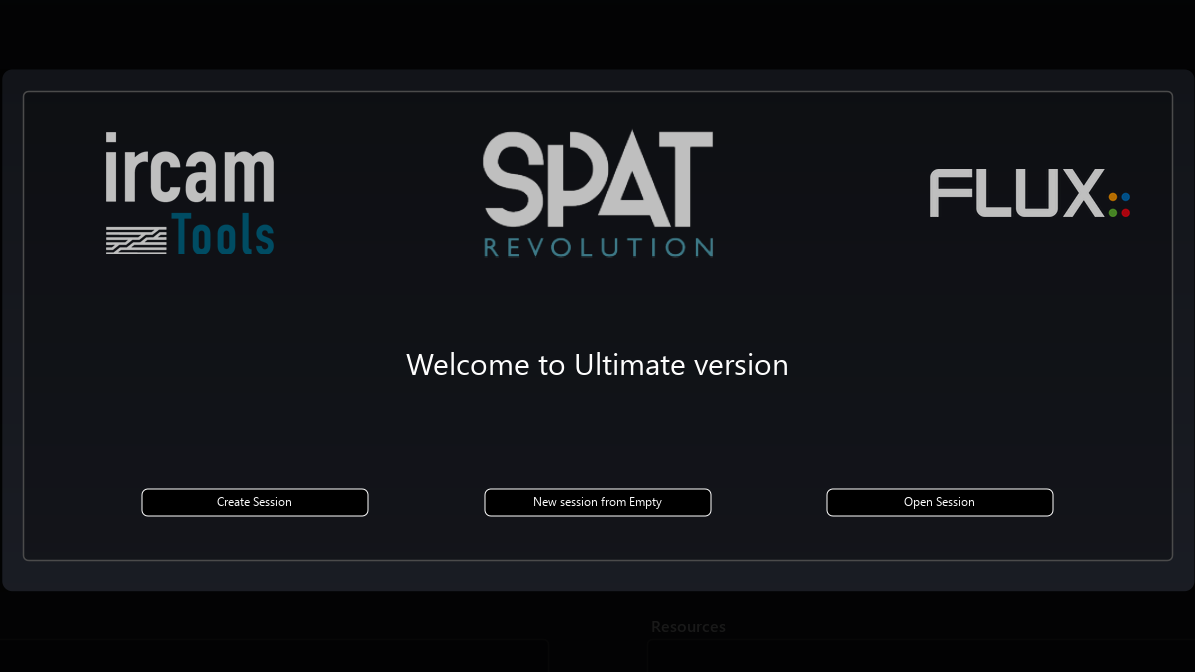
\includegraphics{index_files/mediabag/WelcomeUltimate.png}

This simple box lets you access to basic action of session management.

\hypertarget{create-session}{%
\subsection{Create Session}\label{create-session}}

Create a session with a wizard to set up the routing.

\hypertarget{new-session-from-empty}{%
\subsection{New session from empty}\label{new-session-from-empty}}

Create an empty session, without calling the wizard.

\hypertarget{open-a-session}{%
\subsection{Open a session}\label{open-a-session}}

Let you open a session from a disk.

\hypertarget{recent-sessions}{%
\section{Recent Sessions}\label{recent-sessions}}

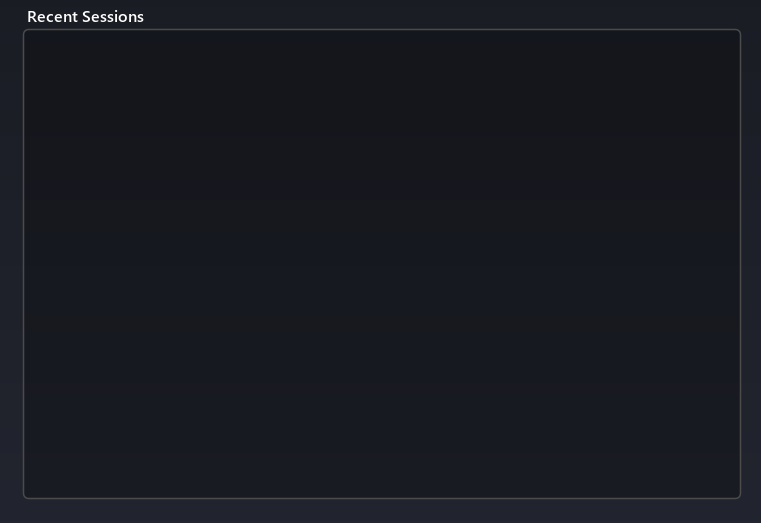
\includegraphics{index_files/mediabag/Recent.png}

This box lists the latest open session in \emph{SPAT Revolution}. You
can open one by double-clicking on it.

\hypertarget{resources}{%
\section{Resources}\label{resources}}

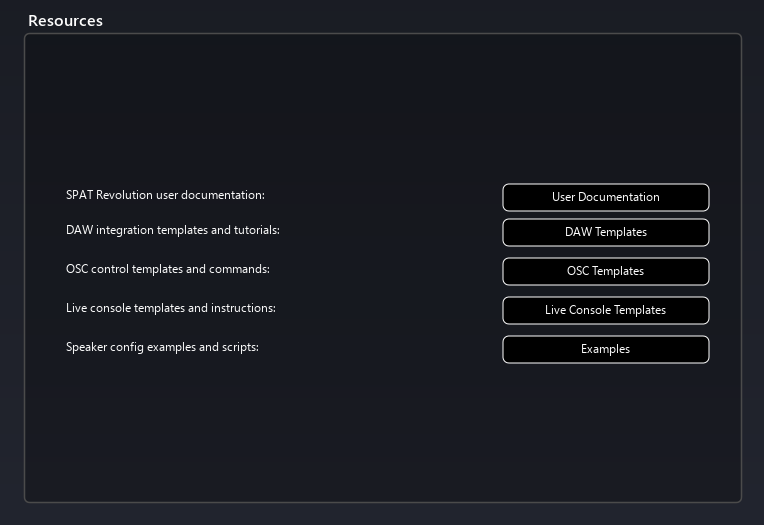
\includegraphics{index_files/mediabag/Resources.png}

This box gives you direct access to many resources related to \emph{SPAT
Revolution}: - This documentation - DAW templates for using LAP: Ableton
Live, Apple Logic Pro X, Avid ProTools, Steinberg Nuendo, Merging
Technologies Pyramix - OSC templates, which include a lemur template and
a QLab example session - Live console templates: S6L, Digico and SSL -
Examples of various scripts

\hypertarget{global-bars}{%
\chapter{Global Bars}\label{global-bars}}

\hypertarget{navigation-bar}{%
\section{Navigation bar}\label{navigation-bar}}


\includegraphics{index_files/mediabag/TopBar.png}

The Navigation bar appears at the top of all views. As well as links to
different editor views and to the preference, it also offers you the
possibility to mute and unmute rooms.

The status and help bars appear at the bottom of all views. It gives
information about the status of audio connections, sample rate, block
size and through latency. Some inline help also appears here when the
mouse moves over elements of the \emph{SPAT Revolution} graphical user
interface. The \emph{Provide feedback} button sends a message directly
to FLUX:: Immersive support which automatically includes your system
information for our support team.

\hypertarget{status-bar}{%
\section{Status bar}\label{status-bar}}


\includegraphics{index_files/mediabag/StatusBar.png}

The status bar help you easily monitor many critical information about
your hardware and your incoming or outgoing audio stream.

\hypertarget{input-stream}{%
\subsection{Input stream}\label{input-stream}}

Allows monitoring the good reception of audio through LAP. + When ``No
connection'' is displayed, this means that no SPAT Send plug-in with LAP
enabled is seen by \emph{SPAT Revolution}. + When a connection is
validated, it should provide a timecode, corresponding to the DAW
transport position. + If the sample rate or block size is unmatched
between \emph{SPAT Revolution} and the DAW used, the ``all in sync''
mention will turn red and count the sync errors.

\hypertarget{hardware-device}{%
\subsection{Hardware device}\label{hardware-device}}

This section helps you monitor your audio hardware and how it interacts
with \emph{SPAT Revolution}.

\begin{itemize}
\tightlist
\item
  You can see the name of your input \& output device.
\item
  The block size and sample rate of \emph{SPAT Revolution}.
\item
  The whole latency of the system. This depends on the block size and on
  the selected audio interfaces. Using different audio interfaces can
  result in a higher latency.
\end{itemize}

\hypertarget{timecode-source}{%
\subsection{Timecode source}\label{timecode-source}}

Here, you can choose which timecode \emph{SPAT Revolution} should look
at.

\begin{itemize}
\tightlist
\item
  By default, it is set to ``Absolute''. It refers to the clock of your
  computer, no matter of the connection with an audio interface or with
  LAP streams.
\item
  ``LAP Send'' looks at the clock provided by SPAT Sends plug-ins.
\item
  ``LAP Return'' looks at the clock provided by SPAT Returns plug-ins.
\item
  ``Audio hardware'' looks at the clock provided by the selected audio
  interfaces.
\end{itemize}

\hypertarget{timecode}{%
\subsection{Timecode}\label{timecode}}

Let you monitor the timecode seen by \emph{SPAT Revolution}. For proper
operation of snapshots and automations, it should be always running.

\hypertarget{clock-source}{%
\subsection{Clock source}\label{clock-source}}

Choose what clock SPAT should follow. + Internal. + Hardware. + Auto :
use hardware if one is connected.

\hypertarget{support}{%
\subsection{Support}\label{support}}

Allows to send feedback to the FLUX:: Immersive support team.

\begin{quote}
With Send/Return plug-ins, if sampling rate and block size between DAW
and \emph{SPAT Revolution} are different, the status bar will be red.
Double-click on this bar to automatically change them into \emph{SPAT
Revolution}.
\end{quote}

\hypertarget{snapshot-bar}{%
\section{Snapshot bar}\label{snapshot-bar}}

\begin{figure}

{\centering \includegraphics{index_files/mediabag/SnapshotToolbar.png}

}

\caption{Snasphot toolbar}

\end{figure}

This toolbar has been designed to help to handle snapshots without
navigating to the snapshots page. Some of the most important snapshot
actions will be found on it: - Recall the Previous snapshot. - The name
of the Current snapshot. Clicking on it will display the snapshot list,
enabling to recall any snapshot of the list. - Recall the Next snapshot.
- Update the current snapshot. - Enable or disable the Relative Recall.
- Propagate values between snapshots.

\emph{This bar can be hided on the snapshot panel of the
\textbf{Preference} page.}

\begin{quote}
More information about snapshot can be found on the
\textbf{\href{Spat_Environment_Snapshot_Page.md}{snapshots page}}.
\end{quote}

\hypertarget{setup-page}{%
\chapter{Setup Page}\label{setup-page}}

This is where you will generally start a project by designing the
signal-flow graph that you will be working with. The \emph{Setup page}
is also where you manage the loading and saving of projects to disk.

\hypertarget{setup-modules}{%
\section{Setup Modules}\label{setup-modules}}

The \emph{Environment Setup} editor is a modular environment. The signal
flow starts from the inputs at the top of the graph and concludes with
the outputs at the bottom. You add modules to rows using the small +
icon to the left of the window. Modules are:

\begin{itemize}
\tightlist
\item
  \href{Spat_Environment_Input_Modules.md}{Inputs}
\item
  \href{Spat_Environment_Input_Transcoder_Modules.md}{Input Transcoders}
\item
  \href{Spat_Environment_Source_Room_Modules.md}{Sources}
\item
  \href{Spat_Environment_Source_Room_Modules.md}{Rooms}
\item
  \href{Spat_Environment_Master_Section_Modules.md}{Sums}
\item
  \href{Spat_Environment_Master_Section_Modules.md}{Master Transcoders}
\item
  \href{Spat_Environment_Master_Section_Modules.md}{Masters}
\item
  \href{Spat_Environment_Master_Section_Modules.md}{Binaural Monitors}
\item
  \href{Spat_Environment_Output_Modules.md}{Outputs}
\end{itemize}

\hypertarget{stream-types-and-associated-options}{%
\section{Stream types and associated
options}\label{stream-types-and-associated-options}}

Modules blocs are characterized by their stream type. In spatial audio,
audio streams can be of different natures, as seen in the
\href{}{Spatialisation Technology} section.

Stream types and their options are : + \textbf{Channel-based} : most
common used bloc where one channel correspond to one speaker or one
microphone. + Speaker arrangment : allow to select the channel
configuration of the bloc. + \textbf{HOA} : generic ambisonic bloc. +
\textbf{Order} : select the ambisonic order from 1 to 7. +
\textbf{Dimension} : select between a 2D or 3D sound scene. +
\textbf{A-Format} : pre-encoding ambisonic stream (raw ambisonic
microphone output). + \textbf{B-Format} : \textbf{deprecated, prefer a
3D HOA first order bloc.} + \textbf{UHJ} : special 3D first order
ambisonic stream meant for archiving and stereo compatibility. +
\textbf{MS} : Mid-side. + \textbf{Binaural} : headphone oriented render
using HRTF. + \textbf{Transaural} : binaural decoding on speaker.

\hypertarget{the-graph-editor}{%
\section{The graph editor}\label{the-graph-editor}}

The modular graph editor handles basic mouse editing.

\hypertarget{module-selection}{%
\subsection{Module selection}\label{module-selection}}

Modules can be select by clicking on them. To select several ones, hold
Ctrl/Cmd while clicking on additional modules. It is also possible to
use a marquee selection by left-clicking, holding the button, and
dragging the mouse over the modules you want to select.

\hypertarget{drag-drop}{%
\subsection{Drag \& Drop}\label{drag-drop}}

The drag and drop feature allows an easy and ergonomic way to connect
and reorganize modules in the setup page.

\textbf{Connect modules}

To create a connection between two modules, simply drag one on the
other. SPAT will automatically connect the two modules. If it is
necessary, SPAT will also create supplementary modules if needed. For
example, if we drag and drop an input on a room, SPAT will automatically
create a ``source'' block between them.

This feature also works on a selection of multiple modules of the same
type. For example, if we wished to connect 5 inputs to 1 output, we can
select our inputs a drag them on the output. All the input modules will
be patched to a room block through sources, and the room is a patch to
the output through a master block, with the default stereo room that can
be changed later.

\textbf{Reorganize modules}

The drag and drop feature also allows reorganizing the modules of the
same type. This means that you can now change the order of already
created modules. This gives to the setup page a more ergonomic and
flexible feel.

!\textgreater{} Important to note that this will be changing the index
number of the source. So be careful with automation already created.
This is specific to OSC like using the plugins with OSC where the index
is important. Not the case with software sources/inputs which use a
different ID system.

\hypertarget{the-setup-wizard}{%
\section{The setup wizard}\label{the-setup-wizard}}

In our effort to make \emph{SPAT Revolution} easier to use, we created a
small utility to help you set up new SPAT sessions. This is used mainly
when dealing with hardware I/O.

To open it, you can either:

\begin{itemize}
\tightlist
\item
  Click on the Setup Wizard button in the top menu of the Setup page;
\item
  Go to the main menu, into setup, then ``Setup Wizard'';
\item
  Or, use ALT + W (the shortcut is not working in Windows).
\end{itemize}

The top part of the setup wizard allows to create a new room (with
associated options) or to select an existing room to patch new sources
into. If a new room is created, we can choose its stream type and many
options linked to it. We can also choose to associate a binaural
monitoring block to it (virtualizing the room output). Lastly, for each
new room created, a master block and an output block is also created.

The main part of the wizard allows creating up to 8 different types of
sources. It works like a table where each line can be used for a
specific input stream type. To add or remove a line, simply click on the
+ or - sign on the left side of a line. You can also use the shortcut
Ctrl/Cmd + Go Down or Ctrl/Cmd + Go Up.

Other shortcuts have been implemented in this wizard: - Go up and Go
down to increase / decrease the number of sources - Go Left or Go Right
to change the Stream Type. - Ctrl/Cmd + Go Left or Ctrl/Cmd + Go Right
to change the format (if Channel Based), or the Dimension (if HOA). -
Ctrl/Cmd + Shift + Go Left or Ctrl/Cmd + Shift + Go Right to change the
Order (if HOA).

When we are done creating out different sources, we have two ways to
validate the operation. We can either click on Ok, all the sources,
rooms and outputs will be created, with a straight routing, or, we can
choose to click on Ok + matrix. This last option will open the input and
output matrix of our whole \emph{SPAT Revolution} session to allow us to
quickly customize or validate our patch. Also, if you need to easily
create a line in SPAT matrix, simply hold Ctrl and click on the starting
point of your line.

\hypertarget{action-menu}{%
\section{Action menu}\label{action-menu}}

This menu handles basic operation of modules, like connecting,
disconnecting and renaming. Some of these actions are contextual, and
depend on the block, or the number of modules selected.

!\textgreater{} Note that there is no undo in \emph{SPAT Revolution}.
Think twice before operating and save regularly.

\hypertarget{remove-selected}{%
\subsection{Remove selected}\label{remove-selected}}

Remove the selected modules.

\hypertarget{duplicated-selected}{%
\subsection{Duplicated selected}\label{duplicated-selected}}

Duplicate the selected modules.

\textbf{Room duplication}

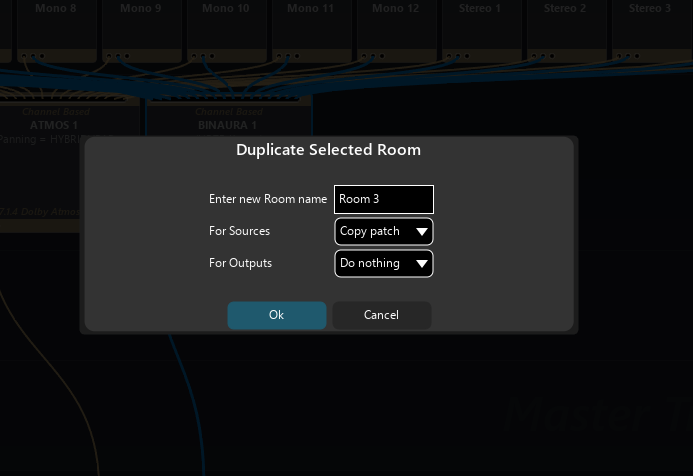
\includegraphics{index_files/mediabag/RoomDuplicate.png}

\emph{SPAT Revolution} allows to quickly duplicate a room with a few
options to help the user to optimize the routing process. To access this
menu, simply click on the Duplicate Selected button, when only a room
selected.

The new pop-up windows allows to: * Rename the duplicated room * Choose
if the sources routed to the original room are routed the new one, or
duplicated, or nothing is patched. * Choose if the outputs of the
original rooms are duplicated, mirrored or nothing is done to the
duplicated room.

\hypertarget{connect-selected}{%
\subsection{Connect selected}\label{connect-selected}}

Connect selected modules. Modules can be connected to multiple
destinations.

\begin{quote}
\emph{SPAT Revolution} will always try to guess what you try to achieve.
For exemple, you can connect an input block directly to an output block
and SPAT will create necessary modules in-between.
\end{quote}

\hypertarget{disconnect-selected}{%
\subsection{Disconnect selected}\label{disconnect-selected}}

Disconnect \textbf{both} inputs and outputs of the selected modules.

\hypertarget{disconnect-selected-inputs}{%
\subsection{Disconnect selected
inputs}\label{disconnect-selected-inputs}}

Disconnect connected inputs of selected modules.

\hypertarget{disconnect-selected-output}{%
\subsection{Disconnect selected
Output}\label{disconnect-selected-output}}

Disconnect connected outputs of selected modules. \#\#\# Disconnect
between selected

Disconnect the connections between selected modules.

\hypertarget{routing-matrix}{%
\section{Routing Matrix}\label{routing-matrix}}

As you can imagine routing and patching high density channel counts can
get complicated. When it comes to that, the SPAT routing matrix is there
to help. You will find it at many points throughout the
\textbf{Environment Setup} graph.

\begin{figure}

{\centering 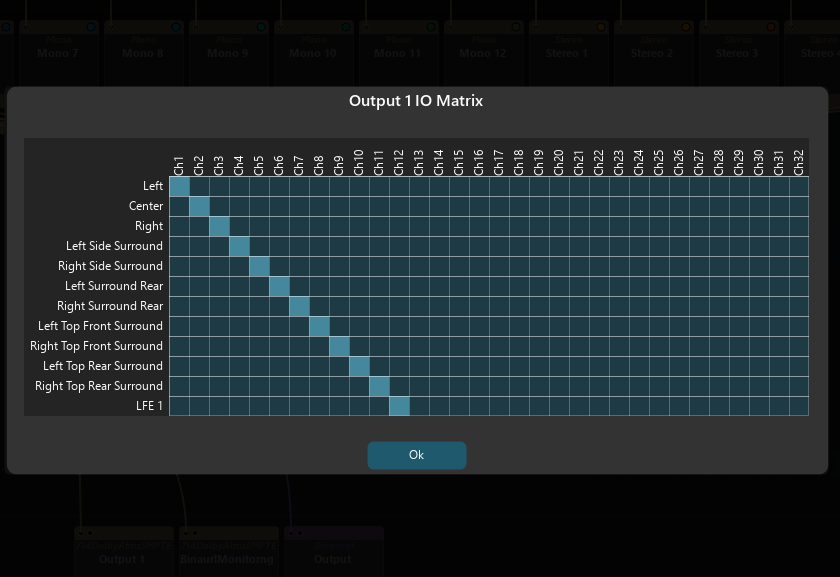
\includegraphics{index_files/mediabag/OutputMatrix.png}

}

\caption{width=800, atl=\emph{SPAT Revolution} Matrix}

\end{figure}

\begin{quote}
\emph{Avoid cable swapping on the loudspeaker setup, use software
routing instead.}
\end{quote}

The routing matrix is available on hardware input and output for routing
as well as for remapping within some modules input and output: Input
transcoder, Master, and Master transcoder.

The speaker configuration editor, a clear channel labeling and the
built-in routing matrix system all help to make the process of signal
routing, checking and debugging more straightforward on location, in the
virtual mix and in the studio.

\begin{quote}
The shortcut Ctrl + click will route one per one all the following
channels.
\end{quote}

Master transcoder and master matrix support summing, thus, one input can
be connected to several outputs, or the opposite.

\hypertarget{inputs-module}{%
\chapter{Inputs Module}\label{inputs-module}}


\includegraphics{index_files/mediabag/InputModuleRow.png}

\emph{SPAT Revolution} itself does not play audio files. The input blocs
are here to access to audio streams and process them in the \emph{SPAT
Revolution} spatialization engine. Input blocs are represented at the
top row of the signal graph.

There are two types of input blocs: + Hardware blocs, which look at
signal coming from an actual audio interface, + Software blocs, which
are tied to a SPAT Send plug-in instances in a DAW.

To create a hardware blocs, click one of the \emph{+} button at the left
of the row. To create a software bloc, instantiate a SPAT Send plug-in
in a DAW and activate its local audio path. You will find more
information on local audio path in the
\href{Ecosystem_\&_integration_DAW_Automation_Local_Audio_Path.md}{8.5
Plug-ins: Local audio path} section.

\hypertarget{name}{%
\section{Name}\label{name}}

Allows to edit the name of an input. It is possible to edit several
names at once by selection several blocs and clicking on the ``Input
Name Wizard'' button in the inspector.

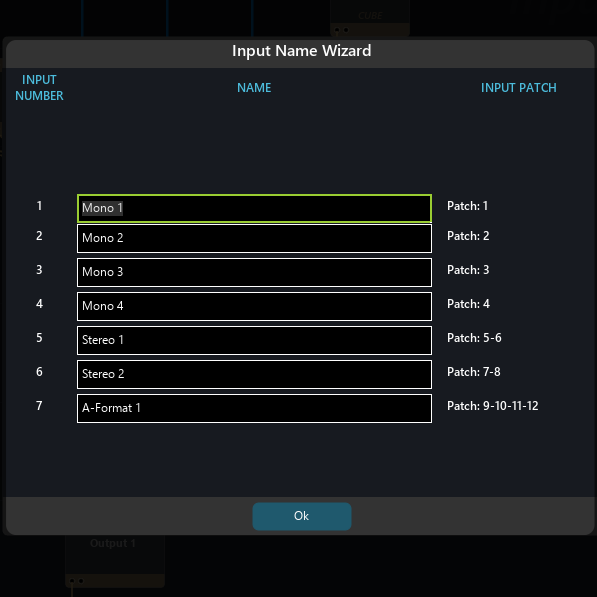
\includegraphics{index_files/mediabag/InputNameWizard.png}

\hypertarget{inputs-configuration}{%
\section{Inputs configuration}\label{inputs-configuration}}

\begin{itemize}
\tightlist
\item
  Input type : allow to select if the source of the signal is coming
  from the selected input or from the signal generator included in
  \emph{SPAT Revolution}. The nature of the generated signal can be
  changed in the \href{Application_Preferences.md}{Preference page}.
\item
  Input stream : allow to select the stream type of the bloc.
\end{itemize}

\begin{quote}
Input stream types are : channel-based, HOA, A-Format, B-Format, UHJ,
MS, Binaural and Transaural.
\end{quote}

For more options related to stream type, check the
\href{Spat_Environment_Setup_Page.md}{Setup Page} section.

\hypertarget{routing}{%
\section{Routing}\label{routing}}

Give access to the routing matrix

!\textgreater{} This option is only available on hardware input.

\hypertarget{levels}{%
\section{Levels}\label{levels}}

Basic true peak metering for each block's channels.

\hypertarget{delay}{%
\section{Delay}\label{delay}}

Each input comes with a delay which can be useful: - in live situation,
to compensate delay between microphones. - in studio situation, to
compensate the plugins delay when using Local Audio Path.

The delay can be set in samples, milliseconds, or distance unit (meters
if metric system, feet otherwise). This can be chosen on the
\textbf{Global} panel of the \textbf{Preferences} page.

\hypertarget{input-transcoder}{%
\chapter{Input Transcoder}\label{input-transcoder}}

\emph{SPAT Revolution} can handle many formats of multichannel audio
throughout the signal flow, as we have been pointing out. As we approach
the actual virtualisation of inputs into object-based audio sources in
the SPAT \emph{Virtual Rooms} it may be necessary to change from the
original input format to another. You use the Input Transcoder module
and its parameters to do this.

\includegraphics{index_files/mediabag/InputTranscoding.png}

The transcoder modules may modify the channel count of the stream
passing through it, depending on the format transfer being requested.
For example, transcoding from Ambisonic B-Format into a Channel Based 3D
Cube involves a four-channel Ambisonics stream getting transcoded into
an eight-channel stream grouped and treated as a specific speaker
configuration.

\hypertarget{transcoding-matrix}{%
\section{Transcoding Matrix}\label{transcoding-matrix}}

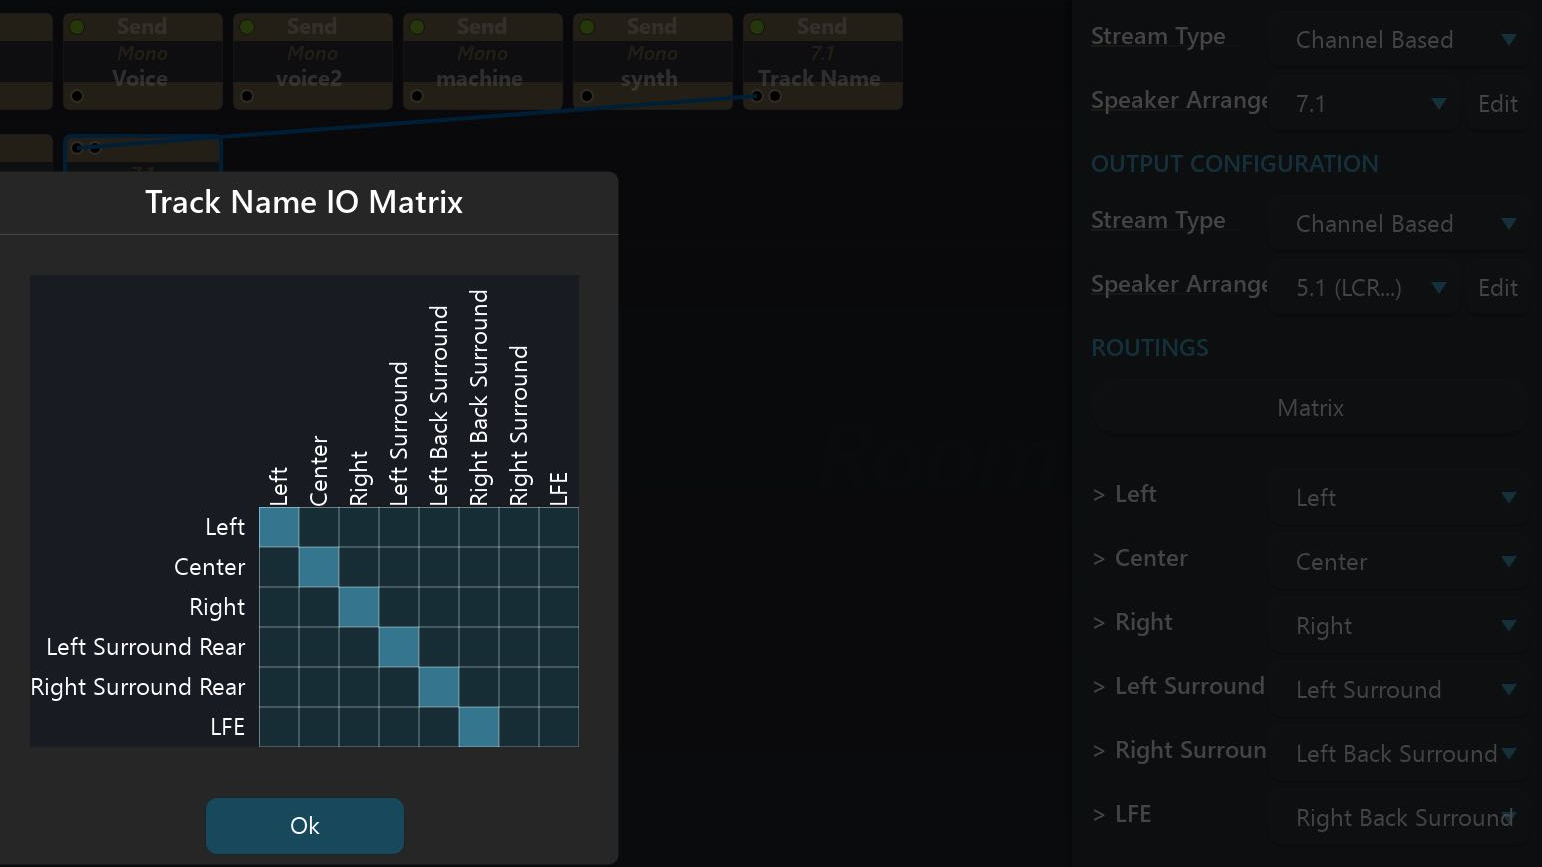
\includegraphics{index_files/mediabag/TranscoderMatrix.png}

In the case where an incoming Channel Based stream needs transcoding
into an outgoing Channel Based stream which has fewer channels, the IO
Matrix is used to remap the output format by dropping some input
channels. This is not strictly \emph{Transcoding} or \emph{decoding} but
is a useful tool to have in a certain format changing scenarios. This
matrix does not give the possibility to up-mix or down mix. To properly
up mix or down mix, it is advisable to use a room to take the virtual
source of one format, and output with the desired end format.

\hypertarget{when-to-transcode-inputs}{%
\section{When to Transcode Inputs?}\label{when-to-transcode-inputs}}

The main reason you will need to transcode inputs is when you are mixing
and spatializing inputs in a \emph{SPAT Revolution} \emph{Virtual Room}.
This is because the \emph{Virtual Room} module requires incoming sources
to be in a Channel Based format. Internally, the Room may well be
panning in Channel based, Ambisonics or binaural format, but it always
needs Channel Based streams as inputs. More about this in the
\emph{Virtual Room} section. Format transcoding may not always need
re-spatializing in a room. There are some contexts where you will not
use a Virtual Room in the signal flow,

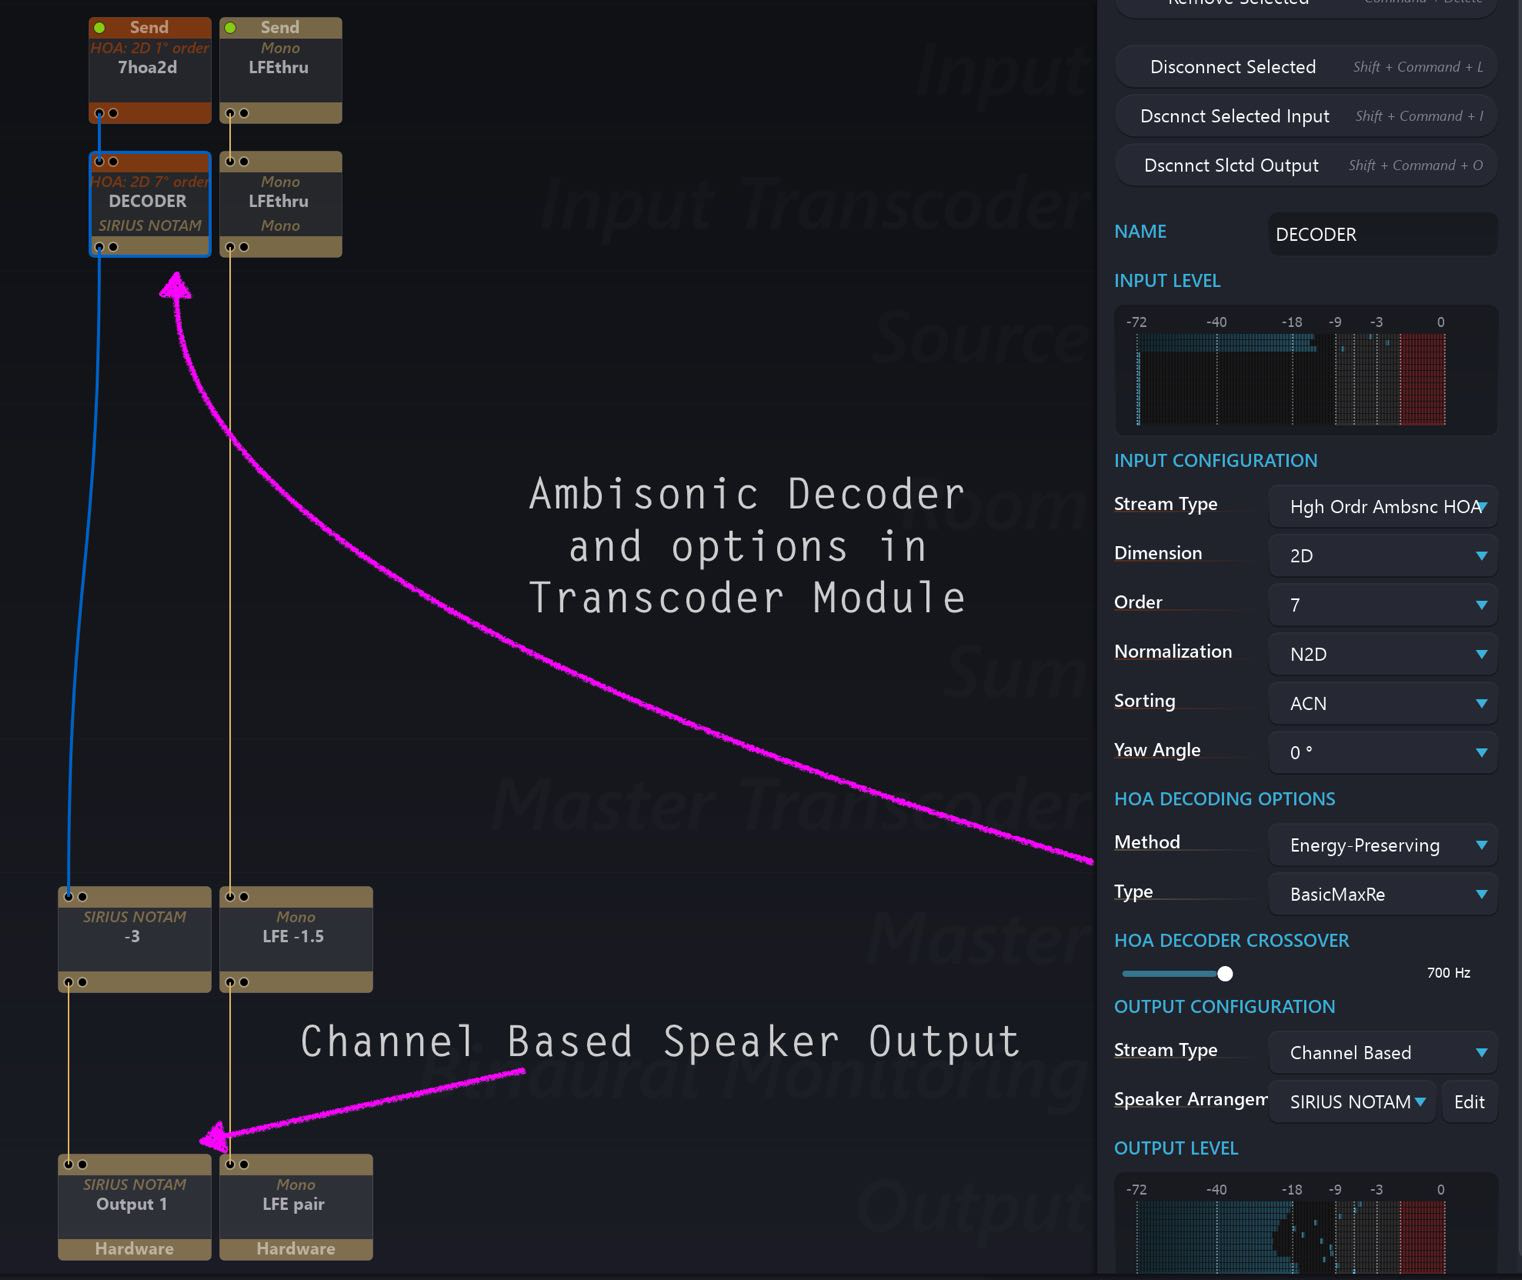
\includegraphics{index_files/mediabag/TranscodingExplained.png}

Here is an example of decoding an ambisonic signal using an input
transcoder module. This could also be done in the master transcoder
section of the graph.

As mentioned in
\href{Spatialisation_Technology_Scene_based_streams.md?id=introduction-to-ambisonics}{Introduction
to Ambisonics}, a decoding stage is absolutely necessary to render
Ambisonics encoded audio to speakers. It can be done like this without
the need of a room.

\hypertarget{aggregation-of-input}{%
\section{Aggregation of input}\label{aggregation-of-input}}

As some DAW does not support multichannel tracks, \emph{SPAT Revolution}
provides on the input transcoder a way to aggregate stereo or mono input
in order to make multichannel sources.

To do it, connect several inputs on the same input transcoder or source
and select on it the wanted format. When selecting it, a combobox
``Aggregate Input'' will appear, and will allow to aggregate all the
inputs.

\begin{figure}

{\centering \includegraphics{index_files/mediabag/InputAggregation.png}

}

\caption{Input aggregation}

\end{figure}

!\textgreater{} The order of the channel is determined by the connection
order to the input transcoder or source.

\hypertarget{sources-rooms-module}{%
\chapter{Sources \& Rooms Module}\label{sources-rooms-module}}

\hypertarget{source-module}{%
\section{Source module}\label{source-module}}

Sources' modules are very important and quite unique ones. This is where
the object-oriented mixing of SPAT Revolution takes in.

Sources' modules associated metadata to incoming audio streams. Because
of their object-oriented nature, \textbf{they can only input and output
channel-based streams}. In practice, this means you cannot patch, for
example, an ambisonic stream to a room, even if the room in question is
ambisonic itself. It first needs to be transcoded by using and input
transcoder.

The so-called metadata is the source parameters, such as position and
reverberation information. All these parameters are explained in the
section \href{Spat_Environment_Source.md}{Source properties}.

One source can be connected to several rooms. This is one of the
advantages of the object-based mixing: it allows to create different
mixes in different formats with the same exact information.

\hypertarget{name-1}{%
\subsection{Name}\label{name-1}}

Allows renaming a source. By default, it takes the name of the input
patched into it.

\hypertarget{io-configuration}{%
\subsection{IO Configuration}\label{io-configuration}}

Allows selecting the speaker arrangement used by the source. It can be
selected from the list or user defined.

Multi-channel sources is one of the unique SPAT Revolution features.

\begin{quote}
If you struggle to understand why we talk about speakers at this stage,
simply consider them as ``virtual'' speaker that will be emitting in a
``virtual'' room.
\end{quote}

!\textgreater{} A source can and should only be channel-based!

\hypertarget{tracking}{%
\subsection{Tracking}\label{tracking}}

SPAT Revolution is able to receive data from RTTrPM open protocol
tracking systems. This protocol is supported by BlackTrax™. BlackTrax™
is a vision-based system that connects to different third-party
applications, such as robotic lights, media servers and SPAT Revolution.
OSC is the other very good method to use for tracking, and various
tracking systems support it natively.

!\textgreater{} \emph{RTTrPM protocol is not available with the
\textbf{Essential} license of SPAT Revolution}.

When you have correctly set up the BlackTrax protocol (see
\href{ThirdParty_BlackTrax.md}{BlackTrax Integration section}) then you
can directly assign Tracking Number to virtual sources, and also to
listener position (see
\href{Spatialisation_Technology_Listener_Position.md}{Listener position
section}) for advanced virtual reality interactive audio projects.

\hypertarget{gain}{%
\subsection{Gain}\label{gain}}

Change the input gain of the source.

\hypertarget{levels-1}{%
\subsection{Levels}\label{levels-1}}

Basic true peak metering for each block's channels.

\hypertarget{room-module}{%
\section{Room module}\label{room-module}}

If sources are where localization information is stored, rooms are where
the ``interpreting'' happens. A room is defined by two main criteria:
its output stream type and its reverberation. Simply, a room module look
at all the information stored in sources and then act as a renderer for
a given format.

It is a classic case of object-based mixing, where source modules
associate metadata to channels, and room modules interpret them.

!\textgreater{} Only source modules can be connected to room modules.

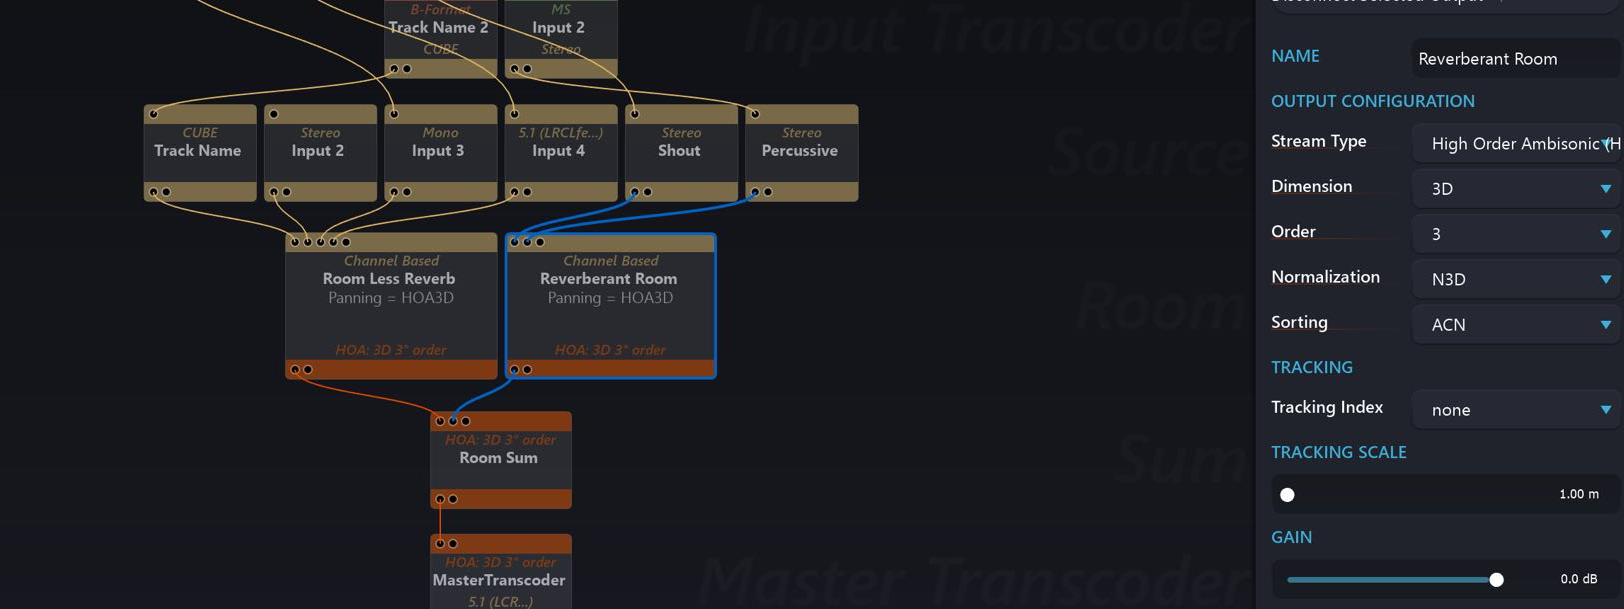
\includegraphics{index_files/mediabag/SessionWithRoomSelected.png}

The first thing to notice is that we can add any number of rooms. In the
screenshot above, two HOA 3D rooms are being used, each with differently
designed acoustics. SPAT revolution offers flexibility, in order to
encompass different workflow ideas or experimental approaches. For
example, the same virtual sources may be assigned into multiple rooms,
with multiple end destinations. Or as in the screenshot above, virtual
sources might exist in different spaces that get summed together.

!\textgreater{} The \textbf{Essential} license limits the number of
active (processed) rooms to one (1). The other are deactivated (not
processed).

\hypertarget{name-2}{%
\subsection{Name}\label{name-2}}

Allow renaming a room.

!\textgreater{} Rooms cannot share the same name!

\hypertarget{io-configuration-1}{%
\subsection{IO Configuration}\label{io-configuration-1}}

Allow selecting the rendering type and the associated options.

\textbf{Stream Type} :

\begin{itemize}
\tightlist
\item
  Channel Based
\item
  HOA
\item
  Binaural
\item
  MS
\item
  B-Format (depreciated, please use HOA 1st order room connected to a
  master transcoder to transform it on B-Format standard)
\end{itemize}

\hypertarget{tracking-1}{%
\subsection{Tracking}\label{tracking-1}}

See \href{Spatialisation_Technology_Listener_Position.md}{Listener
position section}.

\hypertarget{gain-1}{%
\subsection{Gain}\label{gain-1}}

Change the output level of the room.

\hypertarget{levels-2}{%
\subsection{Levels}\label{levels-2}}

Basic true peak metering for each block's channels.

\hypertarget{master-section}{%
\chapter{Master Section}\label{master-section}}

The \textbf{Sum} row of modules is used to mix the output of two or more
rooms of the same output configuration and in some contexts, to sum
inputs directly without the use of room.

The \textbf{Sum} module can handle different input configurations. It
will Sum channels based on their channel names, so a correct naming
convention is important. Summing a 5.1 and 7.1 rooms together will
output a 7.1 where their common L, C, R, Left and Right Surround rear
channels will have content summed from both rooms the but Left and Right
Back surround will be only from the 7.1 room.

\begin{quote}
Summing can also be done directly in \textbf{Master} and \textbf{Output}
Modules, but summing into a \textbf{Sum} module will save resources if
the same sum is performed in different blocks.
\end{quote}

The \textbf{Master Transcoder} row of modules offers an opportunity to
consolidate the various formats you might have been mixing into one (or
more) formats for final output routing by the \textbf{Output} modules.
The same options and routing are available as in the
\href{Spat_Environment_Input_Transcoder_Modules.md}{Input Transcoder
modules}.

The \textbf{Master} bloc gives you a last gain staging control, as well
as down mixing capabilities. When opening its matrix, it is possible to
patch several inputs to one output, or, one input to several outputs.

\begin{figure}

{\centering \includegraphics{index_files/mediabag/MasterMatrix.png}

}

\caption{Master matrix}

\end{figure}

Finally, the
\href{5_Spatialisation_Technology_5_1_Binaural_5_1_Binaural?id=binaural-monitoring-module.md}{\textbf{Binaural
Monitoring}} row provides a way to decode the whole scene to headphones
only in binaural 3D.

\hypertarget{output}{%
\chapter{Output}\label{output}}

The main thing to note at the output stage is that you can have any
number of output routes. Like the
\href{6_Spat_Environment_6_4_Inputs_6_4_Inputs.md}{Inputs}, they may be
either direct hardware routes, which returns audio streams (via matrix
routing) to the physical outputs of an audio interface connected to your
\emph{SPAT Revolution} workstation. The Hardware Output workflow is the
most direct way to render in realtime to an actual loudspeaker system
(or headphones).

!\textgreater{} Software outputs are created by the instantiation of a
SPAT Return plug-in in a compatible DAW, when its local audio path is
set to ``on''.

Outputs may also be linked to \emph{SPAT Revolution} RETURN plug-ins,
which returns audio streams internally on the same workstation to a
valid SPAT RETURN plug hosted in your DAW. The software RETURN workflow
offers an easy way to render the spatial scene to disk, as
\emph{Ambisonic encoded}, \emph{Binaural encoded} or \emph{Sound system
encoded} multichannel audio.

\begin{quote}
Create multiple output routes to capture Ambisonic recordings at the
same time as sound system specific rendering.
\end{quote}

\includegraphics{index_files/mediabag/OutputSelected.png}

\hypertarget{modules-channel-count}{%
\chapter{Modules Channel Count}\label{modules-channel-count}}

Into \emph{SPAT Revolution}, modules are treated exactly the same
whether there are mono or multichannel, ambisonics, binaural or
channel-based.

\hypertarget{mono-input}{%
\section{Mono Input}\label{mono-input}}

A one channel audio stream is always treated as a mono signal. It will
appear in a \emph{Virtual Room} as one positionable virtual source with
its own directivity and parameters. In many ways, mono signals are the
most straightforward format to work with in a spatial composition. This
is because a one channel signal discretely contains all its acoustic and
spectral properties without inter-channel dependencies, such as those
found in a wide stereo image, for example. In practice, such point
sources are easier to localise and balance spatially with others.

\begin{quote}
Mono sources are simple to work with when balancing a spatial mix.
\end{quote}

\hypertarget{two-channel}{%
\section{Two Channel}\label{two-channel}}

A two-channel audio stream will appear in the \emph{Virtual Room} as two
mono sources linked together as a group. A two-channel audio input will
already open a few more choices for disambiguating the configuration.
SPAT needs to know what format the two channels are in, so it knows how
to correctly handle the audio stream later in the signal flow.

\begin{itemize}
\tightlist
\item
  \textbf{Channel Based} Treated as Normal stereo
\item
  \textbf{Mid-Side (MS)} Treated as Mid Side encoded stereo
\item
  \textbf{Binaural / Transaural} Treated as encoded 3D stereo
\end{itemize}

\hypertarget{four-channel-input}{%
\section{Four Channel Input}\label{four-channel-input}}

The next significant channel count that needs disambiguation from the
user is a four-channel stream.

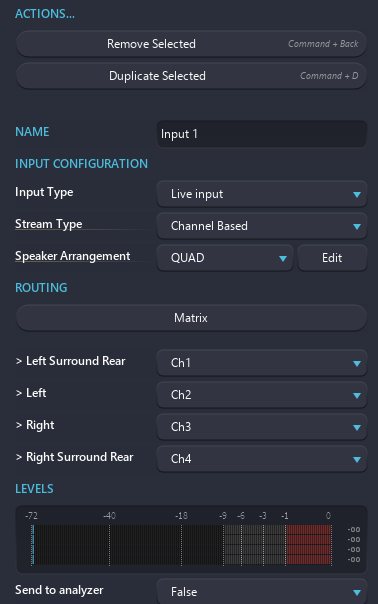
\includegraphics{index_files/mediabag/InputInspectorQuad.png}

A four-channel stream could contain the format of a four-speaker Channel
Based formats (QUAD, 4.0, LCRS) but could also contain different formats
of interleaved four-channel Ambisonic audio (A-Format, B-Format). You
can read more about A-Format and B-Format in the
\href{Scene_based_streams.md}{Ambisonics} section of this user guide.
The important thing to remember here is that confusing Ambisonic audio
and Channel Based audio is a significant mistake, even though you might
hear something `wide sounding.'

!\textgreater{} Do not confuse multi-channel-based audio formats with
multichannel Ambisonic audio formats. They may have the same channel
counts but are completely different!

\hypertarget{multi-channel-based-input}{%
\section{Multi-Channel Based Input}\label{multi-channel-based-input}}

Any input module configured to represent a stream of multichannel audio
can be configured as a Speaker Arrangement format which would require
that number of channels, as a minimum. For example, \emph{DTU 7.1} needs
8 channels, and \emph{DTU 5.1} needs 6. \emph{Auro3D 13.1} needs 14
channels. Unfortunately, things can get complicated in practice, as
there are a few variations of standardised speaker layouts which have
the same number of channels and seem very similar - but need
disambiguation. This is important to get right, and will depend a lot on
the context of your project and on changing standards in the audio
industry. For example, at least four different 7.1 routing standards are
to be found `in the wild' and it's important to know which one you are
actually dealing with. Often, for example, the so-called low-frequency
effects channel in cinema surround formats, is not always on the same
channel.

!\textgreater{} \textbf{Essential} license of \emph{SPAT Revolution}
limits total number of channels to 32 input channels and to 18 output
channels.

\begin{quote}
Try to stick to industry standard channel naming conventions throughout
a cinematic surround sound project.
\end{quote}

\begin{longtable}[]{@{}lll@{}}
\toprule()
L & C & R \\
\midrule()
\endhead
sL & & sR \\
surround Left & & surround Right \\
LFE & & \\
Low Frequency Effects & & \\
sbL & & sbR \\
surround back Left & & surround back Right \\
\bottomrule()
\end{longtable}

\begin{quote}
\begin{itemize}
\tightlist
\item
  Some common Speaker Channel naming abbreviations.
\end{itemize}
\end{quote}

\hypertarget{session-compatibility-and-modules-deactivation}{%
\chapter{Session compatibility and modules
(de)activation}\label{session-compatibility-and-modules-deactivation}}

\emph{SPAT Revolution} Essential version aims at being a limited version
of Ultimate one. Then, it has the same workflow but limited capacities.

\hypertarget{create-and-edit-a-session-in-essential-version}{%
\section{Create and edit a session in Essential
version}\label{create-and-edit-a-session-in-essential-version}}

Any type of session can be created and edited with \emph{SPAT
Revolution} Essential version. This includes the opening and editing of
Ultimate sessions with Essential version. However, due to license
restrictions, the blocks that do not fit the restrictions are
automatically deactivated, and thus not processed. If the block
deactivation is due to a license restriction, the deactivation reason
appears in the block's configuration panel on the \textbf{Setup} page:

\includegraphics{index_files/mediabag/RoomDeactivation.png}

It is possible to manually activate/deactivate blocks on the block
inspector of the \textbf{Setup page}:

\includegraphics{index_files/mediabag/DeactivatingBlock.png}

Evidently, if a block has been deactivated for license limitations
reasons, the block cannot be manually activated.

\hypertarget{opening-an-ultimate-session-with-essential-version}{%
\section{Opening an Ultimate session with Essential
version}\label{opening-an-ultimate-session-with-essential-version}}

If a session contains non-authorized objects or configurations, the
concerned blocks are deactivated and the session behavior is the same as
described in the ``Create and edit a session in SPAT Essential'' section
above.

\hypertarget{opening-an-essential-session-with-ultimate-version}{%
\section{Opening an Essential session with Ultimate
version}\label{opening-an-essential-session-with-ultimate-version}}

If a session contains inactive blocks that could be activated, a dialog
offers to activate them:

\includegraphics{index_files/mediabag/BlocksActivation.png}

\hypertarget{check-essential-compatibility-in-spat-revolution-ultimate}{%
\section{Check Essential compatibility in SPAT Revolution
Ultimate}\label{check-essential-compatibility-in-spat-revolution-ultimate}}

In the Menu File, click on the Check Essential Compatibility item to
check if the current session is compatible with the Essential version
restrictions. A dialog then informs of the compatibility.

\includegraphics{index_files/mediabag/EssentialCompatible.png}
\includegraphics{index_files/mediabag/EssentialNotCompatible.png}

If the session is not compatible, it can be opened in Essential version
but the non-authorized objects will be automatically deactivate (see
paragraph ``Create and edit a session in \emph{SPAT Revolution}
Essential'' above).

\begin{quote}
The blocks contained in an Ultimate session can be manually deactivated
to fit the Essential version restrictions. The check for compatibility
answers that the session is compatible.
\end{quote}

\hypertarget{essential-compatibility-mode-for-ultimate-version}{%
\section{Essential Compatibility Mode for Ultimate
version}\label{essential-compatibility-mode-for-ultimate-version}}

When in Ultimate version, a Compatibility Mode allows it to behave as an
Essential version (see paragraph ``Create and edit a session in SPAT
Essential'' above).
\includegraphics{index_files/mediabag/EssentialCompatibilityModeOn.png}

If the current session is compatible with Essential version a dialog
informs the user:

\includegraphics{index_files/mediabag/EssentialAlreadyCompatible.png}

\hypertarget{items-page}{%
\chapter{Items' page}\label{items-page}}

This page gives an overview and allows to edit the major parameters for
each item type (Input, Source, Room, etc.)

\begin{figure}

{\centering \includegraphics{index_files/mediabag/Page11.png}

}

\caption{The items' page}

\end{figure}

The following video illustrates some possibilities that this page
offers.

\hypertarget{items-type-selection}{%
\section{Items type selection}\label{items-type-selection}}

The upper left list control allows to choose which kind of items you
want to display in the Items' Page.

\hypertarget{parameters}{%
\section{Parameters}\label{parameters}}

Depending on the selected item's type, the editable parameters are the
following.

\hypertarget{common-parameters}{%
\subsection{Common parameters}\label{common-parameters}}

For all items, the items' page allows quick edition of:

\begin{itemize}
\tightlist
\item
  \textbf{Number}: the item number order of the list.
\item
  \textbf{Name}: edit this field to change the name of the item.
\item
  \textbf{Active}: define if the item is computed or not. \emph{If the
  item is inactive due to license restriction, the field cannot be
  edited.}
\end{itemize}

\hypertarget{input-specific-parameters}{%
\subsection{Input specific parameters}\label{input-specific-parameters}}

In addition to the common parameters, when the \emph{Input} item's type
is selected, the Items' Page shows:

\begin{itemize}
\tightlist
\item
  \textbf{Type}: displays if the input is \emph{Live input} or
  \emph{Signal generator}.
\item
  \textbf{Speaker arrangement}: select the speaker arrangement of the
  input.
\item
  \textbf{Delay (smp)}: define the input delay in sample.
\item
  \textbf{Delay (ms)}: define the input delay in ms.
\item
  \textbf{Delay (meters)}: define the input delay in meters.
\item
  \textbf{Delay (feets)}: define the input delay in feets.
\item
  \textbf{Connected}: displays if the input is connected to other items.
\end{itemize}

\begin{figure}

{\centering \includegraphics{index_files/mediabag/Inputs.png}

}

\caption{Items page for sources}

\end{figure}

\hypertarget{source-specific-parameters}{%
\subsection{Source specific
parameters}\label{source-specific-parameters}}

In addition to the common parameters, when the \emph{Source} item's type
is selected, the Items' Page allows quick edit of:

\begin{itemize}
\tightlist
\item
  \textbf{Color}: select the color of the source.
\item
  \textbf{Room}: list the rooms' names the source belongs to. \emph{The
  rows can be grouped by rooms. See
  \protect\hyperlink{Groupux5cux2520sourcesux5cux2520byux5cux2520rooms}{Group
  sources by rooms}}
\item
  \textbf{Speaker arrangement}: select the speaker arrangement of the
  source.
\item
  \textbf{Remote}: define if the source can be controlled by OSC or not.
\item
  \textbf{Remote number}: define the index of the source on OSC side.
  \emph{If set to 0, the remote number is equal to the source number.
  Careful with this behavior: this will be edited with the source
  order.}
\item
  \textbf{Automation}: define if the source can be controlled by
  automation via Local Audio Path.
\item
  \textbf{Snapshot}: define if the source can be controlled by snapshot
  recall.
\item
  \textbf{RTTrPM number}: define the RTTrPM beacon number used for
  control this source. If set to 0, the tracking will be disabled.
  \emph{Ultimate license only.}
\item
  \textbf{Gain}: define the gain of the source.
\item
  \textbf{Mute}: define the mute status of the source.
\end{itemize}

\begin{figure}

{\centering \includegraphics{index_files/mediabag/Sources.png}

}

\caption{Items page for sources}

\end{figure}

\hypertarget{room-specific-parameters}{%
\subsection{Room specific parameters}\label{room-specific-parameters}}

In addition to the common parameters, when the \emph{Room} item's type
is selected, the Items' Page shows:

\begin{itemize}
\tightlist
\item
  \textbf{Connected sources}: displays the number of connected sources.
\item
  \textbf{Speaker arrangement}: select the speaker arrangement of the
  room. For HOA and Binaural room, this field displays respectively the
  dimension and the HRTF.
\item
  \textbf{Pan law}: select the pan law of the \emph{Room}, if stream
  type is Channel-Based or Binaural. For HOA room, this field displays
  the HOA order.
\item
  \textbf{Reverb enable}: define if the reverb is enabled in this room.
\item
  \textbf{Protection zone width}: define the width of the
  \href{/Spat_Environment_Understanding_the_3D_View?id=the-protection-zone}{protection
  zone}.
\item
  \textbf{Efficiency zone}: select the wanted behavior when a source is
  out of the
  \href{/Spat_Environment_Understanding_the_3D_View?id=the-efficiency-zone}{efficiency
  zone} of the room.
\item
  \textbf{Scaling distance}: define the {[}scaling distance{]} of the
  room in meters.
\item
  \textbf{Tracking scaling}: define the tracking scaling of the room in
  meters.
\end{itemize}

\begin{figure}

{\centering \includegraphics{index_files/mediabag/Rooms.png}

}

\caption{Items page for rooms}

\end{figure}

\hypertarget{navigation}{%
\section{Navigation}\label{navigation}}

In order to give an easy navigation on this page and its parameters,
keyboard shortcuts have been implemented, including powerful
multi-selection and edition.

\begin{itemize}
\tightlist
\item
  Up: select the cell of the previous row.
\item
  Shift + Up: add the previous row to the row selection.
\item
  Down: select the celle of the next row.
\item
  Shift + Down: add the next row to the row selection.
\item
  Shift + click: select all the rows in between the two selected
\item
  Ctrl + click: select only the wanted rows.
\item
  Left key: select the previous cell.
\item
  Right key: select the next cell.
\item
  Space on an on/off button: it will toggle the button for the actual
  selection.
\item
  Enter (return) on a string or float edit, or a list: it will begin the
  edit of the selected cell. Using it a second time will edit the cell
  of the next row.
\item
  Home: go to the first row.
\item
  End: go to the last row.
\item
  Page Up: select the cell on the previous page.
\item
  Page Down: select the cell on the next page.
\end{itemize}

It is also possible to sort the items according to a specific field,
shift-clicking on the header of it.

\hypertarget{filtering-and-group-by}{%
\section{Filtering and Group by}\label{filtering-and-group-by}}

To go further in easing the edition of parameters, the Items' page
allows to filter of the displayed data. Moreover, for sources, they can
be grouped according to the rooms they belong to.

\hypertarget{filtering}{%
\subsection{Filtering}\label{filtering}}

Enter text in the top search field to filter the displayed objects. This
will search on all the field. To search for a specific field, type the
name of the field and add ``:''. For example, to search the object with
the name beginning by ``Violin'', type name:Violin.

\hypertarget{group-sources-by-rooms}{%
\subsection{Group sources by rooms}\label{group-sources-by-rooms}}

\hypertarget{snapshots-page}{%
\chapter{Snapshots page}\label{snapshots-page}}

\begin{figure}

{\centering \includegraphics{index_files/mediabag/Page111.png}

}

\caption{Snapshots page}

\end{figure}

The new Snapshots page of \emph{SPAT Revolution} allows the user to
deeply manage its show. Snapshots are an easy way to create different
session states. A classic example would be to have different snapshots
for different songs, or sections of a song, in a live show.

The system built in \emph{SPAT Revolution} is both simple and powerful.
As a generality, when a snapshot is created, it stores the mix
parameters, i.e.~the source, room and master parameters. All parameters
are always stored, but it is possible to filter the recalled parameters.

The page is divided into three different sections: the snapshot list,
the versions' history and the inspector.

\hypertarget{the-snapshot-list}{%
\section{The snapshot list}\label{the-snapshot-list}}

\hypertarget{generality}{%
\subsection{Generality}\label{generality}}

\begin{figure}

{\centering \includegraphics{index_files/mediabag/SnapshotsList.png}

}

\caption{Snapshot list}

\end{figure}

The snapshot list is the main section of snapshot management and serves
many purposes. First, it displays the snapshot organization of your
session. The snapshot name can also be edited by clicking on the text
field. To recall a snapshot from the snapshot list, simply double-click
on the number of one of them.

\hypertarget{snapshot-selection}{%
\subsubsection{Snapshot selection}\label{snapshot-selection}}

A snapshot can have different states. First, it can be selected or
unselected inside the list. It will serve to make a specific action on
the selected snapshot(s) and reveals the versions' history and inspector
section (if only one is selected). The state of selection is a graphical
element that let the user know on which snapshot an action is performed.

\includegraphics{index_files/mediabag/UnselectedSnapshot.png} Unselected
snapshot

\includegraphics{index_files/mediabag/SelectedSnapshot.png} Selected
snapshot

\hypertarget{snapshot-activation-and-deactivation}{%
\subsubsection{Snapshot activation and
deactivation}\label{snapshot-activation-and-deactivation}}

A snapshot can also be disabled using the dedicated toggle. A disabled
snapshot will be darkened in the list. It cannot be recalled. The next
and previous snapshot buttons on the snapshot toolbar will automatically
skip a disabled snapshot.

\includegraphics{index_files/mediabag/SnapshotEnableDisable.png}
Activated snapshot (1) VS. deactivated snapshot (2)

\hypertarget{current-snapshot}{%
\subsubsection{Current snapshot}\label{current-snapshot}}

Lastly, the last recalled snapshot is displayed with the ``current''
field set on. This allows the user to monitor where he is in his show.

\includegraphics{index_files/mediabag/SnapshotRecalled.png} In-play
snapshot (2) VS. not-in-play snapshot (1)

\hypertarget{the-actions}{%
\subsection{The actions}\label{the-actions}}

\begin{figure}

{\centering \includegraphics{index_files/mediabag/SnapshotsListActions.png}

}

\caption{Action bar}

\end{figure}

This snapshot list's top bar regroups all the snapshot actions:

\begin{itemize}
\tightlist
\item
  New allows creating a new snapshot, storing the current sources, rooms
  and masters state.
\item
  Duplicate allows duplicating the current snapshot selected in the
  snapshot list.
\item
  Update allows updating the selected snapshot in the snapshot list with
  the current state of the session. It will create a new snapshot
  version.
\item
  Remove allows deleting the snapshot(s) selected in the snapshot list.
\item
  Move up moves the selected snapshot(s) up one row in the snapshot
  list.
\item
  Move down moves the selected snapshot(s) down one row in the snapshot
  list.
\item
  Recall allows loading a previously saved snapshot selected in the
  snapshot list.
\end{itemize}

!\textgreater{} Keep in mind that source with ``Snapshot'' parameter set
off will be stored, but not recalled. Please check the ``item page''
section for more information.

\hypertarget{snapshot-index}{%
\subsection{Snapshot Index}\label{snapshot-index}}

To recall through OSC a snapshot, the name or the index is required. As
snapshot order can be changed, the snapshot index does not depend on the
snapshot position in the list. The snapshot index is indicated on each
snapshot, on the left side of the recall options.

\begin{figure}

{\centering \includegraphics{index_files/mediabag/SelectedSnapshot.png}

}

\caption{Snapshot index}

\end{figure}

It is possible to generate new indexes for all the snapshots according
to list order. To do so, click on the menu Snapshot/Reindex all
snapshots.

\hypertarget{recall-options}{%
\subsection{Recall options}\label{recall-options}}

Recalling a snapshot will use four different options: - The
\textbf{timing} is the transition time between the current session state
and the session state recalled from a snapshot. This allows smoothing
out the transition between two scenes and can also be used to create
some movements. - The \textbf{source option} defines if the sources
state should be recalled. This refers to the sources' position and other
properties. - The \textbf{room option} defines if the rooms' state
should be recalled. This refers to the reverb parameters of rooms and
also the listener head. Be careful with this as some parameters of the
reverberation can't be recalled without sound dropping. - The
\textbf{master option} defines if the masters' state should be recalled.
This refers to the master level output.

\begin{quote}
By default, only sources' properties are recalled from snapshots.

If only some parameters are recalled, the whole session is stored on the
creation of a snapshot.
\end{quote}

\hypertarget{using-global-options-or-override-them}{%
\subsection{Using global options or override
them}\label{using-global-options-or-override-them}}

The snapshot list exposes the four global recall options on its top
right corner : the recall timing, the sources recall option, the rooms
recall option and the masters recall option. These parameters affect
each snapshot with global options activated.

Beside each snapshot, there is a checkbox, under a column named
``\textbf{Global options}''. If the checkbox is checked, the default
values of the recall preferences refer to the global values. If the
checkbox is unchecked, it will override the global preferences and use
the specific recall values for the snapshot.

\hypertarget{relative-recall-option}{%
\subsection{Relative recall option}\label{relative-recall-option}}

Relative recall is an option of the recall function. It allows recalling
a snapshot while preserving anything that was offset from the previous
state. This can help to prevent technical problems during a show.

Here is an example: let's say you have two snapshots, \emph{A} and
\emph{B}. Sources inside your project have different gains between the
two snapshots: 0 dB for the snapshot \emph{A}, -5 dB for the snapshot
\emph{B}. Now, let's presume that once the show is started, you feel
that one of the sources is too quiet (the singer preserves his voice).
So you grab the gain parameter and trim by 4 dB. The ``Relative recall''
function will preserve this offset to any of the future recalled
snapshot. Recalling snapshot \emph{B} will set the gain of the singer to
-1 dB instead of -5dB. This allows a perfect blend of live mixing and
preparation work.

\hypertarget{version-history}{%
\section{Version history}\label{version-history}}

\begin{figure}

{\centering \includegraphics{index_files/mediabag/VersionHistory.png}

}

\caption{Snapshot version history}

\end{figure}

In this panel takes place a very powerful feature. For each snapshot,
SPAT Revolution automatically stores the last versions. By default,
\textbf{ten versions} are stored. It is possible to increase or decrease
this number on the Snapshot panel of the \textbf{Preferences} page. Of
course, you can recall any of this ten previous state, remove one.

An entry in the version history has for indication its creation date and
time. To describe the version, you can insert a custom note.

The \textbf{Active} field allows choosing which version will be used
when the snapshot is recalled. Only one version can be activated.

A set of actions is presented on the top: - A previous snapshot version
can be recalled by clicking on the Recall button. The recalled version
will be indicated by the \textbf{Current} field. - Versions can be
deleted, clicking on Delete. - All versions excluding the selected
one(s) can be deleted, clicking on Delete all other versions.

\hypertarget{inspector}{%
\section{Inspector}\label{inspector}}

The inspector lets you visualize the difference between the current
state of your session and the selected snapshot, and selected version of
a snapshot.

It allows an easy monitoring of what was changed and how it was changed.

\begin{figure}

{\centering \includegraphics{index_files/mediabag/Inspector.png}

}

\caption{Inspector}

\end{figure}

Select the snapshot you want to compare, and click on the Show
differences, or use the shortcut Ctrl + D on Windows, Command + D on
macOS.

You can group the list by an object name or a property name, or research
for objects or properties.

\hypertarget{propagate-through-snapshots}{%
\section{Propagate through
snapshots}\label{propagate-through-snapshots}}

In order to edit a large number of snapshots, a propagation system has
been implemented into the new \textbf{Snapshot Page}.

There are two possibilities to propagate values: - Propagate the
differences between the \emph{current state} and the \emph{current
snapshot}.

This behavior happens by clicking on the Propagate button located on the
\textbf{Snapshot bar}, or on the top of the snapshot list of the
\textbf{Snapshot Page}. - Propagate the differences between the
\emph{current state} and the \emph{selected snapshot and version}. It is
deeply linked to the \textbf{Snapshot inspector}. The Propagate
differences action is located on it.

It is possible to propagate the selected differences or all the
differences (if no differences are selected). To select differences, use
Ctrl + Click on Windows, or Cmd + Click on macOS to add several items,
or Shift + Click to select all between two items.

\hypertarget{propagate-dialog}{%
\subsection{Propagate dialog}\label{propagate-dialog}}

\begin{figure}

{\centering \includegraphics{index_files/mediabag/PropagateDialog.png}

}

\caption{Inspector}

\end{figure}

On the propagate dialog, the selected data will be retrieved, displaying
the absolute value which can be applied when validating on Propagate
absolute values and the trim value which will be added to each snapshot
value when validating with Propagate trim values.

\begin{quote}
For example, if my Accordion has an azimuth value of 50.0, it will
become 13.475 propagating with absolute value, and 50.22 propagating
with trim value.
\end{quote}

On the left panel, the snapshot list is displayed in order to choose the
snapshot for which the propagation will be applied.

\begin{figure}

{\centering \includegraphics{index_files/mediabag/PropagateDialogSelectedSnapshots.png}

}

\caption{Inspector}

\end{figure}

On the right panel, the differences are displayed. It is possible to
select them in order to filter which ones will be propagated. Do not
select rows for propagate all the values.

\hypertarget{room}{%
\chapter{Room}\label{room}}

In \emph{SPAT Revolution}, spatialization of virtual sources takes
places inside \emph{Rooms}. To enter a room and open its graphic editor
environment, double-click on a room module in the Setup graph, or select
a room tab from the Navigation bar.

When we enter a Room, we will see the 3D view and all the connected
sources. Option related to the 3D view display are located in top menu.
On the left side panel of the room editor, you get a list representation
of each source with its index identification number. We can click on the
Index number of each source, and the
\emph{\href{Spat_Environment_Source?id=source-parameters.md}{source
parameters}} editor for that virtual source will appear.

\includegraphics{index_files/mediabag/3DView.png}

Two special index items labeled as \textbf{(R) REVERB} and \textbf{(M)
OUTPUT} appear fixed at the bottom of the left panel. By clicking on
these, we then enter into two more parameter editors: one relating to
the \emph{\href{Spat_Environment_Artificial_Reverberation.md}{Artificial
reverberation}} and one relating to the room output configuration and
\href{Spatialisation_Technology_Listener_Position.md}{Listener Position}
editor.

Mutes and solos are manageable for all sources and for the entire room
output from this index list. A solo clear button is available on the top
of the source list. Clicking on it will reset all the solo of all rooms.

When you have more than one Room in your project, then the SOURCES
switch at the top left of a Room editor can be handy, as it will show
all sources from all Rooms in the same editor - allowing edition, mix,
solo and mute management of all sources from one Room view.

\hypertarget{top-bar-menu}{%
\section{Top bar menu}\label{top-bar-menu}}

This menu allows changing what elements and how they are displayed in
the 3D view.

\textbf{Presence Infos:}

Display the presence factor as a green vector. The brighter it is, the
more present the source is. When off, green vector is no more drawn.

\textbf{Real Pos. Infos:}

In some very specific cases, the position of source in the DSP may be
different that the one you set up. When on, the DSP position is also
displayed.

\begin{quote}
To understand better what these two first options do, consult the
``\href{Spat_Environment_Understanding_the_3D_View.md}{Understanding the
mixing zones}'' section.
\end{quote}

\textbf{Source Infos:}

Display the name of source even if it is not selected.

\textbf{Speaker Infos:}

Display the name of the speakers.

\textbf{Scale:}

Make the elements bigger of smaller for adjust ease of sight.

\textbf{Shininess:}

Change the shininess aspect of the graphical elements.

\textbf{Lightness:}

Change the brightness of the graphical elements.

\textbf{Nebula Alpha:}

Change the transparency of the Nebula spectral analyzer.

\begin{quote}
When set to 0\%, Nebula does not take any resources at all.
\end{quote}

Consult the ``\href{Spat_Environment_Nebula.md}{Nebula Spatial
Spectrogram}'' section for more information.

\textbf{Nebula Quality:}

Configure the quality factor of nebula.

\begin{quote}
Changing this factor will significantly change the performances.
\end{quote}

\textbf{Speaker Alpha:}

Change the transparency of the speakers.

\textbf{Listener Alpha:}

Change the transparency of the listener head.

\textbf{Grid type:}

Toggle between polar or cartesian grids.

\textbf{Display Output:}

Allows to display the nebula of a difference setup module, connected to
this room. This is useful if you want to see the decoding of an
ambisonic stream inside an ambisonic room for example.

\textbf{Background color:}

Change the background color.

\textbf{View:}

Choose if the 3D view is seen from: + The top + The front + Or a split
view : top and front

\hypertarget{display-output-drop-down}{%
\section{Display output drop-down}\label{display-output-drop-down}}

Located on top of the 3D view, the ``display output'' drop-down allows
choosing which point of the signal path to display.

For example, working in an HOA room create 3D view that does not show
any speaker. This is because of the very nature of how ambisonic work.
But it also means that you cannot use Nebula in that kind of room. This
is where this ``display output'' feature becomes handy. Instead of
showing the actual HOA scene, it is possible to choose to look at the
sound scene at the transcoding stage to see what happens with Nebula on
the speaker array.

\hypertarget{room-output-parameters}{%
\section{Room output parameters}\label{room-output-parameters}}

\hypertarget{output-list}{%
\subsection{Output list}\label{output-list}}

\includegraphics{index_files/mediabag/OutputListPanel.png}

This panel lists all the speakers used in the room (when set to channel
based). It allows quick access to the speaker arrangement editor and to
the compute function. Each output has a ``test'' button that sends the
signal from the signal generator directly the routed speaker. The signal
generator type and level are set in the
\emph{\href{Application_Preferences.md}{Preferences page}}.

\hypertarget{listener}{%
\subsection{Listener}\label{listener}}

\includegraphics{index_files/mediabag/OutputListenerPanel.png}

This panel gives access to the listening point. We can change its
position, using the \emph{X}, \emph{Y}, \emph{Z} parameters, and its
rotations using \emph{Yaw}, \emph{Pitch}, \emph{Roll}.

\hypertarget{protection-zone}{%
\subsection{Protection Zone}\label{protection-zone}}

\includegraphics{index_files/mediabag/OutputProtectionZonePanel.png}

This panel controls the behavior and size of the protection zone. By
default, it is set to a diameter of four meters. Please check out the
section named
\href{Spat_Environment_Understanding_the_3D_View.md}{Understanding the
mixing zone} if you want more information about the protection zone.
Note that the protection zone is attached to the listener position.

\begin{itemize}
\tightlist
\item
  Source fit speakers elevation
\item
  Source over listener head
\item
  Width
\end{itemize}

\hypertarget{efficiency-zone}{%
\subsection{Efficiency Zone}\label{efficiency-zone}}

\includegraphics{index_files/mediabag/OutputEfficiencyZonePanel.png}

This panel contains options related to the efficiency zone.

\begin{itemize}
\tightlist
\item
  Clamping behavior option (consult the
  \href{Spat_Environment_Understanding_the_3D_View.md}{Understanding the
  mixing zone} section for more information)
\item
  Depth - change the depth of the efficiency zone
\item
  Trunc (available only for non-surrounding 2D speakers' setup) - change
  the starting distance of the efficiency zone
\end{itemize}

\hypertarget{scaling}{%
\subsection{Scaling}\label{scaling}}

\includegraphics{index_files/mediabag/OutputScalingPanel.png}

\hypertarget{distance}{%
\subsubsection{Distance}\label{distance}}

This parameter scales all the distance automation (OSC, plugins data and
snapshots) by a manual factor. This factor is adapted automatically when
editing the arrangement of the room.

\hypertarget{tracking-2}{%
\subsubsection{Tracking}\label{tracking-2}}

This parameter changes the scale of RTTrPM protocol data.

\hypertarget{background-image}{%
\subsection{Background Image}\label{background-image}}

\includegraphics{index_files/mediabag/OutputBackgroundImagePanel.png}

This panel allows you to import a background image in \emph{SPAT
Revolution} and to position it in the 3D view.

!\textgreater{} Make sure to have no special character in the path or
file name.

\hypertarget{source}{%
\chapter{Source}\label{source}}

Every source in a room has its own set of variable parameters which
define its simulated positional information, psycho acoustic properties,
virtual acoustic properties and other options.

To edit the variables of a source in the \emph{Source Parameter} editor,
you must first be inside a room. Select the source you want to edit from
the list on the left side panel of the Room editor by left-clicking on
its number. Alternatively, grab its `emitter' object in the 3D room
visualization (or just one of them, if the source is a multichannel
group). When you select a source, the \emph{Source Parameter} editor
will pop up as a set of categorized groups with which you can alter the
properties of the Virtual Source in the Room.

The source's parameters are ordered inside panels. Each panel can be
minimized or expanded.

Additionally, a \emph{right click} on a Source Number will bring up some
further options, especially useful is the \textbf{Color} option, which
allows you to set an identification color to a Source or Group.

\begin{quote}
If a source is a multichannel one, there will be only one number and one
set of parameters for the whole cluster.
\end{quote}

!\textgreater{} Note that the source number can also be used for OSC
automation if remote number is set to 0!

The source's parameters are detailed on the next section,
\href{Spat_Environment_Source_Parameters.md}{Source Parameters}.

\hypertarget{basic-interactions}{%
\section{Basic interactions}\label{basic-interactions}}

\hypertarget{reset-to-defaults}{%
\subsection{Reset to defaults}\label{reset-to-defaults}}

A double click on any Source Parameter dial will reset it to a SPAT
default setting. The default setting of a parameter is indicated around
a dial as a larger tick than the other tick marks. Additionally, a range
is graphically indicated between the default setting and the current
setting of a variable parameter.

\includegraphics{index_files/mediabag/SourcesInspector.png}

\begin{quote}
★ \emph{Use the defaults as points of reference in your spatial sound
design.}
\end{quote}

\hypertarget{preset-memories}{%
\subsection{Preset Memories}\label{preset-memories}}

Each parameter has the possibility to store useful preset settings of
your own choosing. Right-click on a parameter dial, and a contextual
menu will pop up. From there you can store the current setting to a
Memory Slot, or Recall a setting from a previously saved memory slot.

\includegraphics{index_files/mediabag/ParameterPreset.png}

\hypertarget{barycentric-groups}{%
\chapter{Barycentric Groups}\label{barycentric-groups}}

When a Source in a Room has more than one channel in its format, it will
be represented as a single source with ONE unique index. It will be
visualized as a group in its assigned channel based speaker arrangement.

\includegraphics{index_files/mediabag/3DViewNoSpeakers.png}

In the above screenshot, the red source consists of 5 channels arranged
as a DTU 5.0 surround sound configuration. A multichannel cluster can be
conveniently positioned and manipulated \emph{as a single group} which
maintains its correct internal spatial positioning relationships but
moves in relation to the absolute listener position in the Room (the
Dummy Head). The dot at the center of each cluster, where each virtual
``channel emitter'' is attached, is called the ``BaryCentric'' focus ---
In other words, a \emph{relative} listener position that the virtual
source configuration remains focused on.

These complex spatial positioning algorithms are computed and controlled
in real time using \emph{SPAT Revolution's} advanced \emph{Barycentric}
and relative direction source parameters. A group that may contain many
elements can be transformed, scaled, moved and manipulated in complex
ways, through only one set of controls. See dedicated section for a
breakdown of the
\href{Spat_Environment_Source_Parameters.md}{\textbf{Source
Parameters}}.

\hypertarget{multiple-source-selection}{%
\subsection{Multiple Source Selection}\label{multiple-source-selection}}

You can shift click on the Index number of separate sources to create an
ad hoc edit group. When you have group Sources in this way, you can
perform a number of group edit actions. When you right-Click on an ad
hoc group selection, a menu will pop up where you can:

\begin{itemize}
\tightlist
\item
  distribute the sources in the group with the
  \href{Spat_Environment_Transformation.md}{Transform panel}
\item
  generate different colors for the sources
\item
  reset the positions of the group
\end{itemize}

When you have selected an ad hoc group using the shift click technique,
you can then open the
\emph{\href{Spat_Environment_Source_Parameters.md}{Source Parameter}}
panel by clicking on the property panel header `fold arrow' as shown in
the screenshot below.

\includegraphics{index_files/mediabag/ActionsMultiselection.png}

Any source parameter variable you adjust manually will assign that same
setting on all selected sources in the group. A barycenter will then
become practical to work from a center of mass perspective. For example,
transformations like scaling, distance, rotation and directivity of the
group is managed by SPAT controlling each member of the group a
barycentric relationship.

\hypertarget{smart-property-filter}{%
\subsection{Smart Property Filter}\label{smart-property-filter}}

This feature allows you to display one or several parameters for all the
sources that are in the same room. It is a useful feature for fast
editing. Type ``azimuth elevation distance'' in the filter box for
example, and you will see faders appear for only these properties,
grouped for each of the sources as demonstrated in the following
screenshot.

\includegraphics{index_files/mediabag/SourcesPanelSearch.png}

The key word strict: allows searching strictly one or several parameter.
For example, strict: gain presence will display only the sources gain
and presence, while gain presence will display the gain, the room
specific gain, the presence, the room presence, and all gains of the
axis and omni filters.

Some pre-determined presets are available on a menu accessible on the
left of this edit to give you some ideas.

\hypertarget{source-parameters}{%
\chapter{Source Parameters}\label{source-parameters}}

\hypertarget{room-specific-gain}{%
\section{Room specific gain}\label{room-specific-gain}}

\includegraphics{index_files/mediabag/SourceRoomSpecific.png}

New on the 22.02 build, this parameter allows to trim the source gain on
each room. A source can so have a different level for each room, which
can be useful for monitor, musician headphone monitor, N-1, \ldots{}

Only the parameter dedicated to the current room will be displayed, but
it's possible to display all the specific gains using the filter and
selecting ``Room gain''.

\hypertarget{perceptual-factors}{%
\section{Perceptual Factors}\label{perceptual-factors}}

\includegraphics{index_files/mediabag/SourcePerceptualFactors.png}

This parameter group holds settings affecting the way the sources direct
and reverberated acoustic properties are perceived by the listener.

As touched on previously, these are not simply names stuck onto a single
internal parameter dictated by the inner workings of the algorithm.
Instead, a true perceptually oriented approach is used in the design,
where a test panel of listeners is presented with a test-set of sounds,
constructed from several variations of the reverb engine inner
parameters. The listeners are then asked to rate each set onto a few
different scales with perceptually and aesthetically meaningful names.
Using principal component analysis (PCA) and optimization techniques, we
then built an algorithm which reverses the process and automatically
maps a given set of perceptual factor values to the many internal reverb
engine parameters.

As a general guideline, we encourage you to learn the meaning of these
parameters by carefully listening to the audible characteristics when
adjusting them. We do provide a short explanation of each of them below,
but training your ears is really the best way to be able to use these in
context.

\hypertarget{presence}{%
\subsection{Presence}\label{presence}}

Source's presence refers to the prominence of the direct sound with
respect to the reverberated sound. It is not just equivalent to a
dry/wet ratio, and is influenced by other settings such as distance,
radius and drop factor.

\hypertarget{warmth}{%
\subsection{Warmth}\label{warmth}}

Presence of the low frequency content part of the source.

\hypertarget{brillance}{%
\subsection{Brillance}\label{brillance}}

Presence of the high frequency content part of the source.

\hypertarget{room-presence}{%
\subsection{Room Presence}\label{room-presence}}

Prominence of the reverberation with respect to the source, or in other
words, how much the room sound dominates the overall sound.

\hypertarget{running-reverberance}{%
\subsection{Running Reverberance}\label{running-reverberance}}

This parameter controls the amount of perceived reverb when feeding a
continuous music message, where the overall sound is a tight blend of
the dry and wet signals and the reverb part cannot be mentally
separated. It is linked to the early reflections decay time of the
\emph{SPAT Revolution} Reverb engine. N

\begin{quote}
This setting is not the same as the `reverberance' in the \emph{Reverb
Properties}.
\end{quote}

\hypertarget{envelopment}{%
\subsection{Envelopment}\label{envelopment}}

Envelopment corresponds to the perceived notion of how much the listener
feels that they are surrounded or immersed by the ambient sound. In a
multichannel configuration, one could describe this as the feeling of
being wrapped inside the imaginary ``sound sphere'' that the listener
pictures in her mind. It can also be described as the energy of the
early room effect with respect to direct sound.

\hypertarget{reverb-options}{%
\section{Reverb Options}\label{reverb-options}}

\includegraphics{index_files/mediabag/SourceReverb.png}

\hypertarget{reverb-enabled}{%
\subsection{Reverb Enabled}\label{reverb-enabled}}

Toggle whether a source will use the reverberation engine.

\hypertarget{early-cluster-tail}{%
\subsection{Early / Cluster / Tail}\label{early-cluster-tail}}

Toggle whether a source will use only some or all of the different
reverberation stages.

\emph{Early} refers to \emph{Early Reflections} stage of the Room
response which is one of the most significant stages involved in our
rapid aural perception of spatial properties and sound source
localization.

\emph{Cluster} refers to a secondary iteration of room response
reflections and is quite significant in the cognition of room acoustics.

\emph{Tail} refers to the diffuse reverberations that eventually decay
in a direct relationship with the size and reflectivity of an acoustic
space. The tail section of a reverb dœs not contribute much to the
localizability of a sound source in a space, but instead gives a sense
of depth and ambiance.

\hypertarget{panrev}{%
\subsection{PanRev}\label{panrev}}

By default, only early reflections are panned, and the cluster
reflections, which form the diffuse part of the early reverberation, are
panned dead center. \emph{PanRev} allows you to modify cluster panning,
thus imparting some directionality or perceived direction to the diffuse
part of the sound.

\hypertarget{early-width}{%
\subsection{Early Width}\label{early-width}}

Controls the width of the sound projection lobe of the early reflections
from a source in the virtual acoustic space, in degrees. The minimum
setting, 1°, gives a very directional source, whereas 180° makes it
omnidirectional.

\hypertarget{axis-omni-filters}{%
\section{Axis / Omni Filters}\label{axis-omni-filters}}

\includegraphics{index_files/mediabag/SourceSpectral.png}

These two spectral processors can be considered as being equalizers that
have been especially designed for virtual sound emitters simulated in
virtual spaces.

\hypertarget{spectral-omni}{%
\subsection{Spectral Omni}\label{spectral-omni}}

This filter section is for equalizing the omnidirectional part of the
sound radiated by the virtual source. This equalizer mimics the global
frequency response of the source, similar to how a loudspeaker colors
the sound.

\hypertarget{spectral-axis}{%
\subsection{Spectral Axis}\label{spectral-axis}}

This filter section is for equalizing the on-axis part of the sound
radiated by the virtual source. Most, if not all commercially available
loudspeakers do exhibit a radically different frequency response whether
a listener or microphone is right in front of it or to the side.

Setting a rather flat on-axis equalizer curve, and maybe cutting the
treble and mids for the omni response would be a good starting point to
emulate a real-world speaker, so this is the default setting for these
filters.

\begin{quote}
\textbf{\emph{Spectral Axis} performs more like conventional mixer EQ}
\end{quote}

\hypertarget{radiation}{%
\section{Radiation}\label{radiation}}

\includegraphics{index_files/mediabag/SourceRadiation.png}

This section controls the simulation of acoustic radiation in relation
to the location and emitter orientation of the virtual source. Use these
parameters to simulate how a source will interact inside the reverberant
environment.

\hypertarget{relative-direction}{%
\subsection{Relative Direction}\label{relative-direction}}

This switch is a very simple way for a user to achieve a more consistent
result as regards the natural conservation of a source's presence. The
algorithm will continuously maintain the on-axis focus for each virtual
source - or for every emitter in a grouped source - so that it is
consistently oriented towards the listener position. When not engaged, a
source remains in the same constant direction which is what might be
preferred if something is passing through in a spatial design.

\hypertarget{distance-1}{%
\subsection{Distance}\label{distance-1}}

Distance from the source to the center reference point (listener
position), in meters.

\hypertarget{azimuth}{%
\subsection{Azimuth}\label{azimuth}}

Angle between the source location and the listener position front
reference axis, in degrees.

\hypertarget{elevation}{%
\subsection{Elevation}\label{elevation}}

Elevation angle, in degrees.

\hypertarget{yaw}{%
\subsection{Yaw}\label{yaw}}

Angle of the source direct orientation relative to the listener-source
axis, in degrees.

\hypertarget{pitch}{%
\subsection{Pitch}\label{pitch}}

Source direct orientation pitch angle, in degrees. Think of \emph{pitch}
in the nautical sense of the word, how a boat \emph{pitches} up and down
in stormy seas.

\begin{quote}
Pitch and Yaw can be used to make a source more diffuse by turning its
direct sound away from the listener.
\end{quote}

\hypertarget{aperture}{%
\subsection{Aperture}\label{aperture}}

The aperture parameter relates to the ``sound cone'' projected by the
virtual source in the acoustic space, and is measured in degrees. It
determines whether the source will be very directive (small aperture),
or omnidirectional (large aperture) inside the reverberant environment.

\begin{quote}
Aperture can make a source `activate' more of the acoustic space.
\end{quote}

\hypertarget{send-lfe}{%
\section{Send LFE}\label{send-lfe}}

\includegraphics{index_files/mediabag/SourceSendLFE.png}

This panel will only be available when the room is a Channel-Based
Format which features one or several LFE speakers in its configuration,
such as DTU7.1 / 5.1 / 22.2, AURO and ATMOS for example.

It will send an amount of the source into the dedicated LFE speaker
channels of the output channel based configuration.

\begin{quote}
Automate the LFE sends for dynamic low frequency effects.
\end{quote}

\hypertarget{barycentric}{%
\section{Barycentric}\label{barycentric}}

\includegraphics{index_files/mediabag/SourceBarycentric.png}

These rotational transformations will only work on a virtual source that
consists of more than one emitter in a grouped channel based
arrangement. They will also become active when you \emph{shift-select}
mono sources together to form an ad hoc group or shift-select mono
sources in combination with grouped channel-based sources. The 3
dimensional group rotations are calculated using a `barycentric gravity'
method to transform a network of sound sources constrained in a group
relationship.

\hypertarget{rotation-xyz}{%
\subsection{Rotation XYZ}\label{rotation-xyz}}

Rotate a group cluster around the XYZ axis of their common barycentric
pivot point.

\hypertarget{scale}{%
\subsection{Scale}\label{scale}}

Scale the group cluster, maintaining their barycenter and relative
relationships.

\hypertarget{relative-direction-1}{%
\subsection{Relative Direction}\label{relative-direction-1}}

The barycentric transformations will continue to orient their on-axis
energy towards the listener position if the relative direction algorithm
is enabled.

\hypertarget{options}{%
\section{Options}\label{options}}

\includegraphics{index_files/mediabag/SourceOptions.png}

Finally, there are some options available for each source. It is
possible to edit a global parameter on the room panel on the preferences
page.

\hypertarget{doppler}{%
\subsection{Doppler}\label{doppler}}

The Doppler effect is a well-known wave propagation phenomenon where the
height of a sound perceived from a listener standpoint rises when the
source is accelerating, and falls when decelerating. This is the fire
siren pitch going up then down when passing you. It will only be heard
if you rapidly move the source locations quite fast, but thanks to the
virtual nature of the SPAT, you can bypass Physics' laws and manually
inhibit it using this switch, should it be unsuitable for the particular
application you are dealing with.

\begin{quote}
Careful with this effect: it adds the delay corresponding on the
distance between the source and the listener point.
\end{quote}

\hypertarget{drop-factor-and-drop-log}{%
\subsection{Drop Factor and Drop Log}\label{drop-factor-and-drop-log}}

Owing to a fundamental law of acoustics and geometry - namely energy
conservation - sound pressure drops in level as one moves away from the
source. Enable \emph{Drop Log} for an acoustically accurate setting,
which corresponds to a drop value attenuation every time the distance
from the source is doubled (logarithmic behavior). The default
\emph{Drop Factor} of 6 dB is also the acoustically accurate setting.

\hypertarget{air-absorption}{%
\subsection{Air Absorption}\label{air-absorption}}

Simulates the frequency-dependent absorption of air, where high
frequencies roll off quicker than low-frequencies with respect to
distance. You have most probably noticed this phenomenon when you are
far away from a concert venue and only able to hear the bass, and
gradually start to hear the whole mix as you get closer.

\hypertarget{radius}{%
\subsection{Radius}\label{radius}}

Specifies the radius of a sphere or disc in meters, centered around the
listener position, where the drop attenuation is not taken into account,
and the sound level is kept constant in regard to distance. This is not
only useful to prevent any dramatic sound level peak when placing a
source too close to the listener, it also reflects real-world behavior
quite accurately, where sources do have a certain physical size, unlike
point sources that are commonly used to model far-field acoustics. This
``no-drop'' zone is displayed as a transparent sphere of matching radius
in the Room graphics.

\begin{quote}
The radius is now depreciated, except on rare case where you really want
a source to have a different behavior than others. Please prefer the
room protection zone width to prevent the audio drop.
\end{quote}

\hypertarget{xy-translation-mode}{%
\subsection{XY translation mode}\label{xy-translation-mode}}

Specifies the two different behaviors: - multichannel sources one
regarding internal sources orientation. When set to polar, the source
orientation will follow the listener. When set to cartesian, it will
face the X-axis. - snapshot interpolation for all sources when position
is moving. If set to cartesian, the source will move to the given point
with the shape of a straight line, whereas the shape will be a circular
when set to polar.

\hypertarget{z-translation-mode}{%
\subsection{Z translation mode}\label{z-translation-mode}}

Changes the behavior of the translation mode regarding the Z-axis. The
behavior are the same as XY translation mode.

\hypertarget{spreading}{%
\section{Spreading}\label{spreading}}

\includegraphics{index_files/mediabag/SourceSpreading.png}

\hypertarget{spread-factor}{%
\subsection{Spread Factor}\label{spread-factor}}

Spreading is a percentage factor that defines how a sound source will
appear to spread out across speakers or virtual speakers. It is similar
to \emph{Aperture} in its focusing effect but will translate differently
across certain channel-based speaker arrangements according to how many
speakers are involved.

\begin{quote}
! The spread factor is not available on binaural and WFS.
\end{quote}

\hypertarget{nearest-neighbors}{%
\subsection{Nearest Neighbors}\label{nearest-neighbors}}

This parameter is only available to a source if the room it is simulated
in has been specified to be using the
\href{Spatialisation_Technology_Panning_Algorithms?id=k-nearest-neighbor-knn}{\emph{K
Nearest Neighbor} panning type}. It sets a maximum limit to the number
of speakers that the algorithm can use as neighbors in its search for
speakers to activate in relation to a virtual source. On a 10-speaker
setup, 1-10 \% will be the closest speaker to source. 11\%-20\% will be
2, and so forth.

\hypertarget{artificial-reverberation}{%
\chapter{Artificial Reverberation}\label{artificial-reverberation}}

Each \emph{Virtual Room} in SPAT can have its own artificial
reverberation. Reverberation is a very important element in the
psycho-acoustic perception of localised sources and immersive sound
fields. The reverb processor in SPAT is a multichannel algorithmic 3D
reverb based on feedback delay networks. The SPAT reverberation engine
is designed to synthesise the experience of the virtual sources, and the
listener all being placed within the same virtual acoustic space.
Virtual spaces can be tuned, scaled and stored. Open the
\emph{Artificial Reverberation} graphical editor by clicking on the
(\textbf{R}) index at the bottom of the list of sources on the left side
panel of the Room.

\includegraphics{index_files/mediabag/ReverbPanel.png}

Internally, the \emph{SPAT Revolution} reverb engine models many
technical acoustic parameters, but the user interface has been
simplified a great deal, to make artificial reverb design more
straightforward and functional.

\begin{quote}
Some Spat Reverb parameters control how the acoustics are
\emph{perceived}.
\end{quote}

Alongside conventional tuning parameters which you might be familiar
with, you will also find perceptual parameters, such as
\emph{heaviness}, \emph{liveness} and \emph{presence}.

These \emph{Perceptual Reverb} parameters have been derived from the
same IRCAM research experiments which were used to define the
\href{Spat_Environment_Source_Parameters?id=perceptual-factors.md}{\emph{Perceptual
Factors}} of sources such as \emph{warmth, envelopment} and
\emph{brilliance}. These can be found among the parameters for each
virtual source.

The SPAT reverb designer can be used for a lot more than only simulating
a ``normal'' acoustic space. For example, you could try to design a
totally unreal space with continuously modulating acoustic properties or
a space with infinite reverberation.

\begin{quote}
\emph{Try to switch the Infinite option for an immediately impressive
immersive effect.}
\end{quote}

\hypertarget{reverb-parameters}{%
\chapter{Reverb Parameters}\label{reverb-parameters}}

Every variable of the Virtual Room reverberation can be directly edited
through the onscreen controls in realtime.

The reverb designer excels at creating static acoustic settings that
will add all the dimensionality and immersive depth to a virtual scene.
It also invites more creative reverberation ideas. Remember it works in
3D and interacts deeply with the parametric design of all virtual
objects that are expressed through it.

\textbf{This is no ordinary reverb.}

The SPAT Reverb is a true acoustic modelling multichannel reverb, not
just a so-called true stereo reverb. Despite its internal complexity,
the user is invited to morph and modulate the characteristics of the
virtual acoustics. To make this process fluid and natural, the parameter
controls have been carefully designed so that they do not glitch. This
invites continuous parametric modulation ideas, for designing out of
this world reverberant spaces, in realtime.

\hypertarget{reverb-design-presets}{%
\section{Reverb Design Presets}\label{reverb-design-presets}}

The Artificial Reverberation editor has its own preset management
system, where you can save pre-designed models into a user defined
preset list or to disk.

\includegraphics{index_files/mediabag/ReverberationDrawing.png}

This is useful for building up a collection of pre-designed
reverberation spaces and for designing models that might closely match
the measurements of actual spaces you already know.

\hypertarget{reverb-general}{%
\section{Reverb General}\label{reverb-general}}

\includegraphics{index_files/mediabag/ReverberationGeneral.png}

\hypertarget{reverb-enable}{%
\subsection{Reverb enable}\label{reverb-enable}}

Enable/disable the entire reverberation engine for the room. All the
components (early, cluster and tail) of all sources will be affected.

\hypertarget{tail}{%
\subsection{Tail}\label{tail}}

Enable/disable the tail of the reverberation engine for the room.

\hypertarget{reverb-density}{%
\subsection{Reverb Density}\label{reverb-density}}

Internally, spatial variations are computed using a kind of 3D network
of reverb, and this setting toggles between an 8x8 (standard) or 16x16
size (high). The choice of which sounds best is left up to you, as this
depends on the source material at hand, although it must be emphasised
that the high density setting consumes fairly more CPU and that the
colour of the reverb can be altered by this setting, particularly at
some extreme parameter setting combinations.

\hypertarget{size}{%
\subsection{Size}\label{size}}

This is a meta-parameter that takes care of varying several other
parameters in order to quickly set the equivalent size of the virtual
room, adjusting early, cluster and tail reverb parameters to match the
room characteristics.

\hypertarget{reverb-start}{%
\subsection{Reverb Start}\label{reverb-start}}

Reverb start sets the duration between the direct, dry source signal,
and the first late reflections, or start of the reverb tail.

\begin{quote}
Please note its value can never go below that of the cluster minimum
time, as the reverb tail is fed with a signal derived from the cluster
section.
\end{quote}

\hypertarget{perceptual-factors-1}{%
\section{Perceptual Factors}\label{perceptual-factors-1}}

\includegraphics{index_files/mediabag/ReverberationPerceptualFactors.png}

\hypertarget{reverberance}{%
\subsection{Reverberance}\label{reverberance}}

\emph{Reverberance} affects the amount by which the listener perceives
the music to be prolonged by the reverb when the musical message
suddenly stops. The effect of this setting is also obvious when the
source material is of percussive nature. \emph{Reverberence} is tightly
related to overall decay time of mid-frequencies, which in turn is the
time taken by the late reflections to vanish into silence.

\hypertarget{heaviness}{%
\subsection{Heaviness}\label{heaviness}}

Relative decay time of low-frequency content.

\hypertarget{liveness}{%
\subsection{Liveness}\label{liveness}}

Relative decay time of high-frequency content. Describes the liveliness
and movement associated with the reverb tail (late reflections).

\hypertarget{room-response-parameters}{%
\section{Room Response Parameters}\label{room-response-parameters}}

\includegraphics{index_files/mediabag/ReverberationRoomResponse.png}

\emph{Early} refers to the \emph{Early Reflections} stage of the Room
response, which is one of the most significant stages involved in our
rapid aural perception of spatial properties and sound source
localisation.

\emph{Cluster} refers to a secondary iteration of room response
reflections and is quite significant in the cognition of room acoustics.

\emph{Tail} refers to the diffuse reverberations that eventually decay
in a direct relationship with the size and reflectivity of an acoustic
space. The tail section of a reverb does not contribute much to the
localizability of a sound source in a space, but instead gives a sense
of depth and ambiance.

\hypertarget{early-min}{%
\subsection{Early Min}\label{early-min}}

Early reflections minimum time, i.e., the time at which the early
reflections start to appear, in milliseconds. This is the similar
setting of the ubiquitous ``pre-delay'' found on most reverberation
processors. It represents the time between the direct sound and the
first early reflection.

\hypertarget{early-max}{%
\subsection{Early Max}\label{early-max}}

Early reflections maximum time, i.e., the time at which these cease to
appear.

\hypertarget{early-dist}{%
\subsection{Early Dist}\label{early-dist}}

Early reflections' distribution. Determines the way early reflections
are scattered in time, inside the Early Min. / Early Max. interval. The
default setting of 0.5 corresponds to regularly spaced reflections,
above these are more grouped towards the Early Max. value, and vice
versa.

\hypertarget{early-shape}{%
\subsection{Early Shape}\label{early-shape}}

Governs the amplitude rise or fall of early reflections. The default
setting of 0.5 corresponds to early reflections all having the same
level. This mimics an acoustic space where reflective surfaces are all
located at roughly the same distance to the listener. Below 0.5 early
reflections decay with time, above 0.5 they rise with time. Decreasing
levels of the early reflections would be typical of a space where most
of the reflective surfaces are grouped at a range closest to the
listener.

\hypertarget{cluster-min}{%
\subsection{Cluster Min}\label{cluster-min}}

See Early Min. Please keep in mind the cluster is fed with the input of
the early reflections' processor section, as is shown accordingly on the
display.

\hypertarget{cluster-max}{%
\subsection{Cluster Max}\label{cluster-max}}

See Early Max.

\hypertarget{cluster-distribution}{%
\subsection{Cluster Distribution}\label{cluster-distribution}}

See Early Distribution.

\hypertarget{options-1}{%
\section{Options}\label{options-1}}

\includegraphics{index_files/mediabag/ReverberationOptions.png}

\hypertarget{infinite}{%
\subsection{Infinite}\label{infinite}}

When activated, decay time temporarily rises to infinity, making the
signal recirculate indefinitely inside the reverberation engine. This is
best suited for on-off special effects such as ``deep-freezing'' audio
material, or if you're looking to create something fairly less
conventional than a fade-out for the end of your track.

\hypertarget{air-absorb}{%
\subsection{Air Absorb}\label{air-absorb}}

Simulates the frequency-dependent absorption of air, where high
frequencies roll off quicker than low-frequencies with respect to
distance. You've most probably noticed this real-world phenomenon when
you're far away from a concert venue and only able to hear the bass, and
gradually start to hear the whole mix as you get closer.

\hypertarget{modal-density}{%
\subsection{Modal Density}\label{modal-density}}

Scales the modal density with respect to the current setting, which is
internal to the application engine, and depends on other parameters such
as reverberation time. The modal density governs the frequency
``smoothness'' of the verb engine. Increasing this setting reduces the
graininess of the reverberation. Adjust to taste, depending on the
source material and desired result.

\hypertarget{abs.-rolloff}{%
\subsection{Abs. RollOff}\label{abs.-rolloff}}

Roll-off frequency for the air absorption simulation. Signal content
above this frequency vanishes faster.

\hypertarget{crossover}{%
\section{Crossover}\label{crossover}}

\includegraphics{index_files/mediabag/ReverberationCrossover.png}

\hypertarget{crossover-l}{%
\subsection{Crossover L}\label{crossover-l}}

Sets the frequency below which decay time is determined by the heaviness
setting, expressed in Hertz (Hz). Default value: 177 Hz

\hypertarget{crossover-h}{%
\subsection{Crossover H}\label{crossover-h}}

Sets the frequency above which decay time is determined by the
liveliness setting, expressed in Hertz (Hz). Default value: 5657 Hz

\hypertarget{understanding-the-mixing-zones}{%
\chapter{Understanding the mixing
zones}\label{understanding-the-mixing-zones}}

\includegraphics{index_files/mediabag/3DView.png}

The whole mixing experience of \emph{SPAT Revolution} takes place in the
3D view. It is really simple to create a mix this way: simply grab a
source and move it where you want it to be. But there are a few
subtleties that are important to get right.

The first important thing to understand is that there are two main zones
in the \emph{SPAT Revolution} 3D view: + One inside which you should put
sound sources in: the efficiency zone. + One inside which you shouldn't:
the protection zone.

Depending on if you are working with a room using channel-based or not,
or depending on the speaker arrangement used, these zones will have
different shapes and usages that we will discuss below.

\hypertarget{the-protection-zone}{%
\section{The protection zone}\label{the-protection-zone}}

\includegraphics{index_files/mediabag/ProtectionZone.png}

The protection zone is an area of the 3D space represented as a sphere
around the listener head. It is important to understand that as most of
the pan law or spatialization techniques are incapable of creating the
illusion that a sound source comes from in front of the speakers (some
exceptions like WFS) \textbf{we should try to avoid putting source
inside this zone}

When a source is placed inside the protection zone, \textbf{its distance
will no more induce a presence factor change}, meaning that the distance
won't have any effect in this zone.

When a source is inside the protection zone on a 3D capable stream
type/speaker arrangement. the behaviour is set by the \textbf{Source
over listener head} parameter, which is on by default. It is the legacy
function where any source entering the zone follows the sphere of
protection in elevation as it tries to enter. Thus, the source is
processed at its elevated position. If disabled, the source will simply
keep its elevation. In both cases, reaching the protection zone means
the attenuation model based on the distance reaches its threshold. (same
as for the Air absorption calculation)

\begin{figure}

{\centering \includegraphics{index_files/mediabag/OutputProtectionZonePanel1.png}

}

\caption{ProtectionZonePanel}

\end{figure}

\hypertarget{the-presence-of-a-source}{%
\section{The presence of a source}\label{the-presence-of-a-source}}

A sound source in \emph{SPAT Revolution} has a presence factor. It
defines its overall level and brightness inside the virtual acoustic
space. This presence factor can be changed by many parameters:

\begin{itemize}
\tightlist
\item
  The distance between the source and the \textbf{protection zone}
\item
  The presence parameter
\item
  The drop factor
\item
  The Air absorption
\end{itemize}

Putting a source closer or further away from the protection zone will
have the consequences of modifying the presence. The closer the source
is, the more presence it has. The farther it gets, the less presence has
a source.

The presence parameter directly affects the presence factor of the
source.

The drop factor defines the relation between the loss of presence and
the distance between the source and the protection zone. It is set by
default to follow the acoustic law of our world, where we lose 6~dB of
presence each time we double the distance.

When \textbf{Presence infos} on the top bar of the 3D view is enabled,
the overall presence of a source is displayed by a green vector, drawn
between the source and the protection zone. The intensity of the green
color is proportional to the presence factor. If the source is inside
the protection zone, the vector will turn red and a small sphere of the
same color will be drawn on the surface of the protection zone.

\begin{quote}
! \textbf{While a source is in the protection zone, there is no
variation in presence.}
\end{quote}

\hypertarget{the-efficiency-zone}{%
\section{The efficiency zone}\label{the-efficiency-zone}}

\includegraphics{index_files/mediabag/3DViewEfficiencyZone.png}

By definition, the efficiency zone is where the virtual sound sources
should be localized. According to the speaker arrangement and coverage
capacity, an efficiency zone is calculated for all channel-based panning
types. It gets displayed on the 3D view as a grey shadow, and can be
considered as a safe source position zone.

One of the advantages of this mechanism is that it allows to change a
speaker arrangements while providing a tool to manage the sources
already positioned in the soundscape but that may be outside the zone.

Inside a channel-based room, the efficiency zone is defined by the
speaker arrangement used in a room: + When using speaker setup that
surrounds the listeners, the efficiency zone is a sphere (or circle in
2D), which spans from the border of the protection zone to the farthest
distance you can put a source (100~m). A speaker array is considered as
surround if the angle between the foremost left and right speakers is
over 180°. For readability reasons, the efficiency zone is not drawn in
this case, but will be if its depth is define to a value inferior to its
maximum (100 meters).

\begin{itemize}
\tightlist
\item
  When using a non-surrounding system (stereo, frontal line, etc.), the
  efficiency zone becomes a ``piece of pie'' and is displayed in the 3D
  view. Its width is defined by the angle between the foremost left and
  the foremost right speaker. The visualization of the efficiency zone
  should help to understand the limitation of these systems in terms of
  spatialization options. For instance, placing a source behind the
  listener head in stereo will never produce the effect of a source
  coming from behind.
\end{itemize}

The range of the efficiency zone is set by the ``depth'' parameter. It
sets the maximum span. A use case for defining a maximum efficiency zone
Depth in CLAMP mode is to limit the attenuation to the arc part of the
zone.

Inside a non-channel-based room, the efficiency zone is a sphere,
because there is no speaker to constrain the diffusion area. Still, it
can be edited with the same ``depth'' parameters for multi-room and
creative applications. More information below.

\hypertarget{behaviour-of-sources-outside-the-efficiency-zone}{%
\subsection{Behaviour of sources outside the efficiency
zone}\label{behaviour-of-sources-outside-the-efficiency-zone}}

When a source is out of the efficiency zone, \emph{SPAT Revolution}
offers three behaviours: 1. The source is clamped to the efficiency zone
(default for new session) 2. The source is muted 3. It does nothing
(default for pre 22.02 release sessions)

This option can be set in the room's output section. Check out the
\href{Spat_Environment_Room.md}{Room section} for more information.

\begin{quote}
By default, the source is clamped to the border of the efficiency zone.
\end{quote}

Clamping the source to the efficiency zone helps to keep coherent sound
scene, while the ``mute'' mode helps to create ins and outs effect. The
mute only occurs in the actual room.

\begin{quote}
When in mute mode, a slight fade out is applied to avoid clicks. The
length of the fade can be adjusting by making the source go faster or
slower.
\end{quote}

Note that the preferred behaviours are clamping or muting.
\textbf{Clamping will prevent an aberrant render in sound and
localization.}

The pictures below shown some key cases of clamping, on non-surround
systems:

\includegraphics{index_files/mediabag/3DViewAzimClamping.png}

\begin{quote}
On non-surrounding systems, trying to escape the efficiency zone will
result in the source being clamped to its foremost left or right.
\end{quote}

\includegraphics{index_files/mediabag/3DViewFrontClamping.png}

\begin{quote}
If a source is placed in front of the speakers, the source will be
clamped to the front line they formed while preserving the azimuth
angle.
\end{quote}

\includegraphics{index_files/mediabag/3DViewMirrorClamping.png}

\begin{quote}
When a source is on the opposite side of a non-surround system, the
projection of the virtual source will mirror the behavior of the actual
source, thus, removing any jump or abrupt change in position of the
source.
\end{quote}

\includegraphics{index_files/mediabag/3DViewMuteSource.png}

\begin{quote}
When a source is outside the efficiency zone and mute behaviour is
selected, the source is represented differently.
\end{quote}

\hypertarget{elevation-clamping}{%
\subsection{Elevation clamping}\label{elevation-clamping}}

The elevation clamping helps to keep sources inside coherent space in
regard to the room speaker arrangement. It only happens with
channel-based configurations.

It can be activated by the \textbf{Source fit speakers elevation}
parameter, in the room options. Elevation clamping works differently
depending on if you are working with a 2D or 3D speaker array.

\begin{itemize}
\tightlist
\item
  \textbf{2D Speaker Array}
\end{itemize}

When dealing with a 2D speaker array, there is no point at placing a
source above or below the horizontal plan. If you choose to do so, or
use a 2D room to translate a 3D mix, you will see phantom sources that
are the projection of each source on the horizontal plan. The position
of the phantom source is used by the DSP to render the actual source
position in the virtual space, but, it will preserve its actual presence
factor.

\begin{itemize}
\tightlist
\item
  \textbf{3D Speaker Array}
\end{itemize}

Most 3D speaker arrays have at least two speaker layers. Such layers are
defined by three non-align speakers sharing the same height (z).
Elevation clamping will handle sources as they exceed the extreme
layers. This clamping behaviour, like with 2D speaker array, is shown
with phantom sources that indicate the position used inside the DSP
stage of \emph{SPAT Revolution}.

\includegraphics{index_files/mediabag/3DViewHeightClamping.png}

\hypertarget{limit-cases}{%
\section{Limit cases}\label{limit-cases}}

\begin{itemize}
\tightlist
\item
  Elevation clamping does not occur with distance-based pan law (KNN and
  WFS) when using 3D speaker array, except for the Z=0 plan. This
  prevents some jumps and aberrations in sound.
\item
  When using a 2D non-surrounding speaker array, efficiency and
  elevation clamping are tied together. If efficiency clamping is
  activated, \emph{SPAT Revolution} automatically switches on the
  elevation clamping. On the contrary, if elevation clamping is turned
  off, then, so is the efficiency clamping.
\item
  WFS is the only case where it can make sense to put virtual sources in
  front of the speakers, to take advantages of the focus zone. This zone
  and the associated behaviour is detailed in the
  \href{Spatialisation_Technology_WFS.md}{WFS Section} of this user
  guide.
\end{itemize}

\hypertarget{speaker-arrangement-editor}{%
\chapter{Speaker Arrangement Editor}\label{speaker-arrangement-editor}}

\begin{figure}

{\centering \includegraphics{index_files/mediabag/SpeakerEditor1.png}

}

\caption{width=700, atl=\emph{SPAT Revolution} Speaker Config}

\end{figure}

\hypertarget{rendering-to-speakers}{%
\section{Rendering to Speakers}\label{rendering-to-speakers}}

In order for the virtual scene (our room) to translate correctly as an
immersive sound experience on a speaker system, \emph{SPAT Revolution}
needs to have a model of a multichannel speaker arrangement which will
be used to apply the panning or synthesis method to map the information
to the destination speakers and render the sound field correctly.

To this end, you will find a large library of standard and specialized
speaker arrangements already built into \emph{SPAT Revolution} which can
be used in various places throughout the Environment Setup.

Speaker arrangements can be used to fit the format of a virtual room to
match the actual speaker system being used to diffuse the mix in a real
room. Channel-based speaker configurations are used to define a
multichannel source arrangement, a room speaker source arrangement, and
can also be used in the transcoding phase of sound fields.

The golden rule when working with multi-channels based audio is to
ensure to have the appropriate format, speaker arrangement, and channel
routing throughout, otherwise the virtual space will not map correctly
into a physical space.

!\textgreater{} \emph{Pay attention to arrangements and channel routing,
they are the key!}

\hypertarget{custom-speaker-arrangement}{%
\section{Custom speaker arrangement}\label{custom-speaker-arrangement}}

\begin{figure}

{\centering \includegraphics{index_files/mediabag/SpeakerEditorCompute2.jpg}

}

\caption{width=700, atl=\emph{SPAT Revolution} Speaker Position}

\end{figure}

While there are many standardized speaker array, such as Dolby Surround,
Atmos, Auro 3D, DTS, Quad or even stereo, we are in many cases
confronted to a very specific speaker positioning.

For such use case, it is possible to create custom speaker arrangements.
Using a well-defined custom speaker arrangement will improve the sound
stage and the overall impression of immersion of the audience. We always
highly recommend taking the time to measure the position of the speakers
of your system and to input them in \emph{SPAT Revolution}.

We also create a powerful automatic speaker alignment tool that aligns,
in time and in level, all the speakers of the arrangement on the
furthest away one. These ``virtual'' positions are used by \emph{SPAT
Revolution} to process the sound stage through pan law. Please, check
the \href{Spat_Environment_Speaker_Arrangement_Editor.md}{Speaker
Arrangement Editor} section for more information.

To make this task as easy as possible, \emph{SPAT Revolution} supports
both cartesian and spherical coordinate system and can also import
speaker configurations from third-party softwares, such as NS-1,
Blueprint or ArrayCal.

\hypertarget{understanding-when-a-speaker-arrangement-or-a-sound-scene-is-2d-or-3d}{%
\section{Understanding when a speaker arrangement, or a sound scene, is
2D or
3D}\label{understanding-when-a-speaker-arrangement-or-a-sound-scene-is-2d-or-3d}}

We can quickly be tempted to create very precise speaker arrays,
including height information where it may not be necessary and can do
more harm than good.

The rule of thumb is to think in plan and not in absolute height. If
speakers are meant to reproduce the same sound plan, they should have
the same height. Also, the main sound plan has to be set at a height of
zero meter. If you try to validate a speaker arrangement that only has
one plan and is not set to a height of 0, it will correct it
automatically. It also applies for older sessions that were created
before \emph{SPAT Revolution} had this feature.

\hypertarget{automatic-scaling}{%
\section{Automatic Scaling}\label{automatic-scaling}}

When going on the road with a show, the idea of \emph{SPAT Revolution}
is to always keep the same session, which stores our input routing, our
mixing metadata and all of our snapshots. But in such use case, each
time the venue changes, the speaker arrangement changes too and its size
(or diameter) will much likely be different each time.

As we use absolute, we solve this common use case by using an automatic
scaling process.

If you change the speaker arrangement of a room where you already routed
some sources, the global sound scene could be scaled to the new speaker
arrangement.

For example, if you first created your session with a speaker
arrangement with a diameter of four meters, and then deploy it in a
venue where the actual diameter of the sound system is eight meters,
then all the source position, incoming automation and snapshot data will
be scaled by a factor of two.

\hypertarget{speaker-arrangements-examples}{%
\section{Speaker arrangements
examples}\label{speaker-arrangements-examples}}

Here are some examples of speaker configurations you can find in some
venue, like RadioFrance Studio 115, Montreal Satosphere, or Berlin
Planetarium. To discover it into \emph{SPAT Revolution}, copy the python
file on your desktop:
\textbf{\href{https://public.3.basecamp.com/p/pPtg3qFrUsxyPPmQ3b3JLPqW}{Speaker
arrangements for various domes and planetariums}}.

\hypertarget{speaker-arrangement-python-file}{%
\section{Speaker arrangement Python
file}\label{speaker-arrangement-python-file}}

Write the speaker arrangement on a python file provides the erasing of
the data. It is recommended to do so on fixed installation, or if you
really don't want to lose the speaker arrangement data. If you want to
build your own custom speaker arrangement script, explanations are
provided into the following python file:
\textbf{\href{https://public.3.basecamp.com/p/rQStK3igPkaXisYS4Gs5sJ2g}{Custom
Speaker Arrangement Script}}.

\hypertarget{speaker-arrangement-window}{%
\chapter{Speaker Arrangement Window}\label{speaker-arrangement-window}}

\begin{quote}
\emph{★The speaker arrangement editor window showing a predefined 13.1
Auro 3D speaker arrangement.}
\end{quote}

The \textbf{speaker arrangement editor} offers the ability to prepare
the model of the sound diffusion system you are actually using.

\begin{figure}

{\centering \includegraphics{index_files/mediabag/RoomInspectorEdit.png}

}

\caption{width=700, atl=\emph{SPAT Revolution} Speaker Config Edit}

\end{figure}

When you find yourself working on a custom multi-channels speaker
arrangement, the \textbf{Speaker Config} editor is where a model of the
sound diffusion system can be defined and stored into the list of
speaker arrangements.

Open the \textbf{speaker arrangement editor} by clicking on the Edit
button of a Channel-Based room, by the \emph{Speaker Arrangement} pull
down menu. Pre-configured arrangements cannot be deleted or modified but
can be \textbf{duplicated} (a copy will be generated for editing). A
\textbf{new} config can also be created.

\hypertarget{creating-editing-a-speaker-arrangement}{%
\section{Creating \& editing a speaker
arrangement}\label{creating-editing-a-speaker-arrangement}}

\begin{figure}

{\centering \includegraphics{index_files/mediabag/SpeakerEditor3.png}

}

\caption{width=500, atl=\emph{SPAT Revolution} Speaker Config}

\end{figure}

\hypertarget{speaker-arrangement-section}{%
\subsection{Speaker Arrangement
section}\label{speaker-arrangement-section}}

\textbf{Arrangement drop-down menu:} this menu allows access to a list
of all your existing speaker arrangement.

\textbf{Duplicate:} create a copy of the current speaker arrangement.

!\textgreater{} You cannot overwrite a factory arrangement. Duplicate it
before trying to edit it.

\textbf{New:} create a new empty speaker arrangement.

\textbf{Delete:} delete the current speaker arrangement.

!\textgreater{} There is no confirmation before deleting an arrangement.

\textbf{Rename:} rename the current speaker arrangement.

\textbf{Import from:} allow importing a speaker configuration from a
third-party software. See the
\href{Spat_Environment_Import_Speaker_Config.md}{next section} for more
detail.

\textbf{Export:} open a window to export a selection of speaker
arrangement.

\hypertarget{alignment-section}{%
\subsection{Alignment section}\label{alignment-section}}

\begin{figure}

{\centering \includegraphics{index_files/mediabag/SpeakerEditorCompute3.png}

}

\caption{width=800, atl=\emph{SPAT Revolution} Speaker Config}

\end{figure}

\textbf{Reset:} revert the \emph{compute} process.

\textbf{Compute:} opens a dialog to help to set delay and gain on the
speaker arrangement. More information of the
\href{Spat_Environment_Speaker_Arrangement_Editor.md?id=delay-and-gain-computing}{dedicated
section below}

\hypertarget{selected-or-all-speakers-section}{%
\subsection{Selected or all speakers
section}\label{selected-or-all-speakers-section}}

\textbf{Transform:} modify the selected or all speakers according to a
specified transformation. For more information about it, check out the
\href{Spat_Environment_Transformation.md}{transformation section}.

\textbf{Set orientation}: set the orientation of selected or all
speakers.

\textbf{Fix automatic orientation}: for speakers whose orientation is
set to automatic, replace it to real orientation (front, back, listener,
custom with the given angle, \ldots) instead of automatic.

\textbf{Del.:} remove the selected speaker(s) in the arrangement.

\textbf{Move up:} move the selected speaker(s) one row above.

\textbf{Move down:} move the selected speaker(s) one row below.

\hypertarget{add-speakers-section}{%
\subsection{Add speaker(s) section}\label{add-speakers-section}}

\textbf{Add:} create a new speaker in the arrangement.

\textbf{Add along geometries:} add new speakers according to a specified
geometries.

\hypertarget{the-speakers-list-section}{%
\subsection{The speakers list section}\label{the-speakers-list-section}}

\textbf{Nb.:} identify the channel of the speaker.

!\textgreater{} The \emph{SPAT Revolution} \textbf{Essential} license
limits the total number of channels to 32 input channels, and to 18
output channels.

\textbf{Name:} identify the name of the speaker.

\begin{quote}
To create an LFE channel, simply name one speaker of the arrangement
``LFE''. It is possible to create until 4 LFE, naming them ``LFE 1'',
``LFE 2'', ``LFE 3'' and ``LFE 4''. The corresponding sends button will
appear on the source parameters panel.
\end{quote}

!\textgreater{} SPAT Revolution uses speaker naming to sum speaker
arrangement.

\textbf{X (m):} defines the position of the speaker on the X-axis, in
meters.

\textbf{Y (m):} defines the position of the speaker on the Y-axis, in
meters.

\textbf{Z (m):} defines the position of the speaker on the Z-axis, in
meters.

\textbf{Azimuth (°):} define the angle of incidence of the source to the
center of the 3D space, in the horizontal plan.

\textbf{Elevation (°):} define the angle between the source, the center
of the 3D space and horizontal plan.

\textbf{Distance (m):} define the distance between the source and the
center of the 3D space, in meters.

\textbf{Orientation:} define the orientation of the speaker. Default
settings is ``Automatic''

\begin{itemize}
\tightlist
\item
  Automatic: default behavior, the yaw and the pitch angles are
  determined by the shape of the speaker arrangement. It should be the
  standard orientation of most cases, but can be inefficient on certain
  specific designs.
\item
  Listener: the speaker points to the listener head
\item
  Front: the speaker points to the bottom of the 3D view
\item
  Back: the speaker points to the top of the 3D view
\item
  Side Left: the speaker points to the left side of the 3D view
\item
  Side Right: the speaker points to the right side of the 3D view
\item
  Custom: the user can define the orientation with the \emph{yaw} and
  \emph{pitch} parameters.
\end{itemize}

\begin{quote}
The orientation (0°,0°) is pointing to the listener.
\end{quote}

\textbf{Yaw:} rotate the speaker around the Z-axis. 0° degree is
pointing the listener.

\textbf{Pitch (°):} rotate the speaker in elevation.

!\textgreater{} \textbf{Orientation}, \textbf{yaw} and \textbf{pitch}
are only useful in WFS use case.

\begin{quote}
Tips: to - point down (speaker with positive elevation) or up (speaker
with negative elevation) a speaker, set the pitch to 90 menus the
speaker elevation value;
\end{quote}

\textbf{Delay (ms):} add a fix amount of latency to a speaker.

\textbf{Gain (dB):} change the sound level of the speaker.

!\textgreater{} In many cases, it is wiser to let the \textbf{delay} and
\textbf{gain} parameters untouched, and let the ``compute'' function do
the job.

\hypertarget{panning-type-tips-section}{%
\subsection{Panning Type Tips section}\label{panning-type-tips-section}}

Here, we can find information about which pan law is available in regard
of our speaker array. Some explanations are displayed to help understand
why some pan laws aren't available.

\includegraphics{index_files/mediabag/SpeakerEditorPanningTips.png}

There are five colors associated with the possible panning types: +
\textbf{Green}: this panning type is valid and functional with the
selected speaker array. + \textbf{Orange}: this panning type is somewhat
functional, but there certainly is a better solution available. Hovering
the panning type with the mouse will display a message to help improve
the arrangement. + \textbf{Red}: this panning type is not functional
with the selected speaker array. Hovering the panning type with the
mouse will display a message to explain why it does not work. +
\textbf{Grey}: Two speakers are located at the same spot (i.e.~the
speakers are coincident). The speaker arrangement is incorrect.

\includegraphics{index_files/mediabag/SpeakerEditorInvalid.png}

\begin{quote}
Error displayed with HOA panning type.
\end{quote}

For more information about each pan law, check out the section
\href{Spatialisation_Technology_Panning_Algorithms.md}{Panning
algorithms}.

\hypertarget{alignment}{%
\section{Alignment}\label{alignment}}

\includegraphics{index_files/mediabag/AlignmentDialog.png}

Speakers alignments section lets \emph{SPAT Revolution} compute the
delay and gain for the selected speaker arrangement. To help to deal
with them with complex systems, several methods are provided, allowing
adapting your alignment according to the wanted behavior:

\begin{itemize}
\tightlist
\item
  \textbf{Spherical}: will align speaker according to a sphere. The
  farthest speaker will determine the sphere radius. \emph{This is the
  old behavior of the compute feature.}
\item
  \textbf{Cartesian with minimum delay}: will align the speakers
  according to straight lines.
\item
  \textbf{Cartesian with symmetry}: will align left/right and front/back
  speakers according to symmetrical straight lines. \emph{A typical use
  case will be to help to deal with an asymmetrical arrangement.}
\end{itemize}

Alignment can be made on the all arrangement, but also selecting a
certain speaker orientation type. It is possible to select the speakers
on each the alignment will be done according to their orientation.

\hypertarget{import-speaker-array}{%
\chapter{Import Speaker Array}\label{import-speaker-array}}

For systems that are regularly changing such as in live production,
setting up the speaker configuration in the simulation software and then
repeating it in the immersive software is not the most fun part!

To ease this part of the setup, you can now import from software of Nexo
(NS-1), Adamson (Blueprint), d\&b (ArrayCalc), CODA Audio (System
Optimiser) and the standard EASE software.

This import is integrated into the \textbf{Speaker Arrangement} editor
where you can find the Import from button.

\includegraphics{index_files/mediabag/SpeakerEditorImportFrom.png} To
begin is the FLUX IOConfig. This is the FLUX:: speaker arrangements file
format. This can be a great tool to export and save your FLUX::
arrangements or to import an arrangement into another session / computer
system.

In \emph{SPAT Revolution}, it is important to understand that speaker
arrangements \textbf{DO} follow the session file. So if you are opening
a .JSON with an arrangement new to your system, \emph{SPAT Revolution}
will copy that arrangement and it will then be part of the user-created
arrangements. In consequence, this new arrangement will be accessible
for any new \emph{SPAT Revolution} session.

If you care to know where these arrangements are stored, Document/FLUX
SE/Spat Revolution/Config is where your master IOConfig file, containing
all the user-defined arrangement, is located. Note that the repertory
Document/FLUX SE/Spat Revolution is now the folder that contains all of
your SPAT preferences. If you ever need to erase your preferences, for
troubleshooting purpose, remember to export your speaker arrangements
first, and then back them up outside this folder.

\hypertarget{how-to-import-a-speaker-configuration-from}{%
\section{How to import a speaker configuration
from}\label{how-to-import-a-speaker-configuration-from}}

\hypertarget{ease}{%
\subsection{Ease}\label{ease}}

In EASE software, open the project, and click Edit Project Data on the
upper toolbar. In the new window, click on Edit toolbar button, then
Loudspeakers, File and finally Send table to file.

A popup window will open, asking to use only selected rows. If you want
to export all the speakers, click on NO. Select the target catalog for
the text file you are going to generate, and click on save. The newly
created file can now be imported in SPAT Revolution.

\begin{quote}
Chances are the reference point used in EASE won't be the central
reference point typically used in SPAT. Simply use the Transform speaker
arrangement option. Typical, you will want to offset X / Y position or
Rotate the arrangement 180 degrees.
\end{quote}

\hypertarget{nexo-ns-1}{%
\subsection{Nexo NS-1}\label{nexo-ns-1}}

In NS-1, to export all the speakers : Go to the Speaker Positions
Windows, Speakers/Speakers Position or Ctrl + P. Select all the
Speakers, and click on Export, File\ldots{}. This will export a .txt
file, readable by \emph{SPAT Revolution}.

\hypertarget{adamson-blueprint}{%
\subsection{Adamson BluePrint}\label{adamson-blueprint}}

In BluePrint, to export all the cabinets: Go to the Cabinet tab. In the
line Cabinet Group, click on the 4th button, Export All Cabinets. This
will export an .arys file readable by \emph{SPAT Revolution}.

\begin{figure}

{\centering \includegraphics{index_files/mediabag/AdamsonExport.png}

}

\caption{image(1)}

\end{figure}

\hypertarget{db-arraycal}{%
\subsection{d\&b ArrayCal}\label{db-arraycal}}

In ArrayCal, export all the sources with ``Files/Export/EASE/Coordinates
of all sources''. This will export a .xld file readable by \emph{SPAT
Revolution}.

\hypertarget{excel}{%
\subsection{Excel}\label{excel}}

\begin{figure}

{\centering \includegraphics{index_files/mediabag/SpeakerEditorImportExcel.png}

}

\caption{image(2)}

\end{figure}

\textbf{\href{https://public.3.basecamp.com/p/w1VQL9UbbndSXP5P3qpU6DnU}{Speaker
import from Excel template}}

\hypertarget{transformation}{%
\chapter{Transformation}\label{transformation}}

It is possible to edit objects all at once using geometric
transformation. In \emph{SPAT Revolution}, these transformations are
mathematical laws used to distribute points (in our case, speakers) in
the space, and can be used in either speakers or sources. In other
words, it can help to create circles, spheres or lines of speakers in
second instead of minutes.

\hypertarget{sources-transformations}{%
\section{Sources Transformations}\label{sources-transformations}}

As with the custom speaker arrangement editor, we can apply some
transformations to one or multiple sources. This feature is especially
handy if you wish to quickly set sources on a circle, or to put a
selection of sources at the distance for examples.

To open the transform menu, right-click on a source in the source panel
and choose ``Transform.'' You can also use the shortcut CMD/CTRL + SHIFT
+ T.

Please check the section about
\href{Spatialisation_Technology_Speaker_Arrangement.md}{Speaker
Arrangement} if you want more details about the different transform.
Sources' transformations also include an integration time which allows
to create smooth transition between the current and the new source
position.

\includegraphics{index_files/mediabag/SourceTransform.png}

\hypertarget{speaker-transformation}{%
\section{Speaker Transformation}\label{speaker-transformation}}

To modify a speaker arrangement with a predefined action, you can use
the ``transform'' menu. To access it, click on the Transform button. A
pop-up window will appear.

\begin{figure}

{\centering \includegraphics{index_files/mediabag/SpeakerEditorTransform.png}

}

\caption{width=800, atl=\emph{SPAT Revolution} Transform Speaker}

\end{figure}

\textbf{Normalize Distance}: The further speaker will be place at the
given distance. All the other speakers will be placed at the relative
distance from it.

\textbf{Set Elevation}: The first ring of speakers will be placed at the
given elevation.

\textbf{Offset Distance}: This transformation applies an offset to the
distance parameter of all speakers. It preserves the relative position
of speakers.

\textbf{Offset Position XYZ}: Same as above but with XYZ parameter.

\textbf{Scale Distance}: This transformation allows scaling all the
speakers inside a certain range of distance. It preserves the relative
position of speakers.

\textbf{Scale XYZ}: Same as above but with XYZ parameters.

\textbf{Rotation Azimuth}: With this transform, we can apply a rotation
to our speaker array.

\textbf{Mirror}: As its name implies, this transform creates a mirror of
the speaker arrangement regarding of a certain axis.

\textbf{Linear uniform distribution along the selected axis}: This
transformation puts all the speakers on the same axis, with an even
space between them.

\textbf{Circle}: This transformation places all the speakers on the same
circle, with an even space between them.

\textbf{Sinus}: This transformation creates a sinus shape with the
speakers.

\hypertarget{signals-visualization-and-ballistic}{%
\chapter{Signals visualization and
ballistic}\label{signals-visualization-and-ballistic}}

Even if ears are the most valuable tool of a sound engineer, having a
good and reliable set of tools for metering and visual monitoring is
crucial, especially when handling as many channels as we are in
immersive sound.

In \emph{SPAT Revolution}, we have three main features regarding this
subject: + Vu-meters for each setup blocs. + Nebula for spatial audio
visual feedback. + Option to send audio to the \textbf{FLUX:: Analyzer}
at many points of the signal path.

We will detail each one of them in the next section.

\hypertarget{vu-meters}{%
\chapter{Vu-Meters}\label{vu-meters}}

Throughout \emph{SPAT Revolution's} different editors, you will see a
complete set of accurate decibel meters giving you a visual display of
all channels activity in an audio stream, whether Ambisonics or Channel
Based. They are very useful to see when clipping might be occurring in
any of the channels, and to debug signal flow routing in general.

Also, notice how the ``wire'' that graphically connects modules in the
setup signal graph does not visually change even though it is handling a
load of channels.

\includegraphics{index_files/mediabag/InspectorVU.png}

\hypertarget{nebula-spatial-spectrogram}{%
\chapter{Nebula Spatial Spectrogram}\label{nebula-spatial-spectrogram}}

\emph{Nebula} is a technology adapted from our flagship \textbf{FLUX::
Analyzer System}, a suite of highly regarded professional mastering and
mixing visualization tools.

\includegraphics{index_files/mediabag/FilmMixingC.png}

\begin{quote}
Screenshot from a Flux Pure Analyzer session.
\end{quote}

\textbf{Nebula} in \emph{SPAT Revolution} provides a unique
representation of the sound field in terms of spectral content and
localization rendered directly inside the 3D speaker simulation and
virtual room display. It combines the functionality of a spectrum
analyzer and a vector scope in a novel real-time display. It is a useful
tool to get a real time overview of your SPATial mix in terms of
spectral-spatial diffusion, and can give quite accurate representations
of `where' and `how' sound will manifest over a real world sound system.
A lot of work has gone into optimizing the real-time rendering of the
display, not solely for aesthetic reasons, but because we wanted the
display to react instantly to all the details in the incoming
multichannel audio. The idea is literally for you to be able to see what
the listener will hear and feel.

\textbf{How does it work?}

The overall principles behind \emph{Nebula} are quite straightforward.
At any given time, and for every frequency, the engine computes the
position of a frequency in space (2D in stereo and 3D for multichannel
surround). This position is taken as the center of gravity of the
various channels, weighted by the relative amplitude of the signal in
their corresponding channel. A color-intensity mapped projection is
computed for the multi-speaker plane, giving a spectrum-space frame
constrained to the surround sound field radius or sphere. Past analysis
frames are progressively ``forgotten'', using blur and dimming, in order
to make place for new information, which gives the graphic display
increased legibility and its characteristic `nebulous' quality.

\includegraphics{index_files/mediabag/3DViewNebula.png}

\begin{quote}
Nebula is available for Channel-Based room only.
\end{quote}

\hypertarget{flux-analyzer-workflow}{%
\chapter{FLUX:: Analyzer Workflow}\label{flux-analyzer-workflow}}

\emph{SPAT Revolution} provides a close integration with the analyzer
designed by FLUX::,
\href{https://www.flux.audio/project/flux-analyzer/}{the FLUX::
Analyzer}, allowing to send audio directly to the FLUX:: Analyzer.

Nothing more simple to do it: on the \emph{Setup Page}, select a block.
On the list \textbf{Send to Analyzer}, select True. On the FLUX::
Analyzer, you will see it as a new Source, called ``SPAT Revolution''.
Select it, and select the correct speaker arrangement into the Analyzer:
that it's.

\begin{quote}
Send to Analyzer feature is not compatible between all versions of
\emph{SPAT Revolution} and \emph{FLUX:: Analyzer}. Please note that: -
\emph{SPAT Revolution} 22.02.50151 version and below versions are
compatible with \emph{FLUX:: Analyzer} 22.01.50131 version and below. -
\emph{SPAT Revolution} 22.09.50200 version and up are compatible with
\emph{FLUX:: Analyzer} 22.09.50XXX (coming version) and up.
\end{quote}

\bookmarksetup{startatroot}

\hypertarget{spat-revolution-files-and-folders}{%
\chapter{SPAT Revolution files and
folders}\label{spat-revolution-files-and-folders}}

\hypertarget{spat-revolution-files}{%
\section{SPAT Revolution files}\label{spat-revolution-files}}

SPAT uses 3 different file types:

\begin{itemize}
\tightlist
\item
  .json
\item
  .ioconfig
\item
  .reverbPresets
\end{itemize}

\emph{.json} are the main files of \emph{SPAT Revolution}: sessions are
saved in this file type.

To save a session, click on the ``Save session'' button on the Setup
page, or use the shortcut Ctrl + S on Windows, or Cmd + S on Mac, on any
page of \emph{SPAT Revolution}.

User created custom speaker arrangement(s) can be exported or imported
as \emph{.ioconfig} files in the edit speaker config window.

Reverb preset can be stored and exported as \emph{.reverbPresets.} They
can later be imported back into a session.

\hypertarget{preferences-and-ressources-files}{%
\section{Preferences and ressources
files}\label{preferences-and-ressources-files}}

Users/\ldots/Document/FLUX SE

Users/\ldots/Document/FLUX SE - IRCAM

Users/\ldots/Document/Ircam

The FLUX SE Folder contains a subfolder named \emph{Config} which has 3
files:

\begin{itemize}
\tightlist
\item
  .ioconfig contains your added speaker arrangements to \emph{SPAT
  Revolution}
\item
  .presets contains your reverb presets
\item
  .theme contains your theme (Dark or Light mode)
\end{itemize}

A subfolder named \emph{Preferences} containing:

\begin{itemize}
\tightlist
\item
  hrtf.json file which includes your HRTFs files location
\item
  users.json contains your saved software preferences
\item
  Preferences.xml saves some paths
\item
  UI.xml saves your user interface preferences
\item
  Property Memory subfolder contains the memory slots saved by
  parameters
\end{itemize}

A subfolder named \emph{Shell} containing:

\begin{itemize}
\tightlist
\item
  history.txt - a history of the terminal commands
\end{itemize}

The FLUX SE - IRCAM Folder contains preferences and presets of the three
\emph{SPAT Revolution} plug-ins.

The Ircam Folder contains a subfolder called \emph{sofa} which contains
the sofa.catalog.xml file. The HRTF catalog.

\begin{quote}
\emph{When backing up a system, make sure to copy all these folders to
secure the complete software configuration.}
\end{quote}

\hypertarget{paths-for-python-script}{%
\section{Paths for python script}\label{paths-for-python-script}}

Users/\ldots/Desktop

Users/\ldots/Document/FLUX SE/Spat Revolution

\begin{quote}
\emph{An example of a script file is the
\href{https://public.3.basecamp.com/p/rQStK3igPkaXisYS4Gs5sJ2g/upload/download/customSpeakerArrangement.py?disposition=attachment}{customSpeakerArrangement}
that can be used as a method to add arrangements to \emph{SPAT
Revolution}.}
\end{quote}

\bookmarksetup{startatroot}

\hypertarget{application-preference}{%
\chapter{Application preference}\label{application-preference}}

\begin{figure}

{\centering \includegraphics{index_files/mediabag/PageUltimate.png}

}

\caption{Preference Page}

\end{figure}

This page allows you to change global preferences of the application.

\hypertarget{global}{%
\section{Global}\label{global}}

\begin{figure}

{\centering \includegraphics{index_files/mediabag/Global.png}

}

\caption{Global Section}

\end{figure}

\hypertarget{allow-sending-error-data}{%
\subsection{Allow sending error data}\label{allow-sending-error-data}}

Allow sending error data to FLUX:: support. All the data are sent
anonymously.

\emph{Off by default}

\hypertarget{reopen-last-session-on-startup}{%
\subsection{Reopen last session on
startup}\label{reopen-last-session-on-startup}}

The last opened session will be automatically reopened at the start of
SPAT Revolution.

\emph{On by default}

\hypertarget{use-metric-system}{%
\subsection{Use Metric System}\label{use-metric-system}}

Toggle between the imperial system and the metric system.

\emph{On by default}

\hypertarget{temperature}{%
\subsection{Temperature}\label{temperature}}

Change the temperature used in the delay line calculation.

\emph{Default is 20~°C}

\hypertarget{input-delay---unit-of-measure}{%
\subsection{Input delay - Unit of
measure}\label{input-delay---unit-of-measure}}

Change the unit format for delay.

\emph{Default is sample}

\hypertarget{edit-frame-rate}{%
\subsection{Edit Frame Rate}\label{edit-frame-rate}}

Define how many times per second the UI is refreshed.

\emph{Default is 30~Hz}

\hypertarget{engine-frame-rate}{%
\subsection{Engine Frame Rate}\label{engine-frame-rate}}

Define how many times per second the engine is refreshed.

\emph{Default is 60~Hz}

\hypertarget{meter-default-refresh-rate}{%
\subsection{Meter Default Refresh
Rate}\label{meter-default-refresh-rate}}

Define how many times per second the meters are refreshed

\emph{Default is 30~Hz}

\hypertarget{language}{%
\subsection{Language}\label{language}}

Allow to change the language of SPAT Revolution. English, Italian,
German, Korean, French, and Spanish are available. If you wish to help
us to translate SPAT in another language, don't hesitate to contact us.

\emph{Default is English}

\hypertarget{reset-to-default}{%
\subsection{Reset to default}\label{reset-to-default}}

Reset back all the global parameters to default.

\hypertarget{importexport-preferences}{%
\subsection{Import/Export Preferences}\label{importexport-preferences}}

Allow exporting or import preferences.

\hypertarget{hardware-io}{%
\section{Hardware IO}\label{hardware-io}}

\begin{figure}

{\centering \includegraphics{index_files/mediabag/HardwareIO.png}

}

\caption{Hardware IO Section}

\end{figure}

The hardware IO panel allows choosing the audio interface that can be
accessed by SPAT Revolution.

\hypertarget{inputoutput-devices}{%
\subsection{Input/Output Devices}\label{inputoutput-devices}}

This menu allows selecting the audio interface. SPAT Revolution audio
engine supports all devices compatible with ASIO (Windows) or CoreAudio
(macOS).

!\textgreater{} \textbf{Note that you should select ``None'' when using
the Local Audio Path connections.}

SPAT Revolution audio engine also supports different input and output
interfaces, on both macOS and Windows, for maximum flexibility.

!\textgreater{} In case of different input and output devices, the
sample rate and the block size need to be the same.

\hypertarget{sampling-rate}{%
\subsection{Sampling Rate}\label{sampling-rate}}

Select the sampling rate used by the audio engine.

\hypertarget{block-size}{%
\subsection{Block Size}\label{block-size}}

The block size defines the global latency added by SPAT Revolution. The
lower it is set, the lower the latency is, but the greater the CPU
consumption is.

\hypertarget{show-inputoutput-settings}{%
\subsection{Show input/output
settings}\label{show-inputoutput-settings}}

This button opens the driver audio panel of the selected interface, if
it exists.

\hypertarget{user-interface}{%
\section{User Interface}\label{user-interface}}

\begin{figure}

{\centering \includegraphics{index_files/mediabag/UserInterface.png}

}

\caption{User Interface Section}

\end{figure}

This panel contains some general user preferences.

\hypertarget{anti-alias}{%
\subsection{Anti-Alias}\label{anti-alias}}

When enabled, this option smooth out lines in the graphic engine. If you
are using an Intel-based computer without a dedicated GPU, we highly
recommend deactivating this option to improve performances.

\emph{On by default}

\hypertarget{setup-wire}{%
\subsection{Setup Wire}\label{setup-wire}}

When on, the wires between blocks in the setup page are splined. When
off, they are straight.

\emph{On by default}

\hypertarget{tooltips}{%
\subsection{Tooltips}\label{tooltips}}

Tooltips contain help and complementary informations. When on, they are
displayed when the mouse is over a parameter or a control.

\hypertarget{theme}{%
\subsection{Theme}\label{theme}}

Allows switching between the dark theme and the light theme of SPAT
Revolution.

\emph{Set on ``dark'' by default}

\hypertarget{shortcuts-window}{%
\subsection{Shortcuts window}\label{shortcuts-window}}

Display the list of all the shortcut of SPAT Revolution.

\hypertarget{osc-main}{%
\section{OSC Main}\label{osc-main}}

\begin{figure}

{\centering \includegraphics{index_files/mediabag/OSCMain.png}

}

\caption{OSC Main Section}

\end{figure}

This panel contains basic OSC options.

\hypertarget{osc-enable}{%
\subsection{OSC Enable}\label{osc-enable}}

Enable or disable the OSC communication between SPAT Revolution and
other devices.

\hypertarget{enable-commands-log}{%
\subsection{Enable commands log}\label{enable-commands-log}}

Allows displaying the OSC messages in the application's console.

\hypertarget{show-invalid-osc-input-messages}{%
\subsection{Show invalid OSC input
messages}\label{show-invalid-osc-input-messages}}

Allows displaying the unknown and invalid OSC messages in the
application's terminal.

\hypertarget{dump-on-socket-change}{%
\subsection{Dump on socket change}\label{dump-on-socket-change}}

Allow to dump all properties when a socket change, i.e.~when the IP
address or the port number has been edited, or the socket is enabled.
This ensures a constant synchronisation between any remote control and
SPAT Revolution.

\hypertarget{output-rate}{%
\subsection{Output rate}\label{output-rate}}

Define OSC output rates in milliseconds.

\hypertarget{export-parameters}{%
\subsection{Export Parameters}\label{export-parameters}}

This button exports the OSC parameters to a text file.

\hypertarget{osc-connections}{%
\section{OSC Connections}\label{osc-connections}}

\begin{figure}

{\centering \includegraphics{index_files/mediabag/OSCConnections.png}

}

\caption{OSC Connections Section}

\end{figure}

This panel allows creating OSC connection between SPAT Revolution and
other devices, like tablets, phones, computers and many others. More
information is available on the
\href{Ecosystem_\&_integration_OSC_Connections_Matrix.md}{OSC section}.

\hypertarget{snapshots}{%
\section{Snapshots}\label{snapshots}}

\begin{figure}

{\centering \includegraphics{index_files/mediabag/Snapshot.png}

}

\caption{Snasphot preferences}

\end{figure}

\hypertarget{recall-sources-name}{%
\subsection{Recall sources name}\label{recall-sources-name}}

Determines if the source names is recalled with snapshots.

\hypertarget{number-of-saved-versions}{%
\subsection{Number of saved versions}\label{number-of-saved-versions}}

Determines the number of version saved when updating a snapshot.
Careful: increasing this number increases deeply the size of the .json
SPAT file.

\hypertarget{ask-for-update-before-recalling}{%
\subsection{Ask for update before
recalling}\label{ask-for-update-before-recalling}}

When checked, a dialog will ask you if you want to update the snapshot
before each recalled.

\hypertarget{hrtf-1}{%
\section{HRTF}\label{hrtf-1}}

\begin{figure}

{\centering \includegraphics{index_files/mediabag/HRTF.png}

}

\caption{HRTF Section}

\end{figure}

The HRTF panel allows setting up some generic options for HRTF handling.

\hypertarget{default-hrtf}{%
\subsection{Default HRTF}\label{default-hrtf}}

Choose the default HRTF used in binaural room or binaural monitoring
blocks

\hypertarget{manage-hrtfs---ultimate-license-only}{%
\subsection{Manage HRTFs - Ultimate license
only}\label{manage-hrtfs---ultimate-license-only}}

The button open a window that allows downloading or removed HRTF. You
can also import your own HRTF from this menu.

\hypertarget{room-1}{%
\section{Room}\label{room-1}}

\begin{figure}

{\centering \includegraphics{index_files/mediabag/Room.png}

}

\caption{Room Section}

\end{figure}

This panel allows changing some room properties.

\hypertarget{room-gain}{%
\subsection{Room gain}\label{room-gain}}

Change the gain of all the rooms of SPAT Revolution.

\hypertarget{compute-lfe}{%
\subsection{Compute LFE}\label{compute-lfe}}

Off by default, this option allows including the LFE position in the
compute of the speaker alignment process.

\hypertarget{speaker-test-post-mutesolo}{%
\subsection{Speaker test post
``mute/solo''}\label{speaker-test-post-mutesolo}}

Change the behavior of the signal generator for speaker, pre or post
speaker's mute and solo.

\hypertarget{wfs-default-truncation-distance-of-efficiency-zone-for-linear-antenna}{%
\subsection{WFS default truncation distance of Efficiency zone for
linear
antenna}\label{wfs-default-truncation-distance-of-efficiency-zone-for-linear-antenna}}

Add a distance offset to efficiency zone when using WFS with linear
antenna to avoid issue with focus zone.

\hypertarget{signal-generator}{%
\section{Signal Generator}\label{signal-generator}}

\begin{figure}

{\centering \includegraphics{index_files/mediabag/SignalGenerator.png}

}

\caption{Signal Generator Section}

\end{figure}

Here, you will find the options related to the test signals generated by
the application itself.

\hypertarget{gain-2}{%
\subsection{Gain}\label{gain-2}}

Configure the signal generator gain.

\hypertarget{signal-type}{%
\subsection{Signal Type}\label{signal-type}}

Configure the type of signal generator.

\hypertarget{speaker-test-post-mutesolo-1}{%
\subsection{Speaker test post
``Mute/Solo''}\label{speaker-test-post-mutesolo-1}}

Allow the speaker test to be post speaker mute/solo, i.e.~the speaker
test will pass even if the speaker is muted.

\hypertarget{engine}{%
\section{Engine}\label{engine}}

\begin{figure}

{\centering \includegraphics{index_files/mediabag/Engine.png}

}

\caption{Engine Section}

\end{figure}

This panel allows to modify the behavior of the SPAT Revolution engine.

\hypertarget{automation}{%
\subsection{Automation}\label{automation}}

\hypertarget{automation-rate}{%
\subsubsection{Automation Rate}\label{automation-rate}}

Define the automation rate in milliseconds.

\hypertarget{audio-processing}{%
\subsection{Audio Processing}\label{audio-processing}}

\hypertarget{max-number-of-cores}{%
\subsubsection{Max Number Of Cores}\label{max-number-of-cores}}

Define the number of CPU cores used by the engine.

\hypertarget{parallel-profile}{%
\subsubsection{Parallel Profile}\label{parallel-profile}}

Define how the CPU resources are spread among the cores available. In
\emph{Max Distribution} mode, the CPU resources are evenly spread among
the available cores. In \emph{Favor First Core}, the engine will fill
the CPU cores one by one. The \emph{Balanced Distribution} mode is a
compromise between both.

\hypertarget{blacktrax-rttrpm---ultimate-license-only}{%
\subsection{BlackTrax RTTrPM - Ultimate license
only}\label{blacktrax-rttrpm---ultimate-license-only}}

\begin{figure}

{\centering \includegraphics{index_files/mediabag/Blacktrax.png}

}

\caption{BlackTrax Section}

\end{figure}

See the integration chapter about
\href{ThirdParty_BlackTrax.md}{BlackTrax}

\part{Ecosystem \& integration}

Almost all \emph{SPAT Revolution} parameters can be continuously
controlled in real time using SPAT's high resolution \emph{automated
control} features.

\includegraphics{index_files/mediabag/ReaperAutomation2.jpg}

Control data can be sent via \emph{Open Sound Control} (\textbf{OSC}) or
through multiple \emph{SPAT Revolution} plug-ins in your \textbf{DAW}.
Parameter control can be played back from precomposed timelines, or
performed, generated and captured in a variety of ways. One of the most
straightforward ways is to set DAW automation on Write mode on a track
that contains a SPAT Send plug-in, and use the graphical interface of
the SPAT Room Editor to drag Virtual Sources around or turn source
parameter pots. The movements will be captured into the DAW timeline in
precisely the same way you would capture automation from a conventional
DAW plug-in, like \href{Third_Party_Cockos_Reaper.md}{Reaper},
\href{Third_Party_ReaVolution.md}{Reavolution},
\href{Third_Party_ProTools.md}{ProTools},
\href{Third_Party_AbletonLive.md}{Nuendo},
\href{Third_Party_Nuendo.md}{Ableton Live},
\href{Third_Party_Bitwig_Studio.md}{Bitwig}, or other.

Alternatively, a wireless OSC control surface could be used to control
the parameters of \emph{SPAT Revolution} in real time, whilst you stand
in the middle of the sound system away from the computer. There is
already fully programmed remote for \emph{SPAT Revolution}: - the
\href{ThirdParty_SPATRevolution_Remote}{SPAT Revolution REMOTE} can be
used on any device as a web-based controller. - the legacy and
discontinued \emph{Lemur} template for \emph{SPAT Revolution} (see
\href{ThirdParty_Tablet_Remote.md}{Third party integration - Lemur}).

If you are using \emph{Figure53 Qlab} for show control, spatial effects
can be sent along with the rest of the audio-visual cues for a big show
or event (see \href{Third_Party_Figure53_QLab.md}{``Third party
integration'' - QLab}).

If you are working with algorithmic gesture generators and modulators
then your control signals can be easily sent into the SPAT Renderer via
OSC to distribute and control spatial sound sources in real time using
your own control programs.

\includegraphics{index_files/mediabag/OSCIntegrationDiagram.jpg}

\begin{quote}
\textbf{Get creative with spatial sound design using OSC and Spat}
\end{quote}

\hypertarget{using-hardware-io}{%
\chapter{Using Hardware I/O}\label{using-hardware-io}}

\hypertarget{single-hardware-workflow}{%
\section{Single Hardware Workflow}\label{single-hardware-workflow}}

When you have a high channel count hardware IO connected to your SPAT
Revolution workstation, it is possible to receive signals from the
hardware unit physical inputs into SPAT at the top of the setup
environment and route to the units physical outputs at the bottom of the
setup graph - these are labeled as `Hardware' IO in SPAT.

\includegraphics{index_files/mediabag/InputBlockLine.jpg}

Hardware input connections could include:

\begin{itemize}
\tightlist
\item
  Mic
\item
  Line
\item
  MADI
\item
  DANTE
\item
  AVB
\item
  ADAT
\end{itemize}

!\textgreater{} \emph{Make sure you have the Hardware Device selected in
the SPAT preferences!}

Hardware input formats could be mono, stereo or a format with any number
of channels. Channels could be set up as single virtual sources, or as
group multichannel sources using only one input/source module.

\includegraphics{index_files/mediabag/InputBlockFormat.jpg}

\hypertarget{distributed-hardware-workflow}{%
\section{Distributed Hardware
Workflow}\label{distributed-hardware-workflow}}

Routing via hardware IO means that in principle the audio can arrive at
SPAT's hardware inputs via MADI or other high channel interconnect from
another machine handling the audio playback (and/or recording). This is
a powerful and reliable combination as it shares audio computational
resources.

Furthermore, a single machine setup can be converted to a fully
automated distributed using OSC to target the single or dual SPAT engine
for a real time controllable and interactive distributed hardware setup.

!\textgreater{} \emph{Enable bidirectional OSC communication in SPAT
preferences to send automation over the network to another machine.}
Contact Flux Support if you need to expert support on this kind of
advanced distributed setup.

\hypertarget{open-sound-control}{%
\chapter{Open Sound Control}\label{open-sound-control}}

\hypertarget{introduction-to-generic-osc}{%
\section{Introduction to Generic
OSC}\label{introduction-to-generic-osc}}

\includegraphics{index_files/mediabag/OSCMain.png}

If you are developing your own control systems to integrate with SPAT,
you might find it useful to know that it is possible to export a
detailed description of all OSC patterns, syntax and usage to a text
file for reference. You will find that option in the SPAT preferences.
You will also find a complete \href{Appendix_C_OSC_Table.md}{OSC table}
in the appendix.

\begin{quote}
Enable commands log will display the received and emitted OSC messages
in the log windows to confirm you are receiving data. Shift + F7 will
open the log window.
\end{quote}

In general, SPAT OSC patterns have the form of:

/source/{[}remote number{]}/x

where {[}remote number{]} represents the Remote number of the Virtual
Source, or the index (i.e.~the room number) of the Room you wish to
control with the message.

The three positional formats can be packed into one message if that
option is set in the OSC Connections Matrix;

/source/{[}remote number{]}/xyz \emph{Cartesian co-ordinates in meters}

/source/{[}remote number{]}/aed \emph{Polar co-ordinates (azimuth,
distance and elevation)}

!\textgreater{} Take care to automate EITHER Cartesian OR Polar, not
both.

Sometimes, it is more convenient to have the {[}remote number{]}
parameter as an argument of the OSC message. This option is available in
the OSC Connections Matrix, namely \textbf{Index as Arg}. If this option
is switched in, then the messages will be of the pattern

/source/xyz ifff

where i is an integer denoting the remote number of the target, and f
according to convention is a float denoting the values of the message.

For more details about the SPAT Revolution OSC dictionary and its usage
syntax please refer to \href{Appendix_C_OSC_Table.md}{Appendix C}.

The \textbf{output rate} allows changing how fast the engine will send
OSC messages. The lower the value is, the more SPAT Revolution will send
OSC message and the remote will display the changes, but it will also
increase the stress on the CPU. If you experienced some CPU overload
when moving sources through OSC command, you can try to increase the
value. By default, it is set to 5.0 ms.

\hypertarget{osc-connections-menu}{%
\section{OSC Connections Menu}\label{osc-connections-menu}}

There is a lot of flexibility in the OSC connection menu. We find it in
the SPAT Preferences page.

\includegraphics{index_files/mediabag/OSCConnections.png}

Eight different connections can be set up, either as input or output
connection. It is displayed as a table where each connection is a line.

The first parameter is the \textbf{connection type}, which offer many
presets for both input and output. These presets come with dedicated
network ports, dedicated option and dedicated transform if needed.

\begin{quote}
OSC presets are: - SPAT plugins - SPAT Remote server - ADM-OSC - Lemur -
Avid S6L - Digico - SSL Live - SpaceMap Go
\end{quote}

Then the \textbf{IP address} needs to be set. If the OSC connection is
established locally, on the same computer, the port 127.0.0.1 is
dedicated to local network usage. For other configurations, we need to
inform the IP of the targeted device.

Lastly, the \textbf{port number} can be adjusted to a free one. If a
``custom'' preset is loaded, we most likely need to edit this parameter
to establish a network connection.

And finally, it is possible to \textbf{name the OSC slot}, clicking on
the name of the top of the right panel.

If we want to deactivate an OSC socket without losing the parameters, it
is possible to \textbf{deactivate an OSC socket}. To do this, click
right on the OSC socket number and click on Activate/Deactivate, or
shift-click on the OSC socket number. As it, the input or output will be
deactivated.

If we loose the sync between the remote and SPAT, it is also possible to
\textbf{dump all the project properties} on a particular socket. To do
so, click right on the OSC socket number and click on Dump project. To
note that the project is always dumped when the OSC socket is activated,
and when the OSC IP address or port are changed.

\hypertarget{osc-transform}{%
\section{OSC Transform}\label{osc-transform}}

Interfacing different devices and software in OSC can be problematic as
each piece of equipment can have its own scale of value. To overcome
these difficulties, some OSC transform presets have been implemented.

\includegraphics{index_files/mediabag/OSCTransformList.png}

Transform presets are accessible for each OSC connection and allow some
quick re-scaling of the values.

\begin{quote}
\includegraphics{index_files/mediabag/OSCTransformPresets.png}
\end{quote}

If the included transform preset does not fit yours needs, you can click
on the + button to open the custom OSC transform menu. In this menu, you
can choose how to scale our input our output values. You can also choose
to exclude specific OSC command from the scaling rules.

\hypertarget{spat-pi-automation}{%
\chapter{SPAT PI : Automation}\label{spat-pi-automation}}

A computer running \emph{SPAT Revolution} becomes a spatial sound
rendering engine, hosting the entire SPAT software environment we are
currently describing. Audio signals that flow in and out of SPAT may be
connected to a hardware multichannel audio device connected to the SPAT
host machine.

Interestingly, a multichannel audio stream flowing in and out of SPAT
may not be coming from hardware at all, but instead connected through
\emph{virtual IO} from another software application.

In the SPAT environment, this is made possible by a special set of
plug-ins that enable audio to flow through `virtual cables' between a
multichannel DAW and \emph{SPAT Revolution} - \emph{both running on the
same machine}. This can become an ideal offline creation workflow for
preparing content for an eventual complex hardware setup.

\hypertarget{daw-automation---manual-setup}{%
\section{DAW Automation - Manual
setup}\label{daw-automation---manual-setup}}

When you are not using the local audio path workflow, and instead
working directly with a connected hardware interface, then you must set
up automation manually.

The first step is to go to the \emph{SPAT Preferences} and \emph{Enable
OSC}.

\begin{figure}

{\centering \includegraphics{index_files/mediabag/OSCMain.png}

}

\caption{OSC Main}

\end{figure}

You then need to set up an OSC connection in order to connect with SPAT
plug-ins via OSC. In one of the \emph{SPAT Revolution} OSC connections,
you can simply choose an input preset for a SPAT plug-in and do the same
for the output preset configuration.

\begin{figure}

{\centering \includegraphics{index_files/mediabag/OSCConnectionsPlugins.png}

}

\caption{OSC Connection SPAT Plug-ins}

\end{figure}

The port and host should match that of the SPAT plug-ins. By default,
the plug-in ports are set according to the \emph{SPAT Revolution}
preset, requiring you simply to choose / set the IP address.

If you are running SPAT and the DAW software on the same machine, then
the IP address is always the so-called \emph{LocalHost} (127.0.0.1).

Remember that the index number of each SPAT plug-in links it to a
virtual source with the same remote number - or in the case of a SPAT
Room plug-in - it is used to identify which Room you wish to control.

!\textgreater{} Some systems require you to press Tab key and not Return
after editing a field in the Plug-in.

\includegraphics{index_files/mediabag/ReaperSend.png}

\begin{quote}
All send plug-in instances in one DAW will have the same IP and port
number in the DAW, but different and unique Index numbers.
\end{quote}

\hypertarget{spat-pi-local-audio-path}{%
\chapter{SPAT PI : Local audio path}\label{spat-pi-local-audio-path}}

If you are deploying a setup for a single computer, you can use a
software method to move multiple channels of audio from the DAW running
on the same machine as the \emph{SPAT Revolution} spatialization
environment. This is not normally a trivial task, and many previous
solutions have been prone to drop-outs and other problems.

In answer to this challenge, \emph{FLUX:: immersive} has developed an
audio pipe technology. Called ``Local Audio Path'' (LAP), it is
available in the two (2) of the three (3) plug-ins available in AU, VST
and AAX format.

The SPAT plug-ins offer a straightforward way to integrate the
\emph{SPAT Revolution} spatialization environment with other digital
audio workstation environments - \emph{running on the same machine.}

\includegraphics{index_files/mediabag/ReaperPlugins.png}

\textbf{SPAT Send}

\begin{itemize}
\item
  Send multichannel audio from a DAW track to a SPAT Send input modules
\item
  Enable DAW automation of all Source-related parameters
\item
  Index selects which Virtual Source to Automate
\end{itemize}

\textbf{SPAT Return}

\begin{itemize}
\item
  Return multichannel audio from a SPAT Return output module to a DAW
  track
\item
  Enable DAW automation for Return parameters
\item
  Index selects which Master to automate
\end{itemize}

\textbf{SPAT Room}

\begin{itemize}
\item
  Enable DAW automation of all Room-related parameters
\item
  Index selects which Virtual Room to Automate
\end{itemize}

\hypertarget{setting-up-a-local-audio-path-connection}{%
\section{Setting up a local audio path
connection}\label{setting-up-a-local-audio-path-connection}}

In order for the audio software integration to function correctly, the
user needs to take into account certain principles of configurations.

!\textgreater{} \textbf{Sample Rate and buffer size must match in both
\emph{SPAT Revolution} and the Plug-in Host}

You can configure these settings in the \emph{SPAT Revolution}
Preferences, and matching settings also need to be configured in the
host DAW Preferences.

\begin{quote}
If the sample rate and the buffer size don't match in \emph{SPAT
Revolution}, double-clicking over the ``Sync section'' at left bottom
will automatically adjust them.
\end{quote}

\includegraphics{index_files/mediabag/ReaperPluginsAdvancedPanel.png}

Additionally, there is an IO configuration setting inside each plug-in,
accessible from the small `cogs' icon. Set the IO Channel Count for each
of the plug-ins this way. Each plug-in instance can carry up to 64
channels to and from \emph{SPAT Revolution}. Once you have selected the
channel count, \emph{Enable} the software routing using the \emph{Local
audio path} switch.

\includegraphics{index_files/mediabag/InputModuleRow.png}

If \emph{SPAT Revolution} is running, then a Send or Return IO module
will automatically appear in the \emph{Environment Setup} labeled with
the \emph{Track Name} of the SPAT plug-in, and set to the channel count
you have configured in the plug-in. If all is well configuration wise,
and a successful local audio stream has been established, the Send and
Return modules will have a small green indicator.

\begin{quote}
On some machines, you need to use the Tab key to register a new Track
Name or IP address change in a SPAT Plug in.
\end{quote}

\hypertarget{plug-ins-parameters}{%
\section{Plug-ins parameters}\label{plug-ins-parameters}}

\textbf{Index} - Relates the plug-in automation to a virtual source. -
\textbf{Index} is assigned automatically and can only be changed
manually to an index number that is not yet in use by another SPAT
Plug-in. - On \emph{SPAT Revolution}, Index is designed as
\textbf{Remote number}. Initially set to the object number, you can
customize it by object.

\textbf{Position mode} - In Send only, choose the recorded and read
coordinate mode.

\textbf{Local audio path} - Enable the inter-application software
stream.

\textbf{Thru} - In Send only, choose if you do not want to mute the sent
audio through the plug-in.

\textbf{OSC Second Output} - Set up a second parallel OSC destination.

\textbf{Report Latency} - Activate latency compensation reporting for
the DAW.

\textbf{Override} - In Return only, override the DAW input path.

\hypertarget{daw-routing-priority}{%
\section{DAW routing priority}\label{daw-routing-priority}}

In order to make sure that no sync error can happen between \emph{SPAT
Revolution} and the DAW of your choice, it is obligatory to make sure
that \textbf{each track containing a Spat Send plug-in have to be routed
to every and each track containing a Spat Return plug-in.}

This routing forced digital audio workstations to process \emph{SPAT
Send} plug-ins \textbf{before} \emph{SPAT Return} ones. Without this
prioritization, you can end up in a situation where the DAW call for
samples from SPAT that have never been sent. This led to sync errors,
and most likely to audio drop. This is an absolute golden rule when
working with \emph{SPAT Revolution} and a DAW on the same computer.

!\textgreater{} \textbf{Be always sure that each track containing a SPAT
Send plug-in is routed to every and each track containing a Spat Return
plug-in.}

For more DAW specific information, please consult our
\href{Third_Party_Integration.md}{third-party integration} section.

\hypertarget{dealing-with-daw-cpu-optimizations}{%
\section{Dealing with DAW CPU
optimizations}\label{dealing-with-daw-cpu-optimizations}}

Some DAWs, like REAPER, use some technic to reduce the load of VST
plug-ins on the CPU. One common trick is to process an audio track ahead
of time and then delay the buffer to play it back at the intended
moment. It is called anticipative processing. This is often very
efficient and can drastically reduce the CPU load (up to 30-50\% !)

Other DAWs, like Ableton live, put plug-ins that does not receive or
send any audio in an off-line state. Although it is not necessarily
displayed to the user, this can create some major issues when working
with \emph{SPAT Revolution} plug-ins.

!\textgreater{} Be sure to consult our
\href{Third_Party_Integration.md}{third-party integration} section for
more DAW specific information.

\hypertarget{snapshot}{%
\chapter{Snapshot}\label{snapshot}}

Snapshots are an important part of a live show. It can be used to
capture an audio scene into \emph{SPAT Revolution}. Sources, rooms and
master properties will be stored in a snapshot. It allows a complete
transformation of the soundscape, with interpolation.

Snapshots could be controlled by the dedicated page, the dedicated menu,
and with OSC messages.

Sources can be excluded of a snapshot recall: - on the \textbf{Source
Page}, disabling ``Snapshot'' on the wanted sources. - on a \textbf{Room
Page}, right-clicking on the wanted source and disabling the ``Snapshot
recall enable'' option.

\begin{figure}

{\centering \includegraphics{index_files/mediabag/SnapshotRecall.gif}

}

\caption{\emph{SPAT Revolution} snapshot recall}

\end{figure}

\hypertarget{create-a-snapshot}{%
\section{Create a snapshot}\label{create-a-snapshot}}

We can create a snapshot: - by using the Create action into the
``Snapshots'' menu, or the Create snapshot available on the snapshot
bar. In this case, the snapshot will be added, following the current
snapshot (if there is any). The shortcut Alt + Space could also be used
to capture a snapshot (currently not working on Windows).

\begin{itemize}
\item
  by using the ``Insert Before'' action. This option is available only
  if another snapshot exists. The snapshot will be inserted before the
  selected snapshot, and all the snapshots will be renumbered.
\item
  by using the ``Insert After'' action. This option is available only if
  another snapshot exists. The snapshot will be inserted after the
  selected snapshot, and all the snapshots will be renumbered.
\end{itemize}

\hypertarget{recall-a-snapshot}{%
\section{Recall a snapshot}\label{recall-a-snapshot}}

Recalling a snapshot will interpolate all the current properties with
the stored values of the snapshot. Different options located on the
\textbf{Snapshots page} could alter the snapshot running:

\begin{itemize}
\tightlist
\item
  Recall relative
\end{itemize}

This option enable to keep differences between the current state and the
current snapshots. More information about it
\href{Spat_Environment_Snapshot_Page.md}{on the snapshot page section}.

\begin{itemize}
\tightlist
\item
  Global
\end{itemize}

This option enables to follow the global snapshot recall settings. It is
also possible to setting up a particular one, disabling this option on
the snapshot page.

\begin{itemize}
\tightlist
\item
  Recall time
\end{itemize}

This option is available in the menu ``Snapshots/Options recall.'' The
values are ranged between 0 and 3600 seconds.

\begin{itemize}
\tightlist
\item
  Recall Sources / Room / Master
\end{itemize}

As all the properties are stored into snapshots, this option gives us
the possibility to enable or disable the recall of some properties. The
recall of each section could be separately activated.

!\textgreater{} Be careful with the Room properties recall, changing
some properties like \emph{Reverberation Density} or Size causes reverb
reconstruction (and audio drops).

!\textgreater{} If \textbf{Ask for update before recalling} option is
checked and changes are detected between the current snapshot and
current state, a window will propose to update the current snapshot if
there are differences between the current state and the snapshot.

\hypertarget{snapshots-handling}{%
\section{Snapshots handling}\label{snapshots-handling}}

Different actions could be executed with snapshots:

\begin{itemize}
\item
  updating a snapshot
\item
  renaming a snapshot
\item
  removing a snapshot
\item
  remove all snapshots
\end{itemize}

\hypertarget{handle-snapshots-with-osc}{%
\chapter{Handle snapshots with OSC}\label{handle-snapshots-with-osc}}

Different snapshots actions could be launched by OSC messages. The
complete list of them is available on the
\href{Appendix_C_OSC_Table.md}{OSC Table}.

\begin{quote}
Like sources and rooms, the index could be part of the message
(/snapshot/3/update), or send as an argument (/snapshot/update, 3). All
the example below will use it as part of the message.
\end{quote}

\begin{quote}
If the index is part of the message, it can be replaced by ``next'',
``current'' or ``previous'': /snapshot/next/recall will then recall the
next snapshot on the list using the default options set it.
\end{quote}

\begin{itemize}
\tightlist
\item
  Create a snapshot: /snapshot/create {[}*snapshot Name{]}
\end{itemize}

The snapshot name could be added in argument (optional).

\begin{itemize}
\tightlist
\item
  Recall a snapshot: /snapshot/{[}index{]}/recall {[}\emph{time, }Recall
  Effective Selection, \emph{Recall Actual Selection, }Enable sources
  recall, \emph{Enable rooms recall, }Enable masters recall{]}
\end{itemize}

\emph{Index}: the snapshot index to recall. Used as an argument, it can
be replaced by the snapshot name.

\emph{Time}: optional, it will define the recall time. If not given, the
default value is 0s.

\emph{Recall Effective Selection}: optional, if the value is True, the
sources' selection on the snapshot creation will be recalled. It's the
default value. If False, selection will not be recalled.

\emph{Recall Actual Selection}: optional, if the value is True, only the
parameters of selected sources' will be recalled. Else, all the sources
will be recalled (default behavior).

\emph{Enable sources recall, Enable rooms recall, Enable masters
recall}: optional, enable to define if sources, rooms and masters
parameters will be recalled. If not given, the default set value will be
used.

\begin{itemize}
\tightlist
\item
  Update a snapshot: /snapshot/{[}index{]}/update
\end{itemize}

\emph{index}: the snapshot index to update. It can be replaced by the
snapshot name.

\begin{itemize}
\tightlist
\item
  List all the snapshots: /snapshot/list
\end{itemize}

This will return the list of the snapshot, index and name.

\begin{itemize}
\tightlist
\item
  Len the number of snapshots: /snapshot/len
\end{itemize}

This will return the total number of snapshots.

\begin{itemize}
\tightlist
\item
  Rename the snapshot: /snapshot/{[}index{]}/rename
  \protect\hyperlink{name-2}{name}
\end{itemize}

\emph{index}: the snapshot index to rename. \emph{Name}: the new name of
the snapshot.

\begin{itemize}
\tightlist
\item
  Remove a snapshot: /snapshot/{[}index{]}/remove
\end{itemize}

\emph{index}: the snapshot index to remove. It can be replaced by the
snapshot name.

!\textgreater{} Be careful: there isn't any confirmation.

\begin{itemize}
\tightlist
\item
  Change the recall options: /snapshot/options/recall/sources
  {[}State{]}, /snapshot/options/recall/rooms {[}State{]},
  /snapshot/options/recall/masters {[}State{]}.
\end{itemize}

\emph{State}: 0 will disable the recall of related objects, 1 will
enable it.

\begin{itemize}
\tightlist
\item
  Change the timing recall option: /snapshot/options/recall/timing
  {[}Timing{]}
\end{itemize}

\emph{Timing}: Timing in seconds.

/snapshot/options/recall {[}State{]} {[}State{]} {[}State{]} takes the
three options (sources, rooms and masters)

\begin{itemize}
\tightlist
\item
  Remove all the snapshots: /snapshot/removeall
\end{itemize}

!\textgreater{} Be careful: there isn't any confirmation.

\hypertarget{adm-osc}{%
\chapter{ADM-OSC}\label{adm-osc}}

ADM-OSC is an industry initiative developed by \textbf{FLUX::
Immersive}, L-Acoustics and Radio France (the later leading the case
study and specific application) to facilitate the sharing of audio
objects metadata between a live ecosystem and a broadcast or studio
ecosystem. If tries to define a basic layer of interoperability between
object editors and object renderers in a live production workflow. It
does so with
\href{https://opensoundcontrol.stanford.edu/index.html}{OSC} a
communication protocol widely used in the live industry. At the base the
ADM-OSC is a specific grammar and definition.

Immersive audio is gaining ground in different industries, from music
streaming to gaming, from live sound to broadcast.
\href{https://adm.ebu.io/}{ADM} or \emph{Audio Definition Model}, is
becoming a popular standard metadata model in some of these industries,
with serial ADM used in broadcast or ADM xml files used in the studio.

A first implementation of ADM-OSC is now included with the latest
release of \emph{SPAT Revolution}. Other industry peers have implemented
early versions of ADM-OSC such as L-Acoustics (L-ISA), Merging
Technologies (Ovation) and Yamaha Steinberg Media (Nuendo). It is
supported by default on OSC input and as an option on OSC output.

More information abd specifications on the \textbf{ADM-OSC} initiative
can be found on the GitHub repository
\href{https://github.com/immersive-audio-live/ADM-OSC}{immersive-audio-live/ADM-OSC}

\hypertarget{adm-osc-in-spat-revolution}{%
\section{ADM-OSC in SPAT Revolution}\label{adm-osc-in-spat-revolution}}

\begin{figure}

{\centering \includegraphics{index_files/mediabag/ADMOSC.png}

}

\caption{\emph{SPAT Revolution} ADM OSC}

\end{figure}

\emph{SPAT Revolution} supports \textbf{ADM-OSC} in input as an
alternate grammar, and on output as an option. The specification calls
for normalized (linear) data value to provide interoperability and tend
to align with the ADM protocol. Typically, object-based mixing renderers
will handle the scaling based on the system configuration.

Specifications calls for:

\begin{itemize}
\tightlist
\item
  Linear 0.00,1.00 for Gain and LFE (aux send) messages
\item
  Invert Azimuth to clockwise
\item
  Distance normalized to 0.00,1.00
\item
  XYZ to a normalized cube -1.00,+1.00 (square in 2D, XY)
\end{itemize}

To configure ADM-OSC, make sure OSC is enabled and go to the OSC
Connection section in the software preferences.

\begin{itemize}
\item
  Choose an \textbf{input \textbar{} ADM} preset to receive ADM-OSC data
  and select the receiving network interface.
\item
  Choose an \textbf{output \textbar{} ADM XYZ (or AED)} preset to send
  ADM-OSC data.
\item
  Enter the IP address of the destination.
\end{itemize}

\begin{figure}

{\centering \includegraphics{index_files/mediabag/OSCConnectionsADM.png}

}

\caption{OSC I/O presets}

\end{figure}

On the OSC input connection, you can see that Port \#9000 is our default
incoming port and that and ADM Transformation preset is applied to match
the specification. To modify the incoming range (the automation zone),
simply enter your desired value. In this example, we are scaling to
-3.00, 3.00.

\begin{figure}

{\centering \includegraphics{index_files/mediabag/OSCTransformPresetsADM.png}

}

\caption{OSC I/O presets}

\end{figure}

On the OSC output connection, you can see that port \#9001 is our
default sending port and that an ADM Transformation preset is applied to
match the specification. To modify the incoming range (the automation
zone), simply enter your desired value. In this example, we are sending
data from the -3.00, 3.00 zone. All output options are already set with
the preset.

\begin{figure}

{\centering \includegraphics{index_files/mediabag/OSCTransformPresetADMOutput.png}

}

\caption{OSC I/O presets}

\end{figure}

\hypertarget{third-party-example}{%
\section{Third party example}\label{third-party-example}}

Recently, L-Acoustics released their new L-ISA controller that can now
output ADM-OSC as an alternate method (hardware required) and is
functional to be received by \emph{SPAT Revolution}, for example. OSC
messages can be sent using the ADM-OSC format and be interpreted
identically by any ADM-OSC compatible device.

\begin{figure}

{\centering \includegraphics{index_files/mediabag/LisaOSCConfiguration.png}

}

\caption{L-ISA}

\end{figure}

Furthermore, Nuendo V11 adds the support of external OSC renderers, by
mapping bidirectionally the multi-panner

\begin{figure}

{\centering \includegraphics{index_files/mediabag/NuendoPanner.png}

}

\caption{Nuendo}

\end{figure}



\end{document}
